\documentclass{article}
%\usepackage[backend=biber,style=numeric]{biblatex} % Use biblatex with numeric citations
\usepackage{cite}
\usepackage{hyperref}  
\usepackage{tikz}
\usetikzlibrary{positioning}
\usepackage{subcaption}
\usepackage{ulem} 
\usepackage{comment}
\usepackage{amsmath}
\usepackage{float} 
\setlength{\parskip}{0.5em}
% Enable clickable references
\usepackage{graphicx}        
\usepackage{array}
\usepackage[margin=0.8in]{geometry}
\usepackage{adjustbox}
\usepackage{makecell}

\bibliographystyle{acm}

%\addbibresource{references.bib}                    % Corrected the .bib file extension
%\bibliography{references}


\title{FYP }
\author{Sean White}
\date{January 2025}

\begin{document}

\maketitle

\section{Background}

The gold standard gravitational waveforms are obtained by numerical relativity simulations which involve directly solving Einstein's equations of general relativity which is massively computationally expensive. For this reason, only several thousand simulations are currently available. As a result, GW models rely on analytical or semi-analytical prescriptions that are calibrated to the numerical relativity simulations.

\par
\noindent
Each of these modelling approaches will incur a certain amount of error. We quantify this error as the mismatch between the "true" relativity simulation of a gravitational waveform and the analytic model for the waveform.The mismatch \cite{owen1995template} varies between 0, signifying that the model and the true waveform are identical (up to an overall amplitude rescaling), and 1, meaning that the two are completely orthogonal. To begin we will delve into the methods used before to "combine" these models and then discuss the new proposed method. This will lead us onto my project.



\subsection*{Methods Used Before}

\subsubsection*{Standard Method}
We build a distribution based off of each of the 3 models. We then combine these distributions with equal weight to form a new total distribution from which we make our predictions from.

\subsubsection*{Evidence-Informed Method}
This method again builds a distribution based off of each of the 3 models. The distributions are then combined with weights which are determined by how well the model explains the observed data. From this new distribution predictions are made.

\subsection*{New Proposed Method: Numerical Relativity Informed Method \cite{hoy2024multi}}

\subsubsection*{Numerical Relativity Informed Method}
This method builds a distribution based off of each of the 3 models. Then the mismatch (difference between NR simulations and model) is calculated. We then find the ratios of the mismatch between each model, for example:
\[
\frac{\text{mismatch(model 1)}}{\text{mismatch(model 2)}}.
\]
A distribution using the ratio of mismatch of each model is built. This distribution is used to determine the probability of selecting each model in each region of the parameter space. Predictions are then made using the model selected in that region of the parameter space using the ratio distribution. This selection of the model is probabilistic and so the best model in a certain region may be chosen 85\% of the time and the second best 10\% etc etc.

\subsubsection*{Comparison}
The Standard Method and the Evidence-Informed Method build a distribution from which we make our predictions. The Numerical Relativity Informed method builds a distribution which helps us choose the best model in that parameter space ``most of the time"".

\noindent
Now the issue is that to calculate the mismatch for the models needed in the NR informed method, we must have gravitational waveforms generated from NR simulations. This as we discussed is a computationally expensive process and is often not feasible. The goal of my project is to build a Gaussian Process Regression model to model the mismatch of the model's to the NR simulations.

\begin{comment}
\newpage
A motivating example for this is outlined below.
\begin{figure}[h] 
    \centering
\includegraphics[width=1.1\textwidth]{Images/image.png} % 120% of text width
    %\caption{}
    %\label{fig:example-image}
\end{figure}

the black contours here represent a ratio of the mismatch between two different models for Gravitational Waveforms. Models used: model1: IMRPHENOMXPHM, model2: SEOBNRV5PHM, model3: IMRPHENOMTPHM. The left graph contours give the $\frac{mismatch(model1)}{mismatch(model2)}$ and right gives $\frac{mismatch(model3)}{mismatch(model2)}$. A mismatch ratio greater than 1 indicates that model 2 is closer to the NR simulations.
\end{comment}




\section{Gaussian Process Regression \textbf{GPR} Background}

\subsection*{Definition of a Gaussian Process}

A Gaussian Process \textbf{(GP)} defines a probabilistic model over all possible functions rather than assuming a single function to be true:
\[
f(X) \sim \mathcal{GP} (m(X), k(X, X'))
\]
where \( m(X) \) is the mean function, specifying the expected function value at each \( X \):
\[
    m(X) = {E}[f(X)]
\]
 \( k(X, X') \) is the covariance function (kernel), encoding the relationships between function values at different points:
\[
    k(X, X') = \text{Cov}(f(X), f(X'))
\]

\noindent
Since a function is defined over a continuous input space, a GP is formally a distribution over infinitely many function values. We approximate the function by evaluating it at a finite set of points. These function values are then assumed to follow a multivariate normal Gaussian distribution.

\noindent
Mathematically, for a finite set of input points  \[ X = \{X_1, X_2, \dots, X_n\} \] the corresponding function values
\[
f = \{f(X_1),f(X_2),...,f(X_n)\}
\]
follow a multivariate normal distribution:
\[
f \sim \mathcal{N}(m(X), K(X, X))
\]
Each sample from this multivariate distribution represents a function evaluated at \( n \) different points. Every function sample will have a different shape but will respect the prior assumptions encoded in \( m(X) \) and \( k(X, X') \).

\subsection{The Prior Distribution}

Initially, we build the prior distribution of our GP without knowing any of the true data. We make assumptions about our model. We assume that the training points are distributed as:
\[
f(X) \sim \mathcal{N}(m(X), K(X, X))
\]
\noindent
and that the test points are distributed as:
\[
f(X_*) \sim \mathcal{N}(m(X_*), K(X_*, X_*))
\]
\noindent
The joint distribution of this prior is then:
\[
\begin{bmatrix}
f(X) \\
f(X_*)
\end{bmatrix}
\sim \mathcal{N} \left(
\begin{bmatrix}
m(X) \\
m(X_*)
\end{bmatrix},
\underbrace{
\begin{bmatrix}
K(X, X) & K(X, X_*) \\
K(X_*, X) & K(X_*, X_*)
\end{bmatrix}
}_{\mathcal{C} = \text{Covariance Matrix}}
\right)
\]
\noindent
\begin{comment}
note: we take mean $\left(\mu(X) = 0\right)$ and therefore normalise our data (enforce zero mean).
\end{comment}
\noindent
Note: From now on we deal with normalized data and so take $m(X) = m(X_*) = 0$.
\textcolor{red}{Here could mention how the choice of Kernel has an effect}



\subsection{Adding Data: Prior to Posterior}
\label{sec: priortoposterior}
By conditioning our prior distribution on our training data (true data points), we build our posterior distribution from which we can make predictions. 

\noindent
The function values at test points are conditioned on the function values at training points:
\[
P(f_* | f, X, X_*).
\]
\noindent
Functionally, since the covariance structure already incorporates $X$ and $X_*$ through the kernel function, this reduces to computing:
\[
P(f(X_*) | f(X)).
\]
\noindent
Since we are dealing with continuous distributions, we have that the conditional probability is represented by the probability density function
$
p(f_* | f).
$
Using Bayes' Theorem applied to continuous probabilities, we have:
\[
p(f_* | f) = \frac{p(f_*, f)}{p(f)}.
\]
we have:
$$p(f_*,f) = \frac{1}{2\pi\sqrt{\mathbf{|C|}}}\exp \left(-\frac{1}{2} 
\begin{bmatrix} f \\ f_*  \end{bmatrix}^T\mathbf{C^{-1}}\begin{bmatrix} f  \\ f_* \end{bmatrix}\right)$$
and 
\[
p(f) = \frac{1}{\sqrt{2\pi} |K|^{1/2}}
\exp \left(-\frac{1}{2} f^T K^{-1} f \right).
\]

\noindent
\textbf{Legend}
\begin{itemize}
    \item \textbf{Covariance matrices:}
    \begin{itemize}
        \item \( K = K(X, X) \): Covariance matrix of the training inputs.
        \item \( K_{**} = K(X_*, X_*) \): Covariance matrix of the test inputs.
        \item \( K_* = K(X, X_*) = K(X_*, X)^\top \): Cross-covariance between training and test inputs.
    \end{itemize}
    
    \item \textbf{Joint covariance matrix:}
    \[
    C = \begin{bmatrix}
    K & K_* \\
    K_*^\top & K_{**}
    \end{bmatrix}
    \]
    
    \item \textbf{Determinant of \( \mathbf{C} \):}
    \[
    |\mathbf{C}| = K K_{**} - K_* K_*^\top
    \]
    
    \item \textbf{Inverse of \( \mathbf{C} \):}
    \[
    \mathbf{C}^{-1} = \frac{1}{|\mathbf{C}|}
    \begin{bmatrix}
    K_{**} & -K_* \\
    -K_*^\top & K
    \end{bmatrix}
    \]
    
    \item \textbf{Mean functions:}
    \[
    m(X) = m(X_*) = 0
    \]
\end{itemize}



\noindent
We obtain the posterior predictive distribution:
\begin{equation}\label{eq: 1}
p(f_* | f) = \frac{1}{(2\pi)^{n/2} |K_{**} - K_*^T K^{-1} K_*|^{1/2}} 
\exp \left( 
-\frac{1}{2} 
(f_* - K_*^T K^{-1} f)^T 
(K_{**} - K_*^T K^{-1} K_*)^{-1} 
(f_* - K_*^T K^{-1} f) 
\right).
\end{equation}

\noindent
Since this is the density of a multivariate normal distribution, we summarize:
\[
p(f_* | f) \sim \mathcal{N}(m(f_*), \text{Var}(f_*)),
\]
where:
\begin{equation} \label{eq: 2}
m(f_*) = K_*^T K^{-1} f,
\end{equation}
\begin{equation} \label{eq: 3}
\text{Var}(f_*) = K_{**} - K_*^T K^{-1} K_*.
\end{equation}

\begin{figure}[H]
    \centering
    \begin{subfigure}[b]{0.4\textwidth}
        \centering
        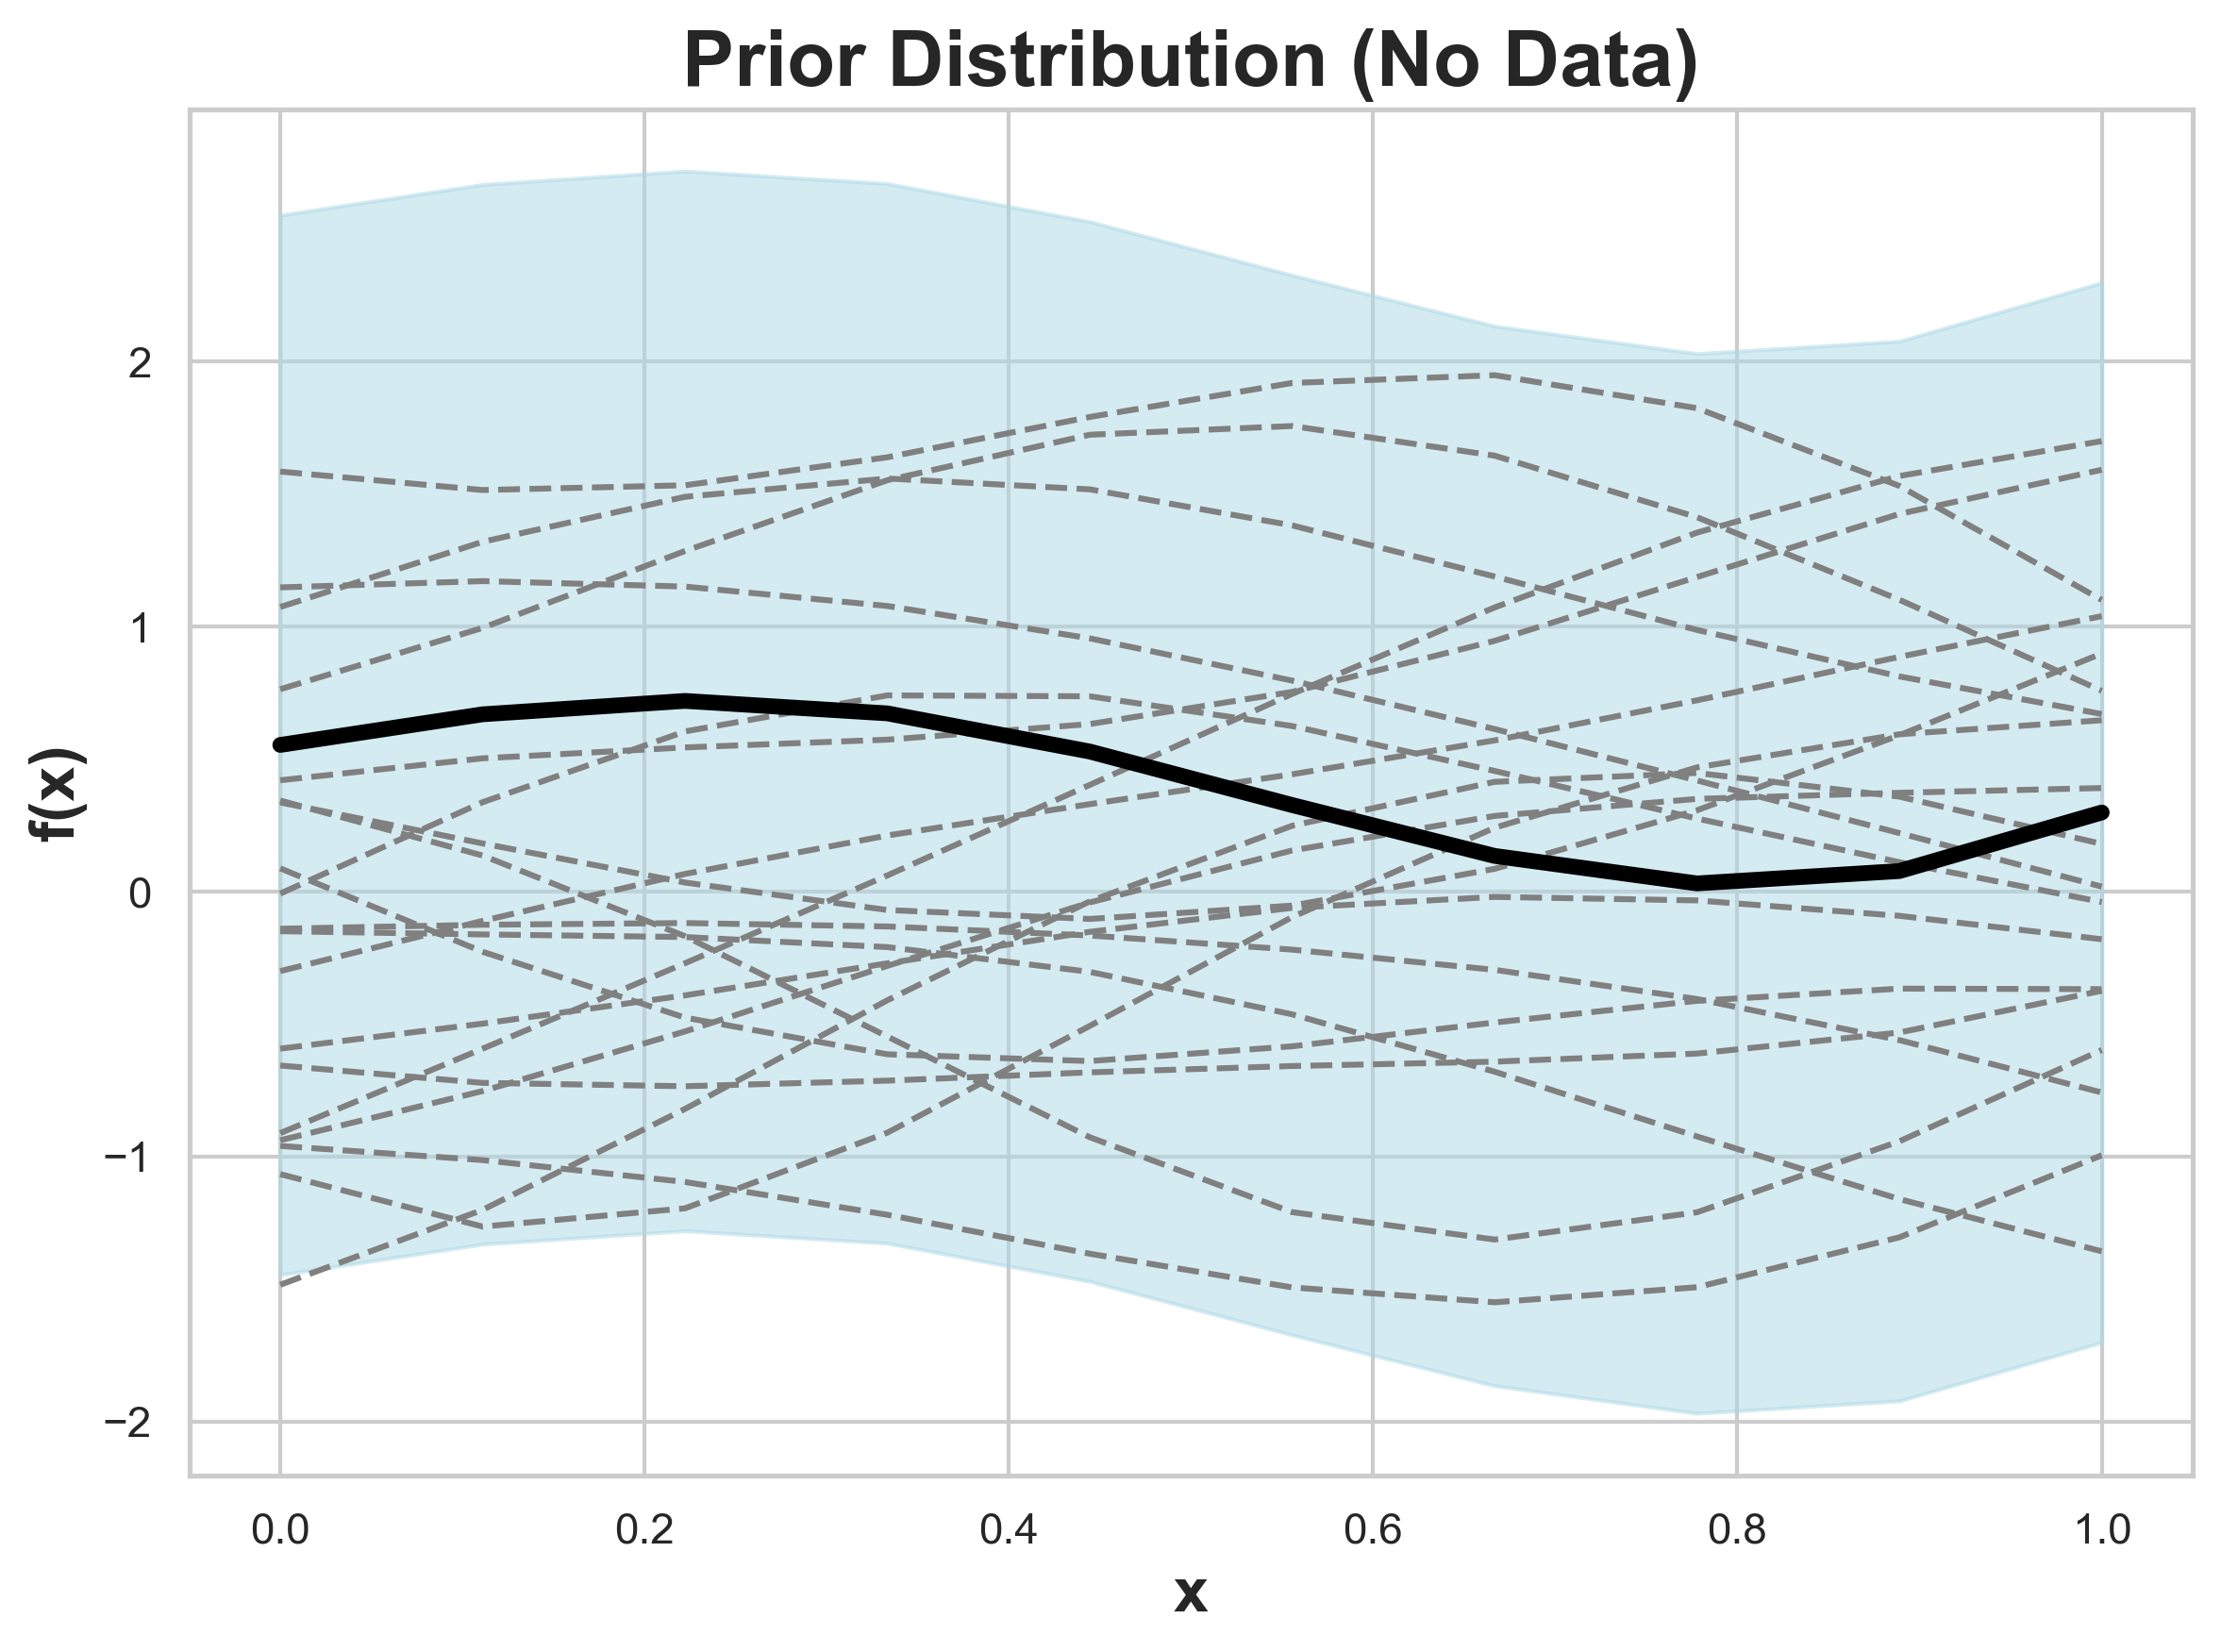
\includegraphics[width=\textwidth]{LatexPlots/1dplots/Prior_Distribution.png}
        \caption{Prior Distribution}
    \end{subfigure}
    \begin{subfigure}[b]{0.4\textwidth}
        \centering
        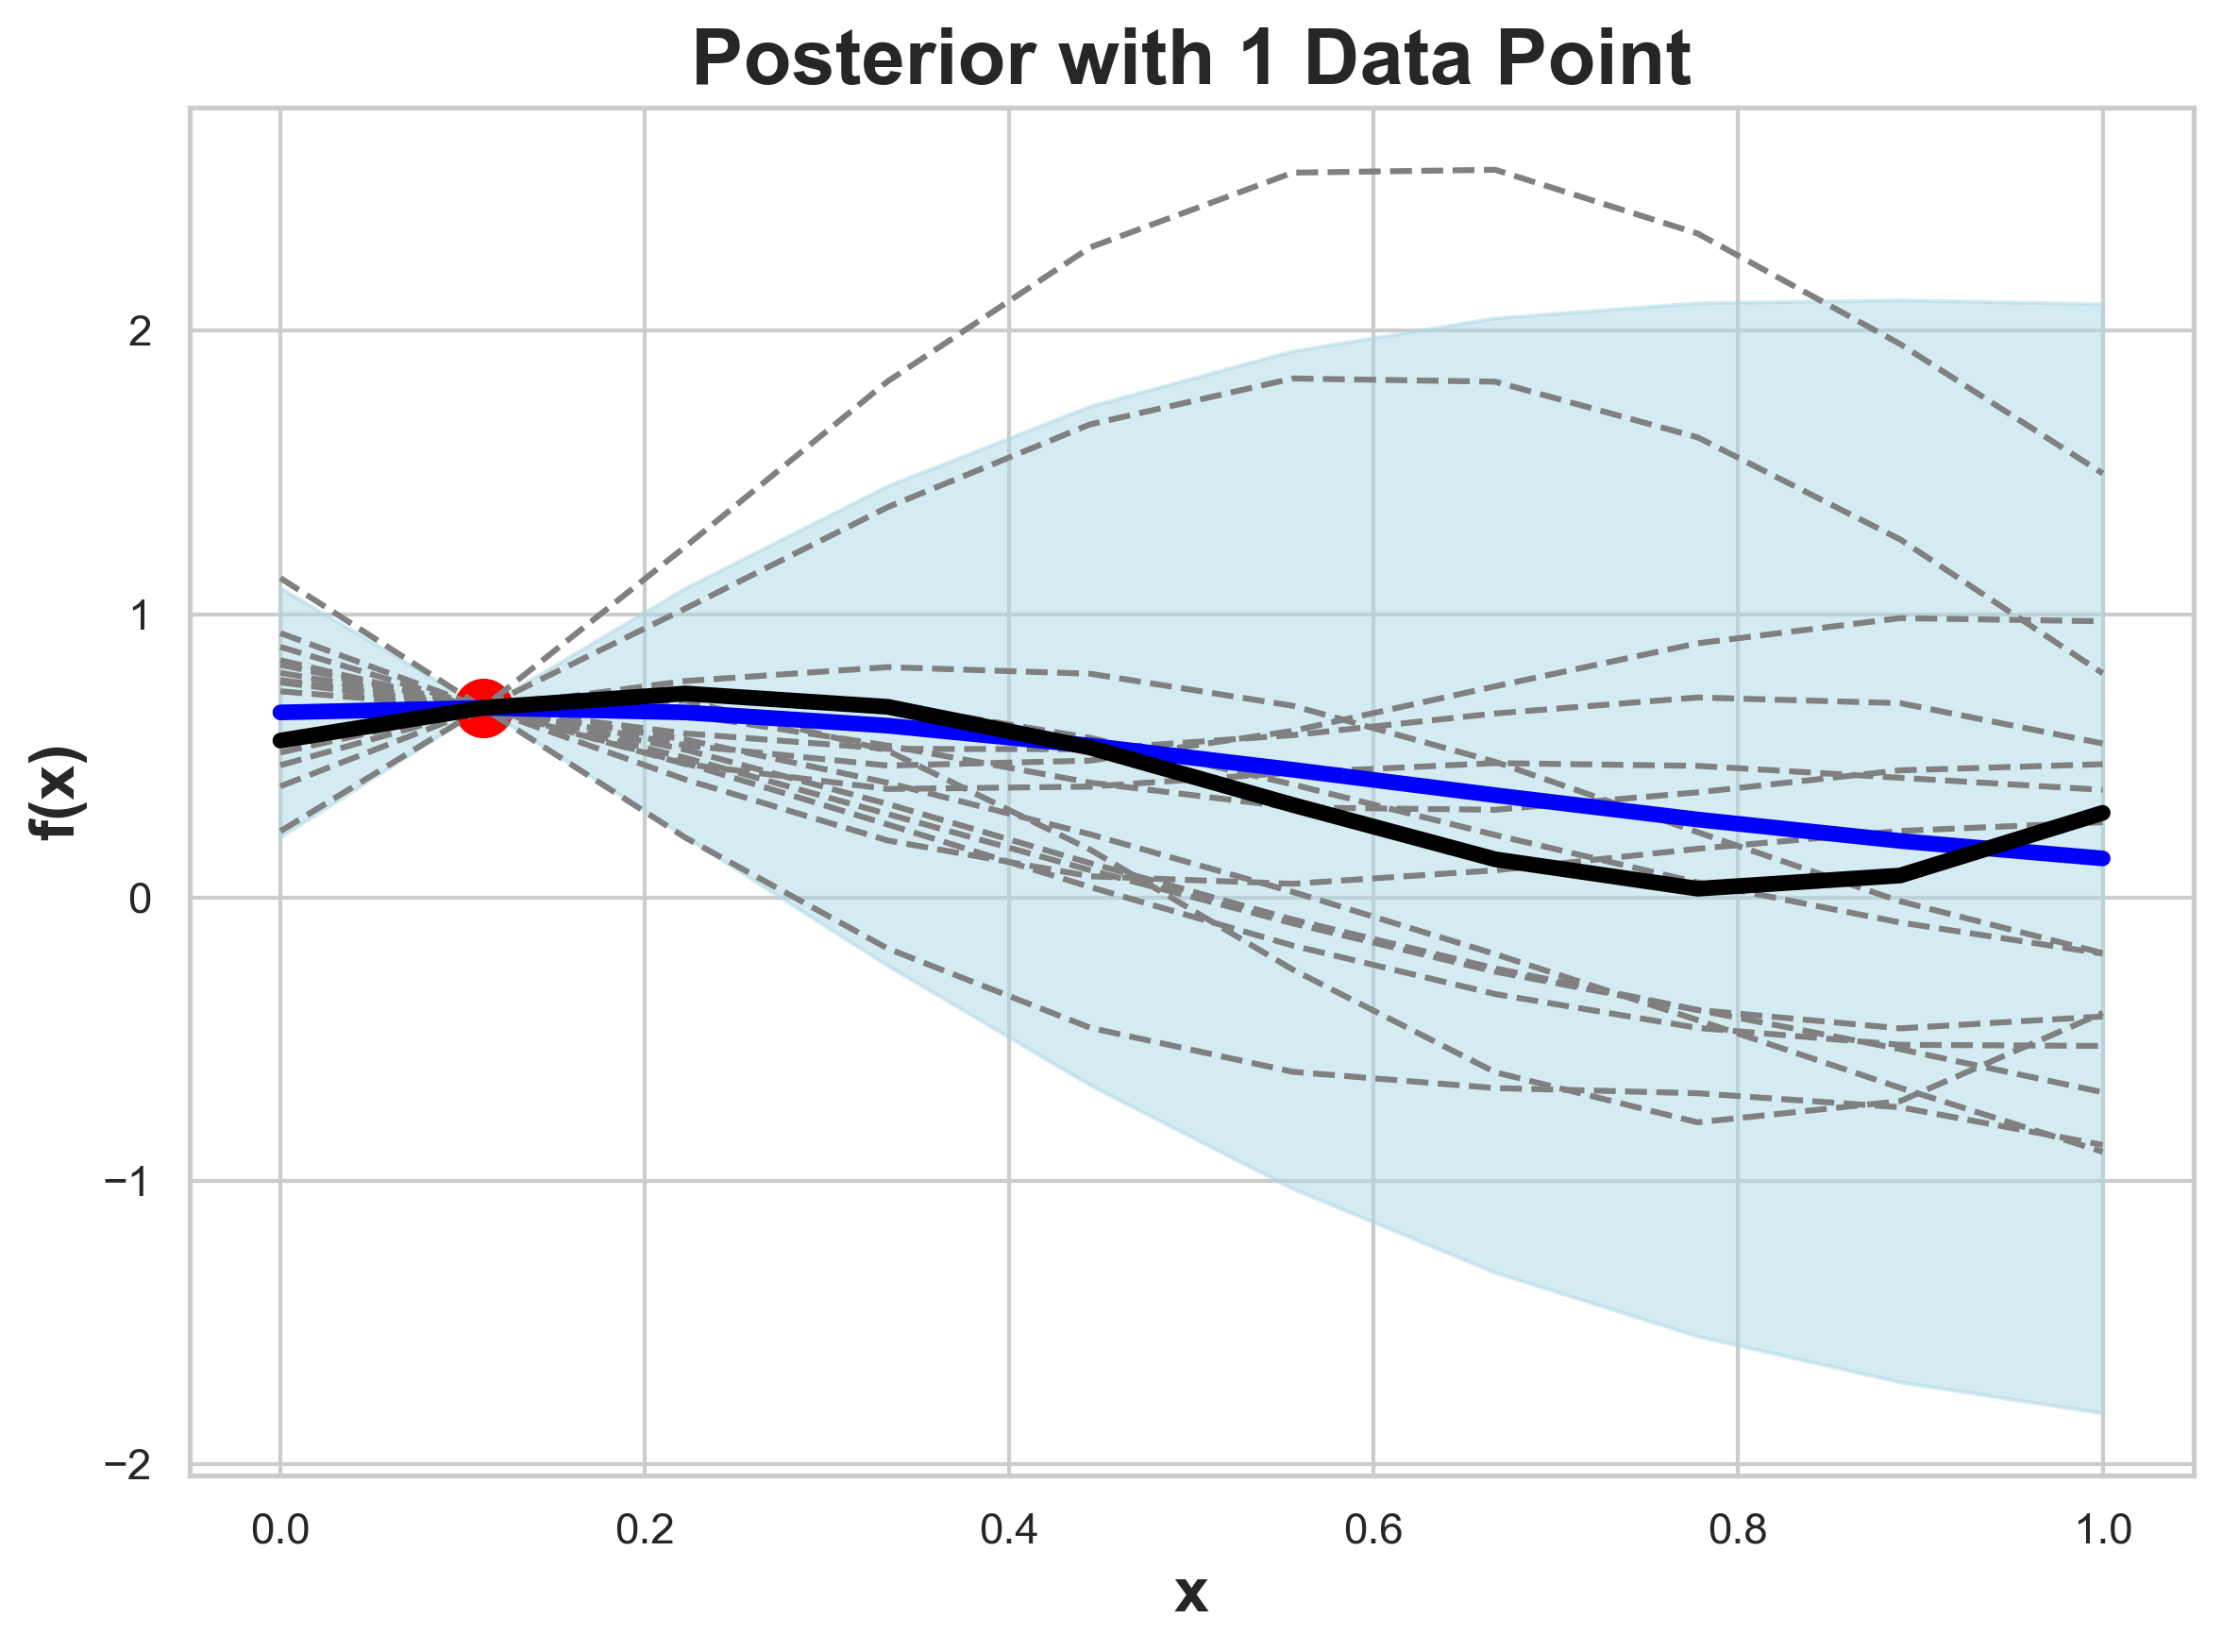
\includegraphics[width=\textwidth]{LatexPlots/1dplots/Posterior_1_Data_Point.png}
        \caption{Posterior: 1 Data Point}
    \end{subfigure}
    
    \vspace{0.5cm}
    
    \begin{subfigure}[b]{0.4\textwidth}
        \centering
        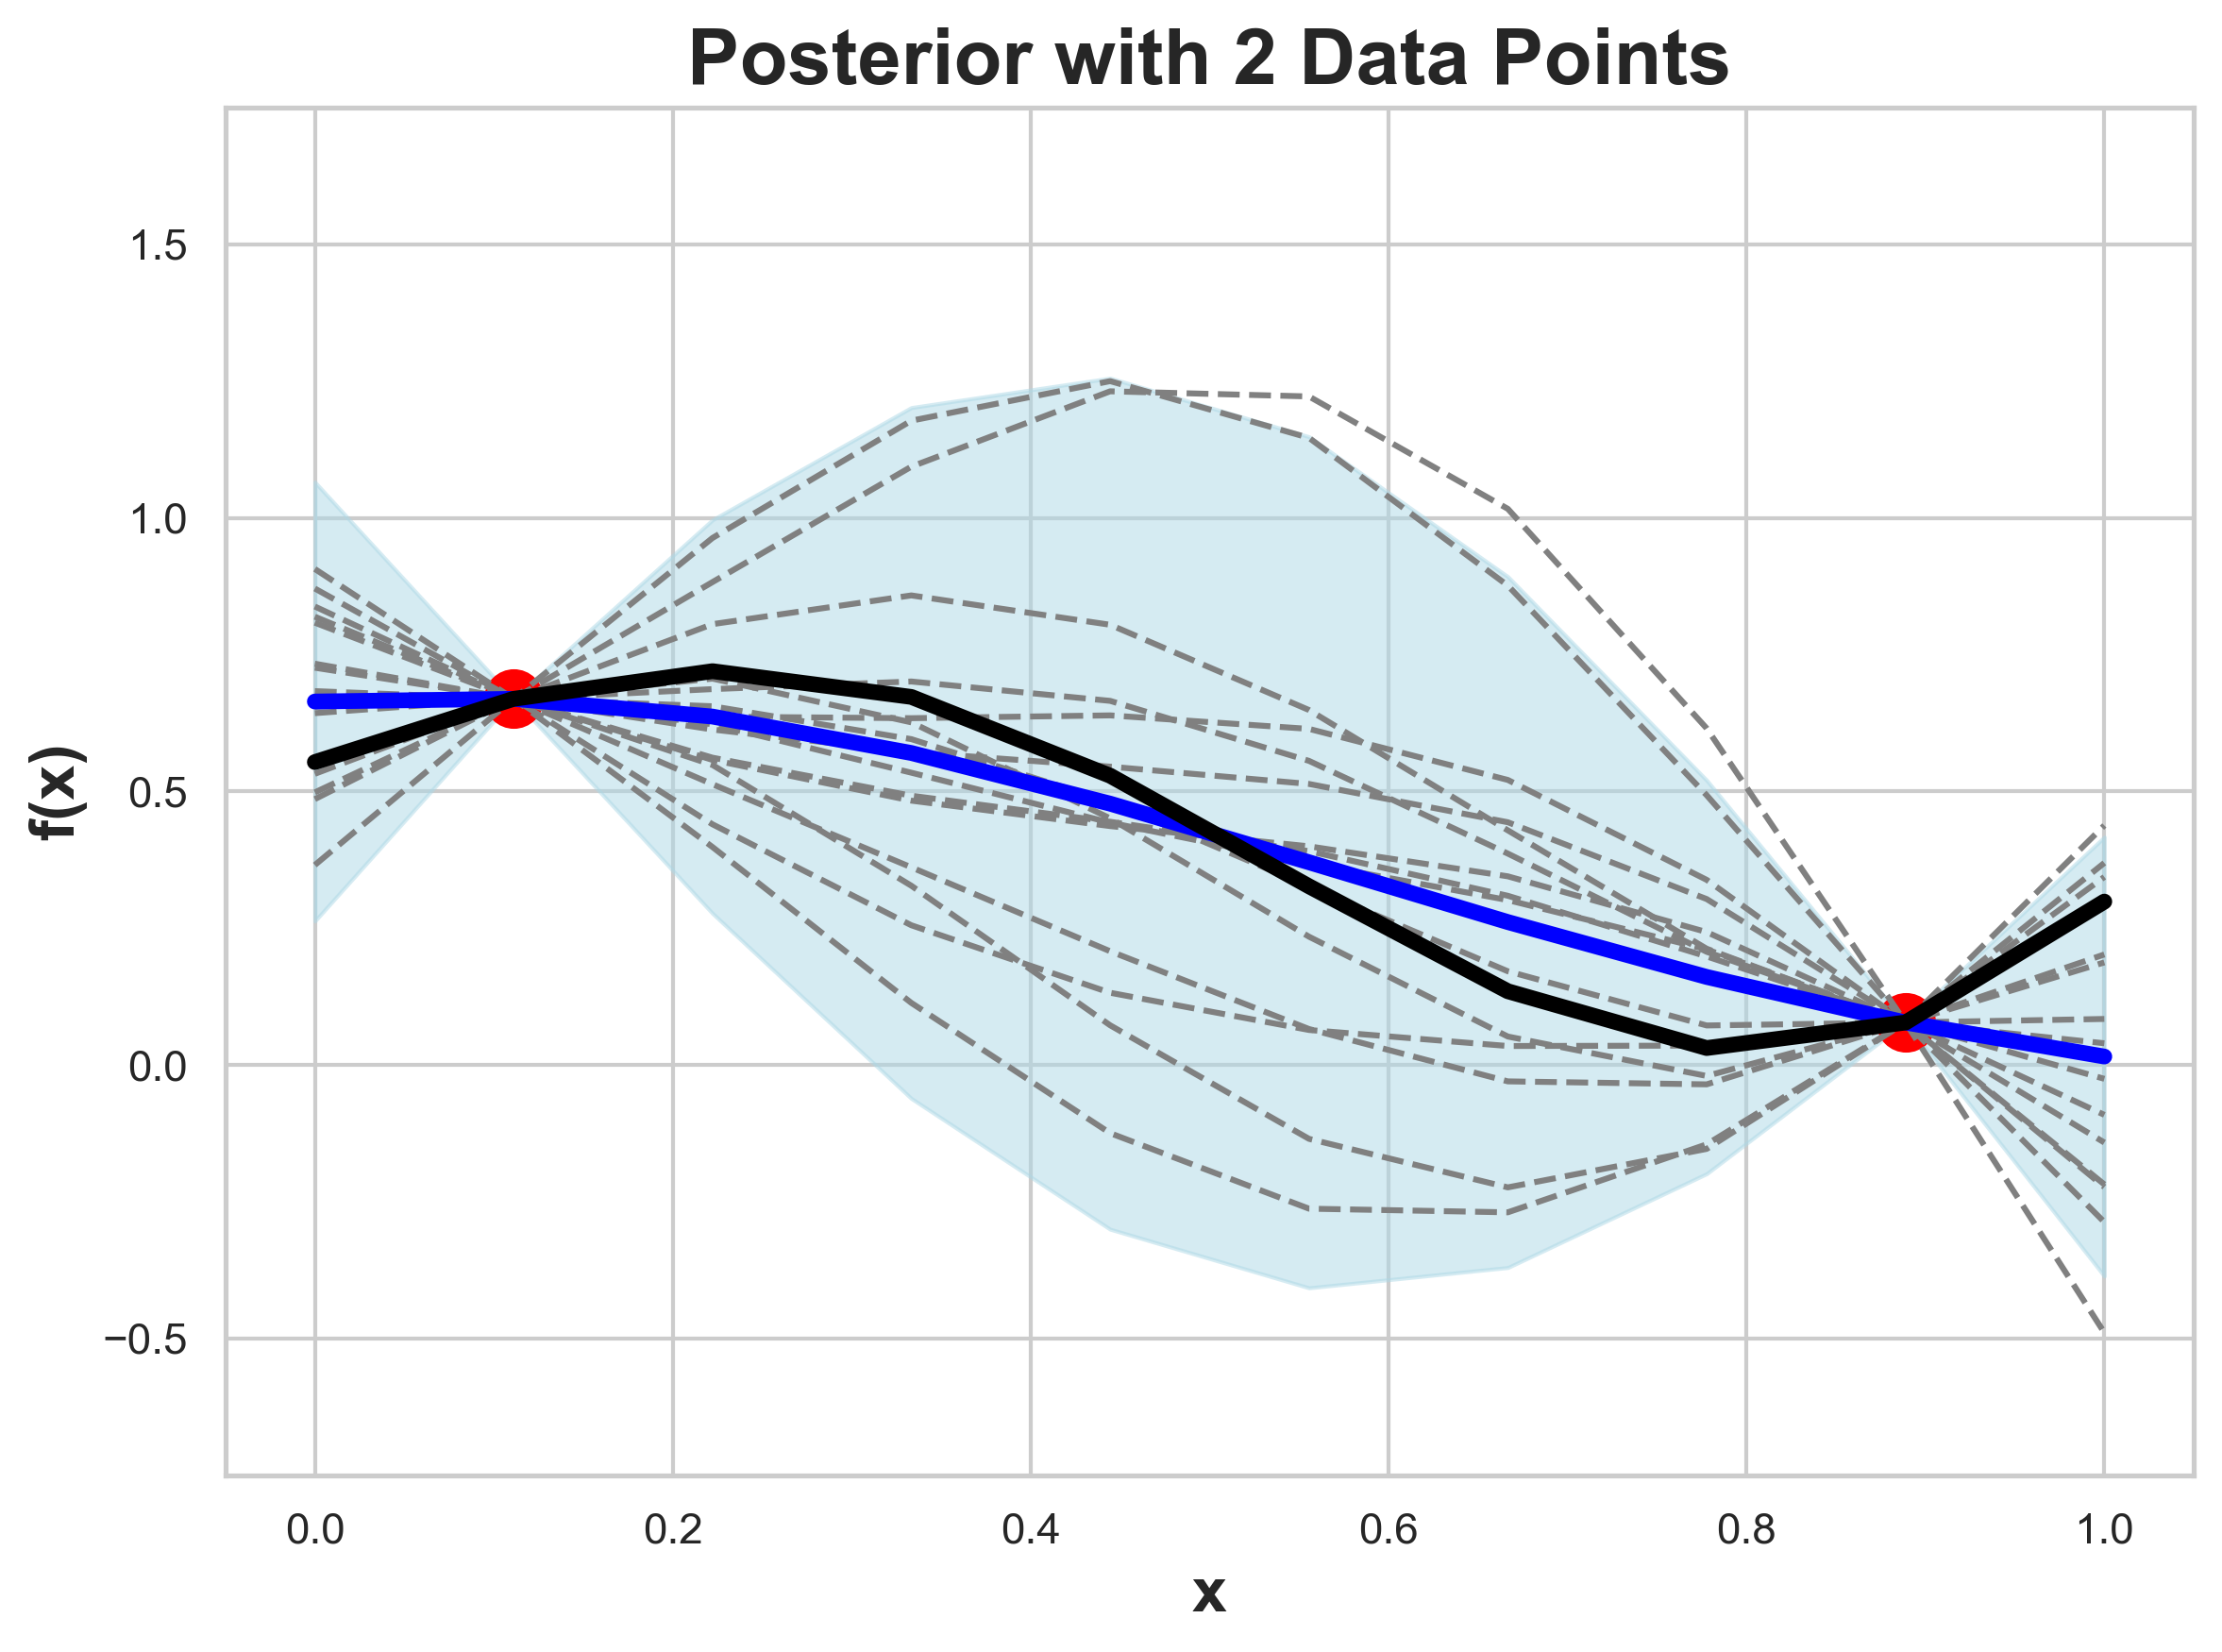
\includegraphics[width=\textwidth]{LatexPlots/1dplots/Posterior_2_Data_Points.png}
        \caption{Posterior: 2 Data Points}
    \end{subfigure}
    \begin{subfigure}[b]{0.4\textwidth}
        \centering
        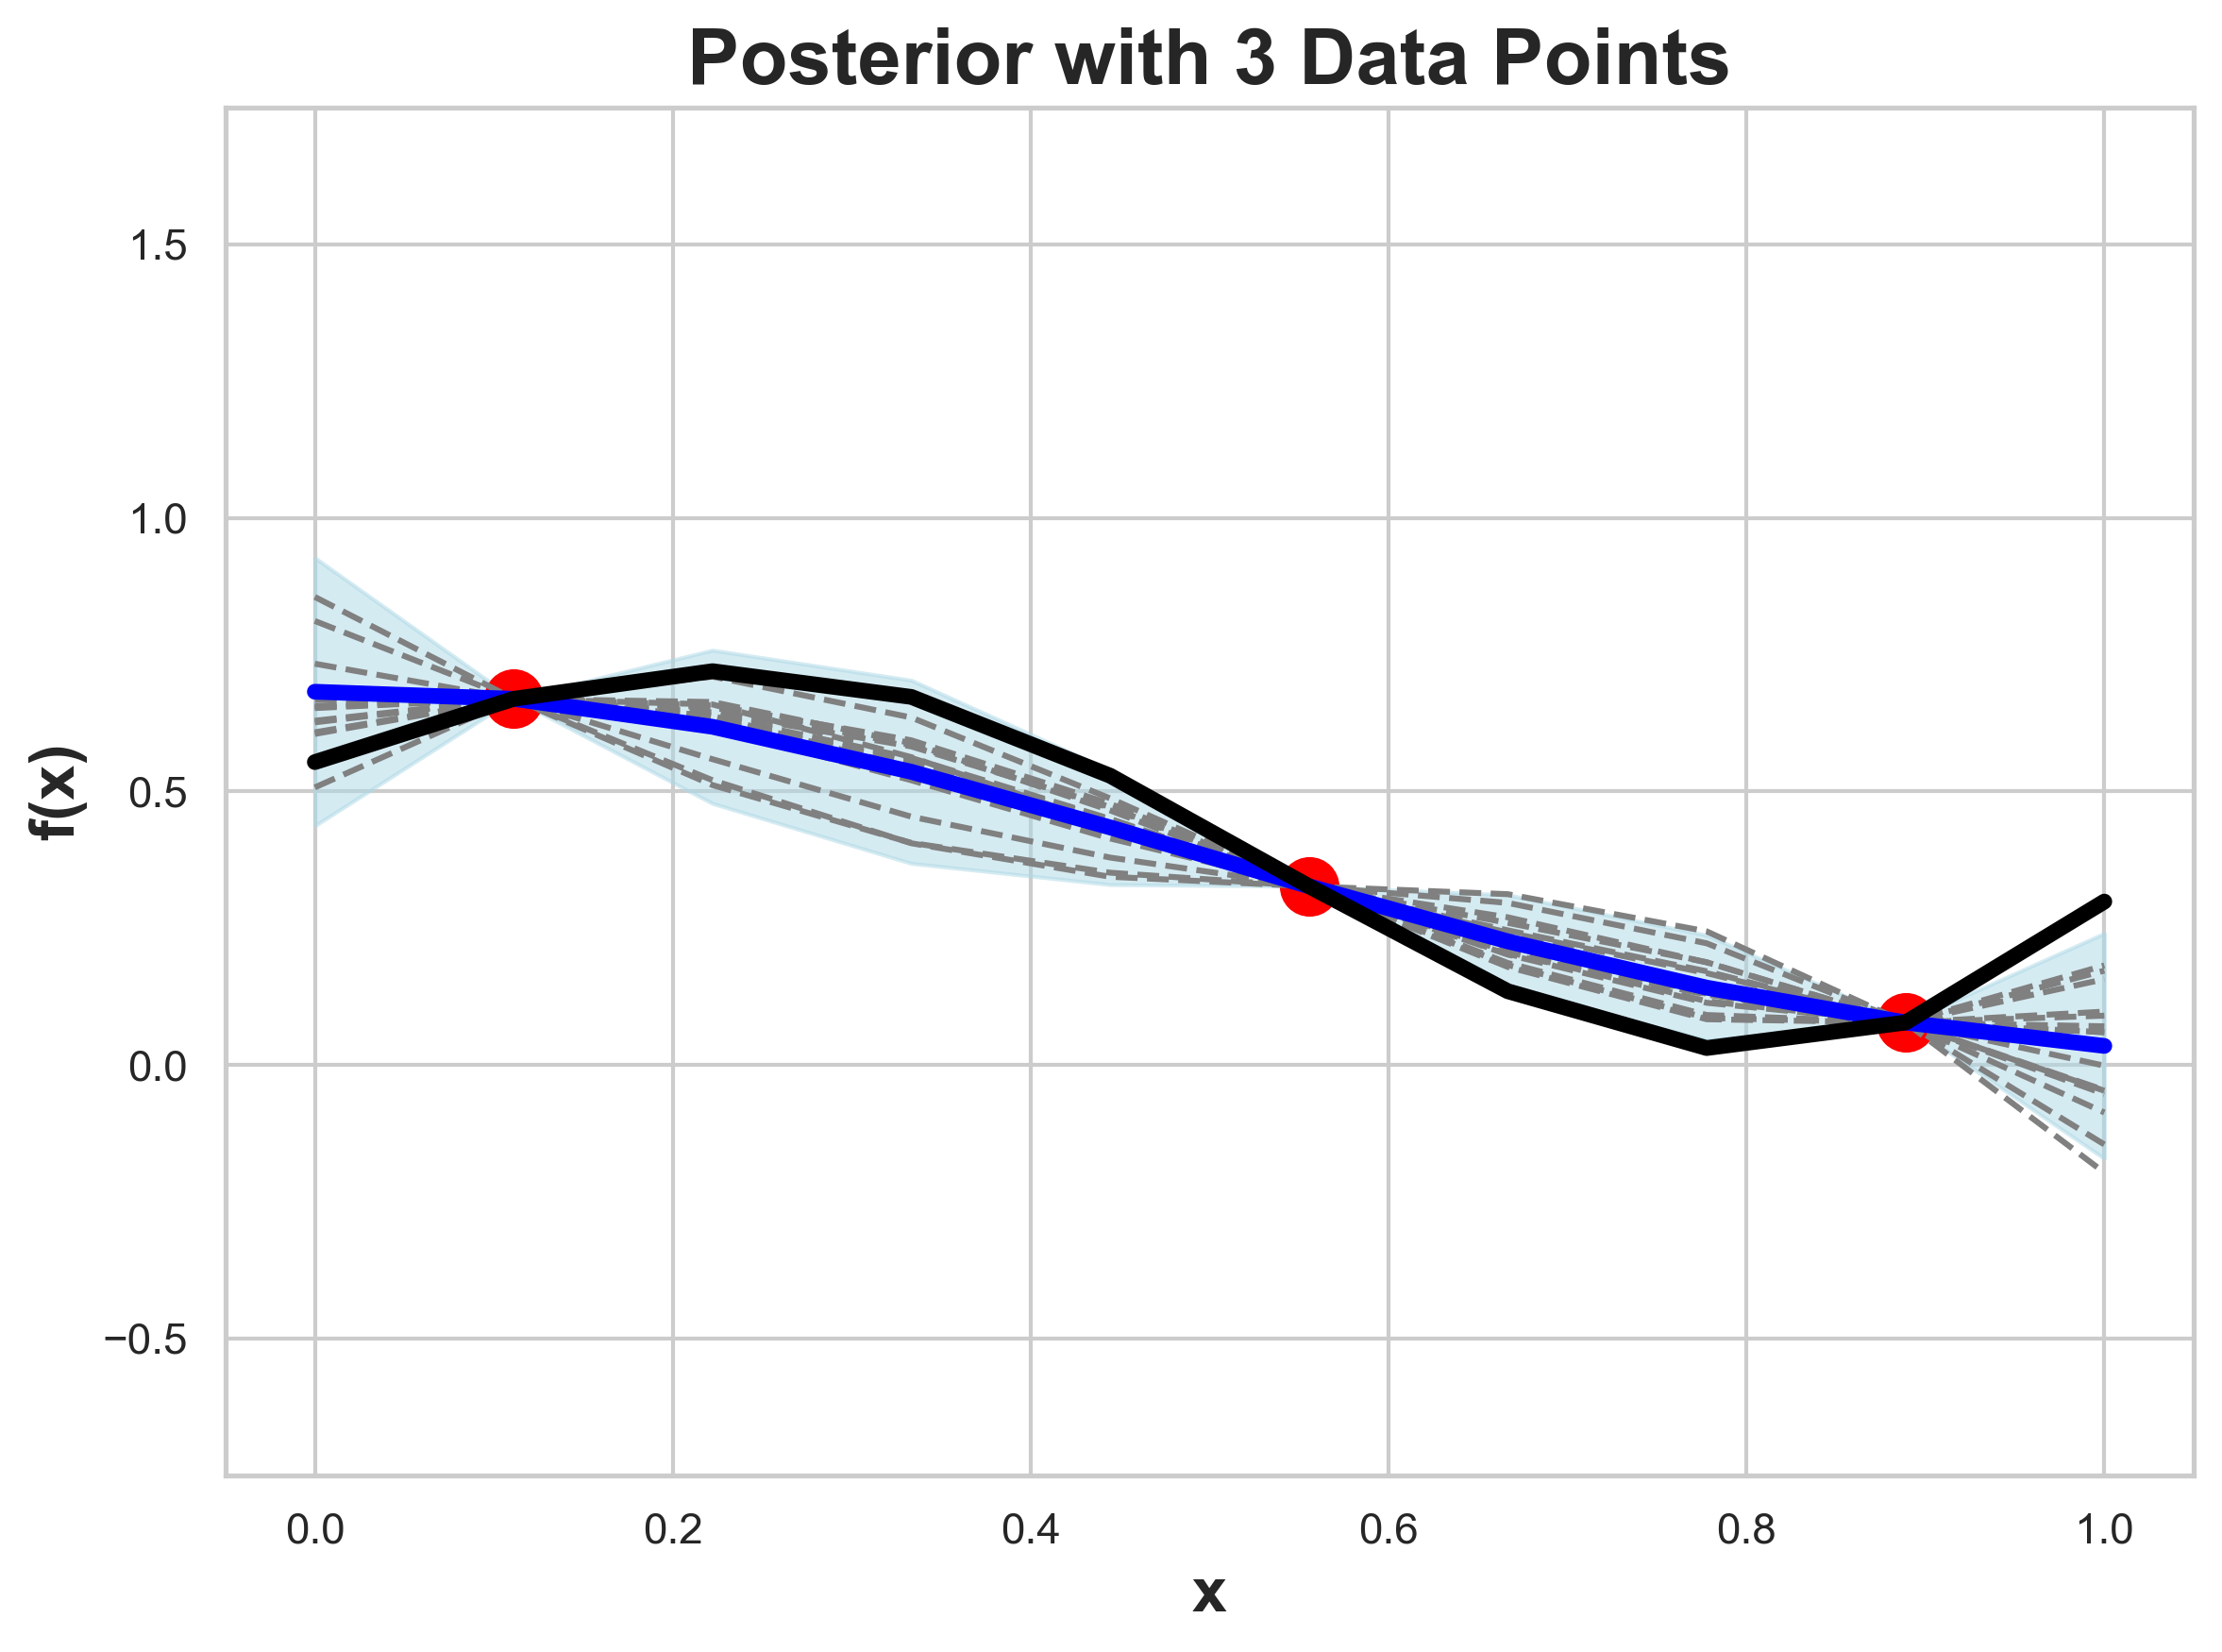
\includegraphics[width=\textwidth]{LatexPlots/1dplots/Posterior_3_Data_Points.png}
        \caption{Posterior: 3 Data Points}
    \end{subfigure}

    \caption{1D Gaussian Process Regression: Prior to Posterior. This sequence shows how the GP prior transforms into a posterior as more data points are added. The RBF kernel was used with hyper-parameters: $l = 1$, $\sigma^2 = 0.5$.}
\end{figure}


\subsection{Kernel Functions}
\label{sec: Kernels}
In Section~\ref{sec: priortoposterior}, we derived the mean and variance for the posterior distribution (Equations~\ref{eq: 2} and~\ref{eq: 3}). These quantities depend explicitly on the choice of kernel function, which encodes prior assumptions about the smoothness and structure of the functions we expect. In this section, we explore different types of kernels and discuss how they affect samples from the posterior distribution.

\noindent
As described in~\cite{rasmussen2006gaussian}, kernel functions can be broadly divided into two main categories: \textbf{stationary} and \textbf{non-stationary} kernels. Additional examples and insights into the construction and use of these kernels are provided in~\cite{duvenaud2014kernel}, which we also reference throughout this section.

\paragraph{Stationary Kernels:}  
A stationary kernel depends only on the relative distance between inputs, i.e., \( k(x, x') = k(|x - x'|) \). This means the statistical properties of the functions (such as smoothness, variance, and lengthscale) remain the same throughout the input space. They encode the assumption that the function behaves similarly everywhere.

\subsubsection*{Examples of Stationary Kernels}
\begin{itemize}
    \item \textbf{Radial Basis Function (RBF) Kernel:}
    \[
    k(x, x') = \sigma_f^2 \exp\left( -\frac{(x - x')^2}{2\ell^2} \right)
    \]
    This kernel assumes smooth and infinitely differentiable functions, modeling local variations.

    \item \textbf{Rational Quadratic Kernel:}
    \[
    k(x, x') = \sigma_f^2 \left( 1 + \frac{(x - x')^2}{2 \alpha \ell^2} \right)^{-\alpha}
    \]
    This kernel can be seen as a scale mixture of RBF kernels, allowing for multi-scale behavior.

    \item \textbf{Periodic Kernel:}
    \[
    k(x, x') = \sigma_f^2 \exp\left( -\frac{2}{\ell^2} \sin^2\left( \frac{\pi (x - x')}{p} \right) \right)
    \]
    This kernel models repeating structures with period \( p \).

    \item \textbf{Matern Kernel (general form):}
    \[
    k(x, x') = \sigma_f^2 \frac{2^{1-\nu}}{\Gamma(\nu)} \left( \frac{\sqrt{2\nu} |x - x'|}{\ell} \right)^\nu K_\nu\left( \frac{\sqrt{2\nu} |x - x'|}{\ell} \right)
    \]
    The Matern kernel allows for controlling the smoothness of functions via the parameter \( \nu \).

    \item \textbf{Laplace (Exponential) Kernel:}
    \[
    k(x, x') = \sigma_f^2 \exp\left( -\gamma |x - x'| \right)
    \]
    Equivalent to the Matern kernel with \( \nu = \frac{1}{2} \), this kernel models rougher functions.
\end{itemize}

\paragraph{Non-Stationary Kernels:}  
In contrast, non-stationary kernels depend on the absolute location of the inputs, i.e., \( k(x, x') \) cannot be written purely as a function of \( |x - x'| \). This allows the modeled function's properties (e.g., smoothness or variance) to vary across the input space.

\subsubsection*{Example of a Non-Stationary Kernel}
\begin{itemize}
    \item \textbf{Linear (Dot Product) Kernel:}
    \[
    k(x, x') = \sigma_b^2 + x^\top x'
    \]
    This kernel grows with the similarity (inner product) between inputs, and it allows the function to vary globally. Since it depends directly on the values of \( x \) and \( x' \), not just their difference, it is non-stationary. It is particularly useful for modeling linear trends.
\end{itemize}


\subsubsection*{Visual Comparison of Kernels}

To further illustrate the effects of different kernel functions, Table~\ref{tab:kernel-examples} provides visual comparisons of each kernel's structure, as well as samples drawn from their corresponding Gaussian process priors. These examples highlight how the choice of kernel influences the shape, smoothness, and general behavior of functions drawn from a GP. Each kernel is plotted with standard hyperparameter settings to allow for consistent comparison across types.


\begin{table}[H]
    \centering
    \renewcommand{\arraystretch}{4} % Slightly tighter rows
    \setlength{\tabcolsep}{2pt} % Tighter columns
    \small % Smaller text to fit content

    \begin{tabular}{|>{\centering\arraybackslash}m{2cm}|*{6}{>{\centering\arraybackslash}m{2.3cm}|}} 
        \hline
        \textbf{Kernel name:} & \textbf{RBF (SE)} & \textbf{Rational Quadratic} & \textbf{Periodic} & \textbf{Matern} & \textbf{Laplace} & \textbf{Linear (Dot Product)} \\ 
        \hline
        \textbf{Plot of $k(x, x')$:} & 
        \adjustbox{valign=c}{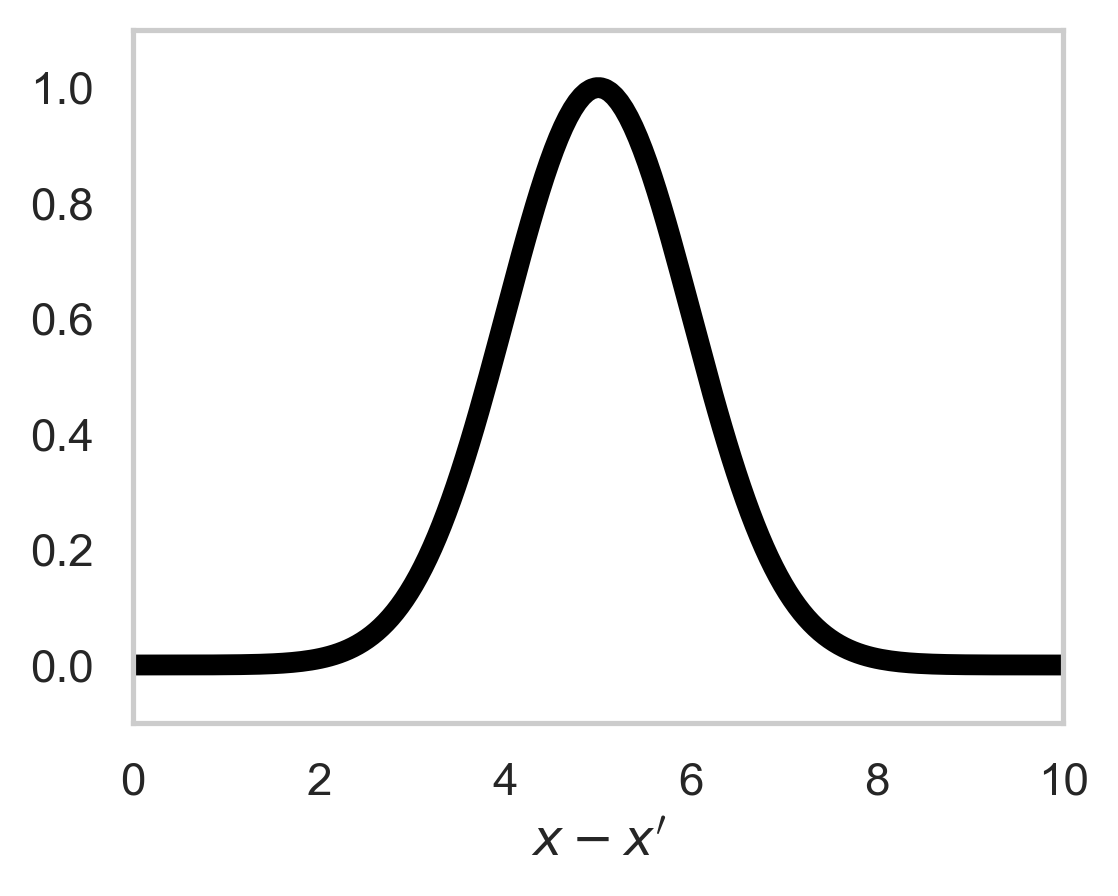
\includegraphics[width=2.25cm]{LatexPlots/1dplots/Kernel_RBF_SE.png}} & 
        \adjustbox{valign=c}{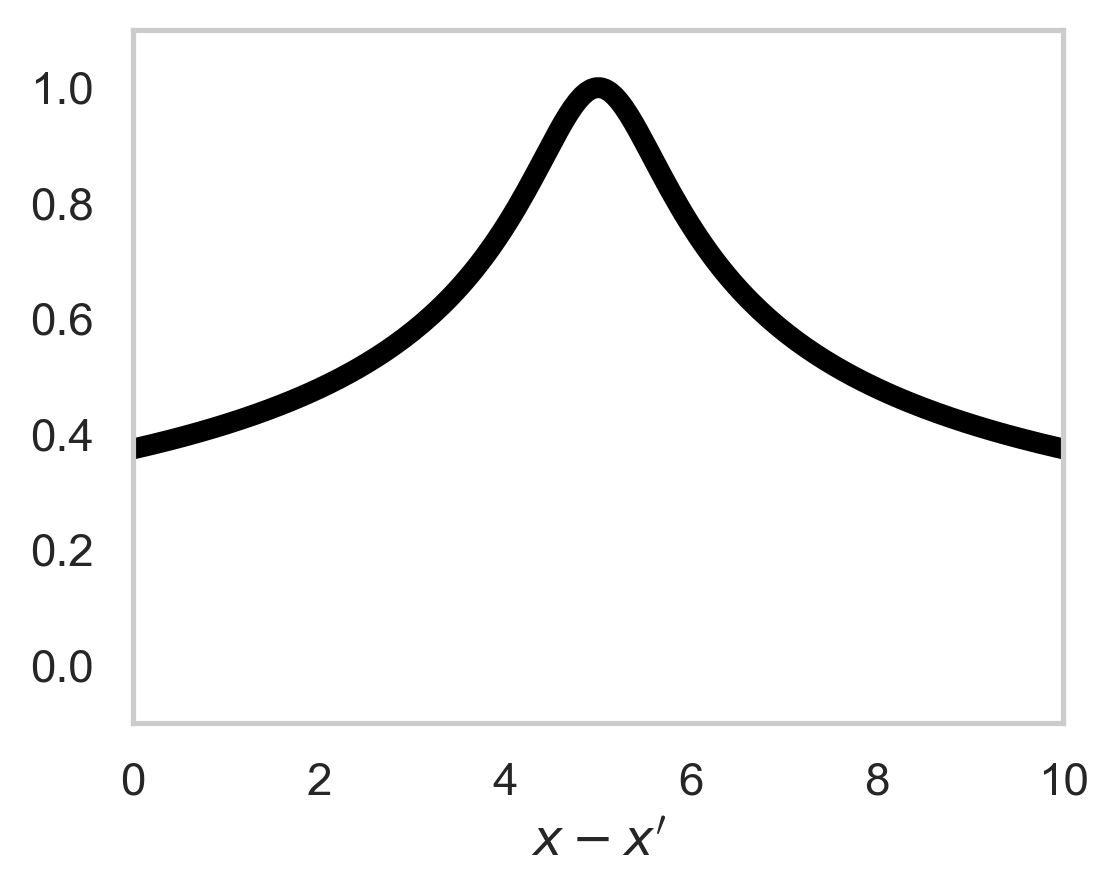
\includegraphics[width=2.25cm]{LatexPlots/1dplots/Kernel_Rational_Quadratic.png}} & 
        \adjustbox{valign=c}{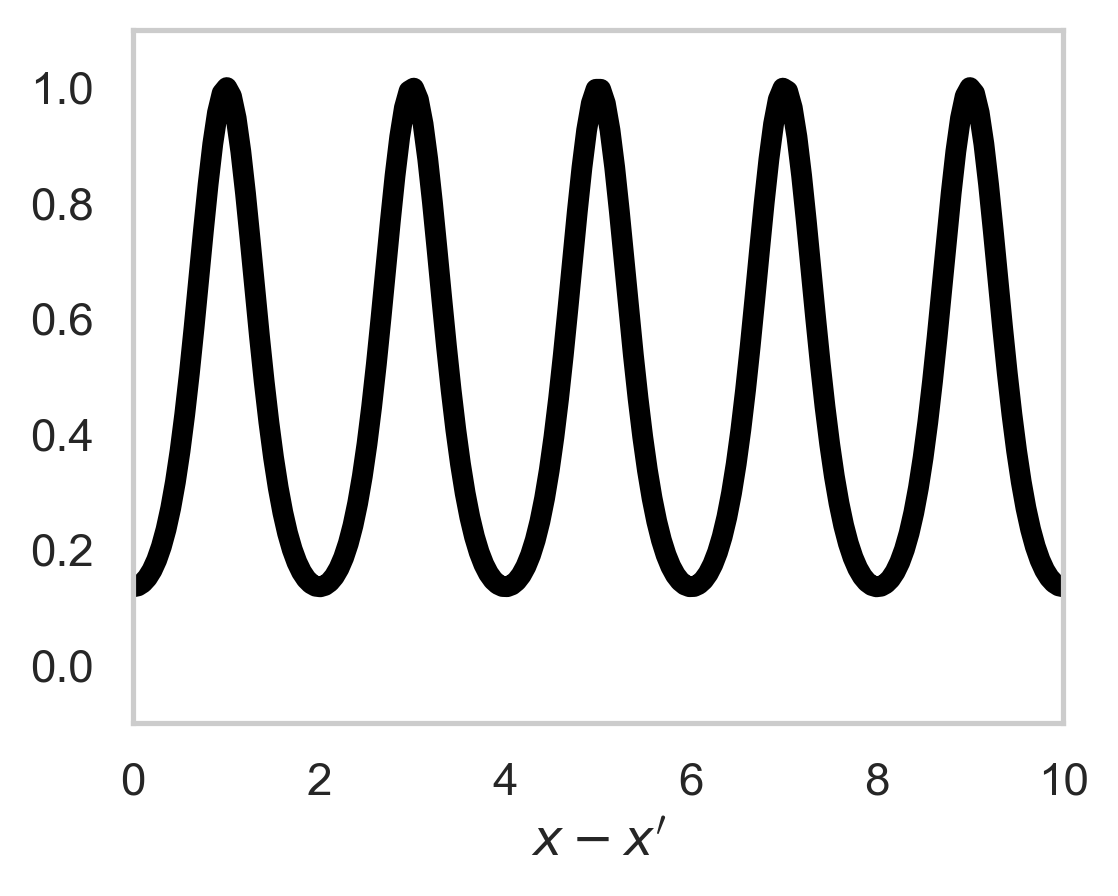
\includegraphics[width=2.25cm]{LatexPlots/1dplots/Kernel_Periodic.png}} & 
        \adjustbox{valign=c}{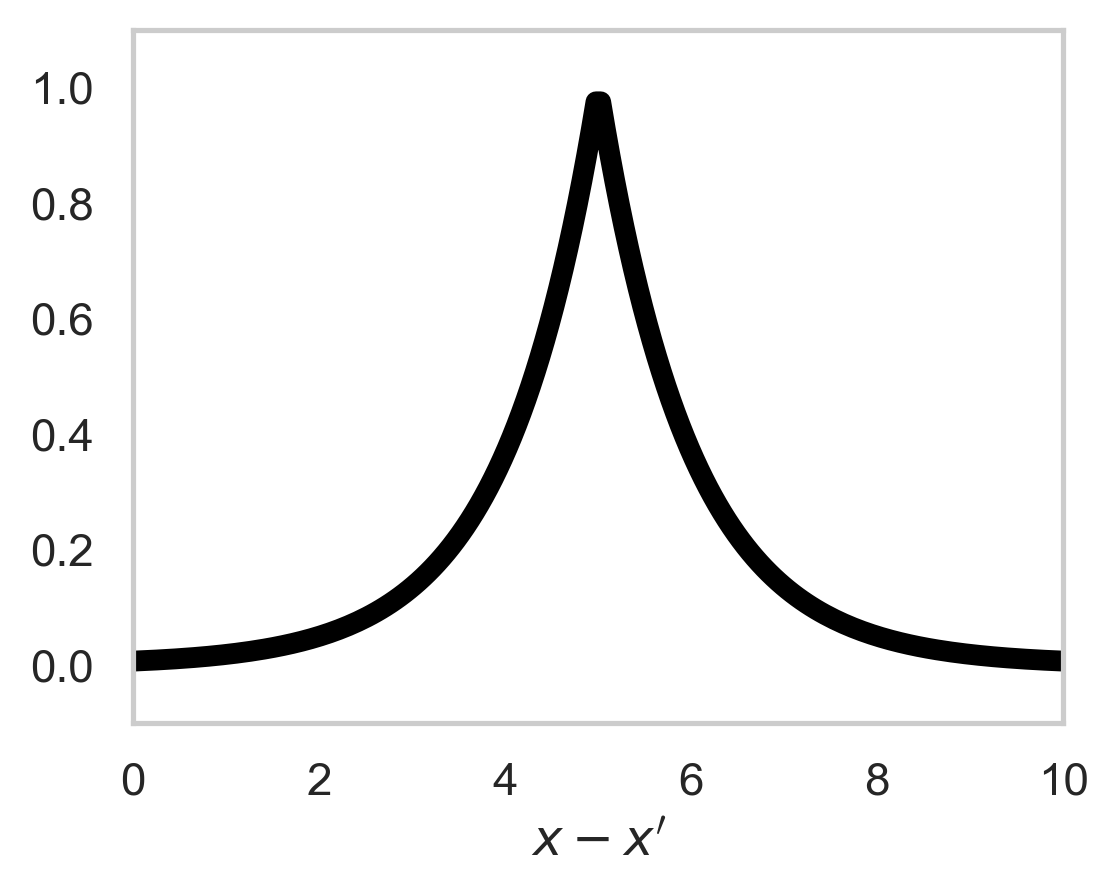
\includegraphics[width=2.25cm]{LatexPlots/1dplots/Kernel_Matern_nu05.png}} & 
        \adjustbox{valign=c}{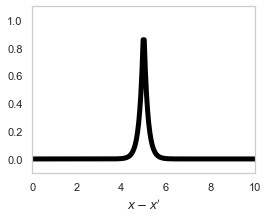
\includegraphics[width=2.25cm]{LatexPlots/1dplots/Kernel_Laplace_Exponential.png}} & 
        \adjustbox{valign=c}{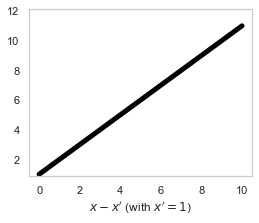
\includegraphics[width=2.25cm]{LatexPlots/1dplots/Kernel_Linear_Dot_Product.png}} \\ 
        \hline
        \textbf{GP Prior Samples:} & 
        \adjustbox{valign=c}{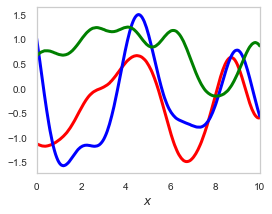
\includegraphics[width=2.25cm]{LatexPlots/1dplots/KernelSample_RBF_SE.png}} & 
        \adjustbox{valign=c}{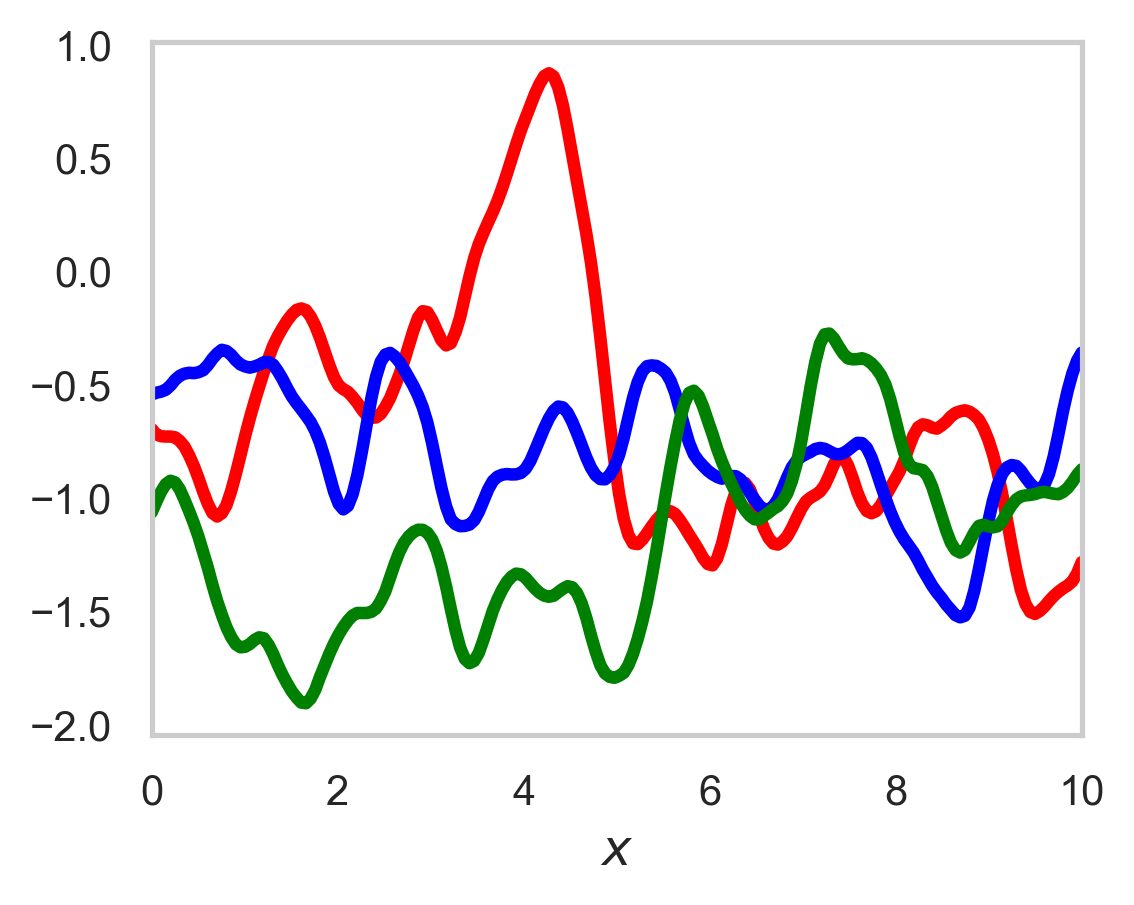
\includegraphics[width=2.25cm]{LatexPlots/1dplots/KernelSample_Rational_Quadratic.png}} & 
        \adjustbox{valign=c}{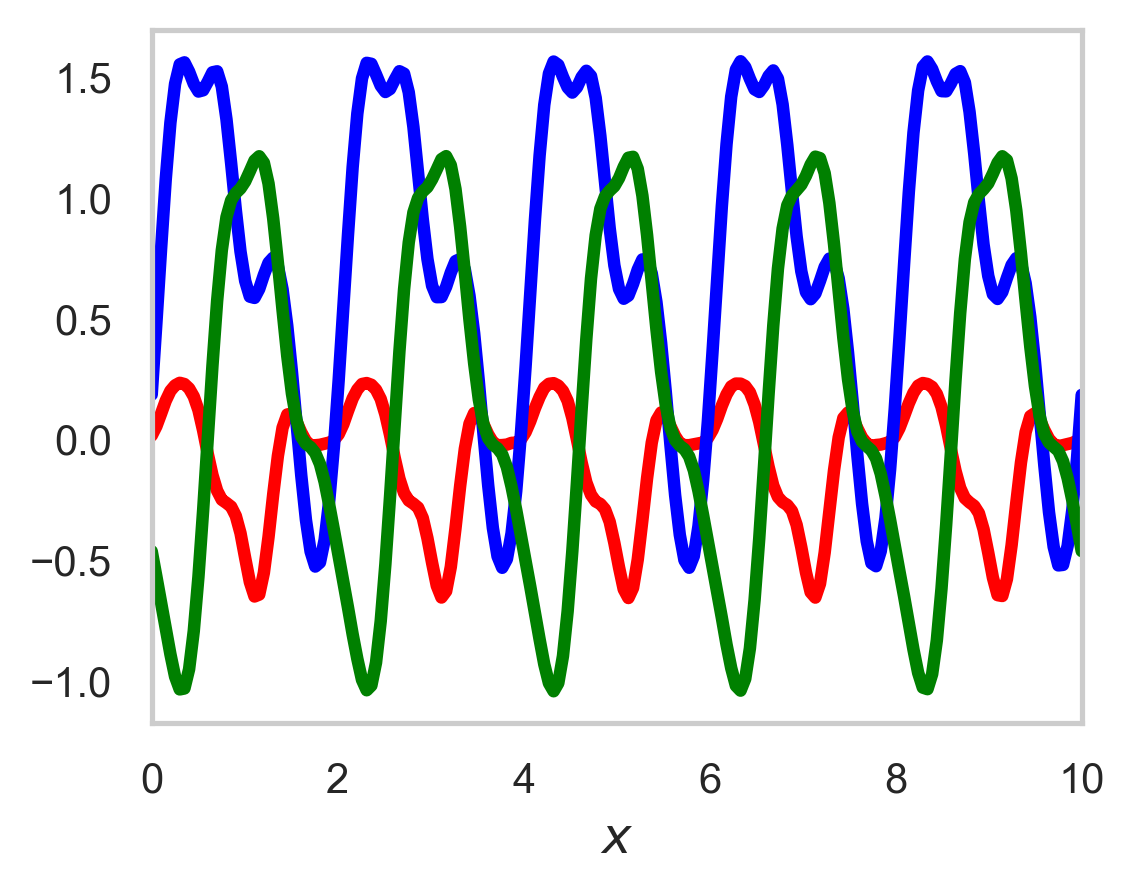
\includegraphics[width=2.25cm]{LatexPlots/1dplots/KernelSample_Periodic.png}} & 
        \adjustbox{valign=c}{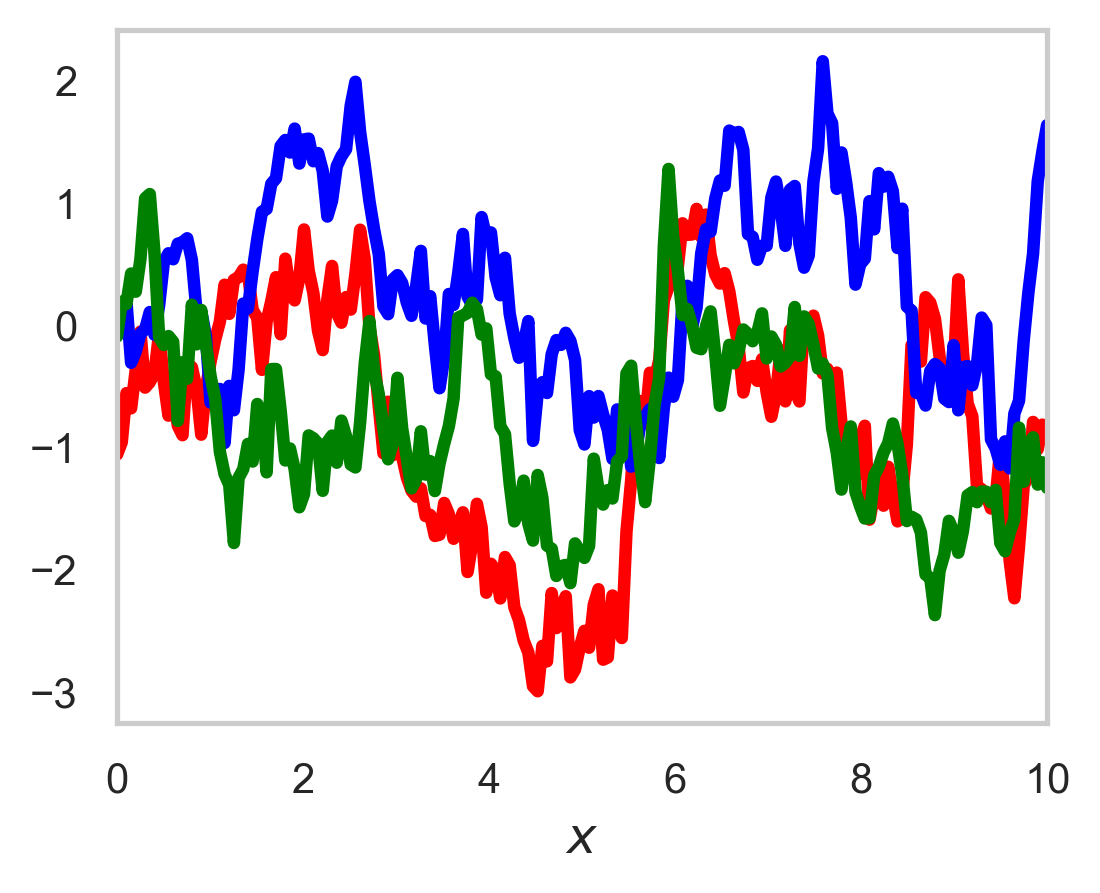
\includegraphics[width=2.25cm]{LatexPlots/1dplots/KernelSample_Matern_nu05.png}} & 
        \adjustbox{valign=c}{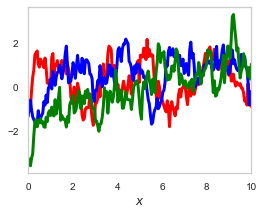
\includegraphics[width=2.25cm]{LatexPlots/1dplots/KernelSample_Laplace_Exponential.png}} & 
        \adjustbox{valign=c}{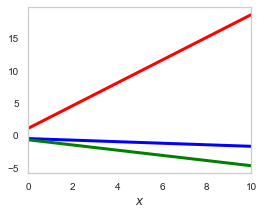
\includegraphics[width=2.25cm]{LatexPlots/1dplots/KernelSample_Linear_Dot_Product.png}} \\ 
        \hline
        \textbf{Structure type:} & 
        Local variation & 
        Multi-scale local variation & 
        Repeating structure & 
        Rough to smooth & 
        Rougher variation & 
        Linear functions \\ 
        \hline
    \end{tabular}
    \caption{
        Visual comparison of common kernel functions and their effect on Gaussian process priors. 
        Each column shows the kernel shape $k(x, x')$, samples from the corresponding GP prior, and a summary of the structure it imposes. 
        All kernels were evaluated using a lengthscale parameter $\ell = 1$ (except where noted). 
        For the Matern kernel, $\nu = 0.5$; Laplace kernel, $\gamma = 6$; Rational Quadratic kernel, $\alpha = 0.25$; and Periodic kernel, period $p = 2$.
        }
    \label{tab:kernel-examples}
\end{table}


\subsection{Handling Noise in our Data}
\label{sec: Handlingnoise}

So far, our discussion has assumed noise-free observations. However, real-world data is rarely clean—measurements often include some form of uncertainty. To make our Gaussian Process models more realistic and applicable, we now explore how to incorporate noise into the GP framework.

\bigskip

\noindent
We model noise by assuming that the observations $y$ are related to the latent function values $f$ through additive Gaussian noise:
\[
y = f + \epsilon, \quad \epsilon \sim \mathcal{N}(0, \sigma_n^2 I),
\]
where $\sigma_n^2$ is the noise variance. We now have:
\[
f \sim \mathcal{N}(0, K)
\]
and 
\begin{equation}\label{eq: 4}
y \sim \mathcal{N}(0, K+\sigma_n^2 I)
\end{equation}

\bigskip

which leads to a revised posterior:
\[
m(f_*) = K_*^T (K + \sigma_n^2 I)^{-1} y,
\]
\[
\text{Var}(f_*) = K_{**} - K_*^T (K + \sigma_n^2 I)^{-1} K_*.
\]

\bigskip

\noindent
There are three common approaches to handling noise in GPR:

\begin{itemize}
    \item \textbf{Noise as a Hyper-parameter (Homoscedastic Noise)}:  
    Here, we assume that all observations have the same level of noise, i.e., the noise is constant throughout the dataset:
    \[
    \sigma_i^2 = \sigma_n^2 \quad \forall i.
    \]
    This leads to a covariance matrix modified by adding a constant term to the diagonal:
    \[
    K(X, X) + \sigma_n^2 I = 
    \begin{bmatrix}
    k(x_1, x_1) + \sigma_n^2 & \cdots & k(x_1, x_n) \\
    \vdots & \ddots & \vdots \\
    k(x_n, x_1) & \cdots & k(x_n, x_n) + \sigma_n^2
    \end{bmatrix}.
    \]
    The noise variance $\sigma_n^2$ is treated as a learnable hyper-parameter during model training.

    \item \textbf{Known Noise (Heteroscedastic Noise)}:  
    In this case, the noise variance changes across the input space—some observations are noisier than others. If we know the individual noise variances $\sigma_i^2$ for each training input $x_i$, we incorporate them by adding a diagonal noise matrix to the kernel:
    \[
    K(X, X) + \Sigma = 
    \begin{bmatrix}
    k(x_1, x_1) + \sigma_1^2 & \cdots & k(x_1, x_n) \\
    \vdots & \ddots & \vdots \\
    k(x_n, x_1) & \cdots & k(x_n, x_n) + \sigma_n^2
    \end{bmatrix},
    \]
    where $\Sigma = \text{diag}(\sigma_1^2, \sigma_2^2, \dots, \sigma_n^2)$.

    \item \textbf{Monte Carlo Sampling of Noise}:  
    This technique can be used with either homoscedastic or heteroscedastic noise. Instead of modifying the kernel matrix directly, we explicitly simulate noise. We assume:
    \[
    \epsilon_i \sim \mathcal{N}(0, \sigma_i^2),
    \]
    and create new noisy training sets by adding a sampled noise value to each function value:
    \[
    y_i^{(s)} = f_i + \epsilon_i^{(s)}.
    \]
    Repeating this sampling multiple times allows us to generate multiple noisy versions of the dataset. We then average predictions over these Monte Carlo samples to better capture the uncertainty introduced by noise.
\end{itemize}

\begin{figure}[H]
    \centering
    \begin{subfigure}[b]{0.3\textwidth}
        \centering
        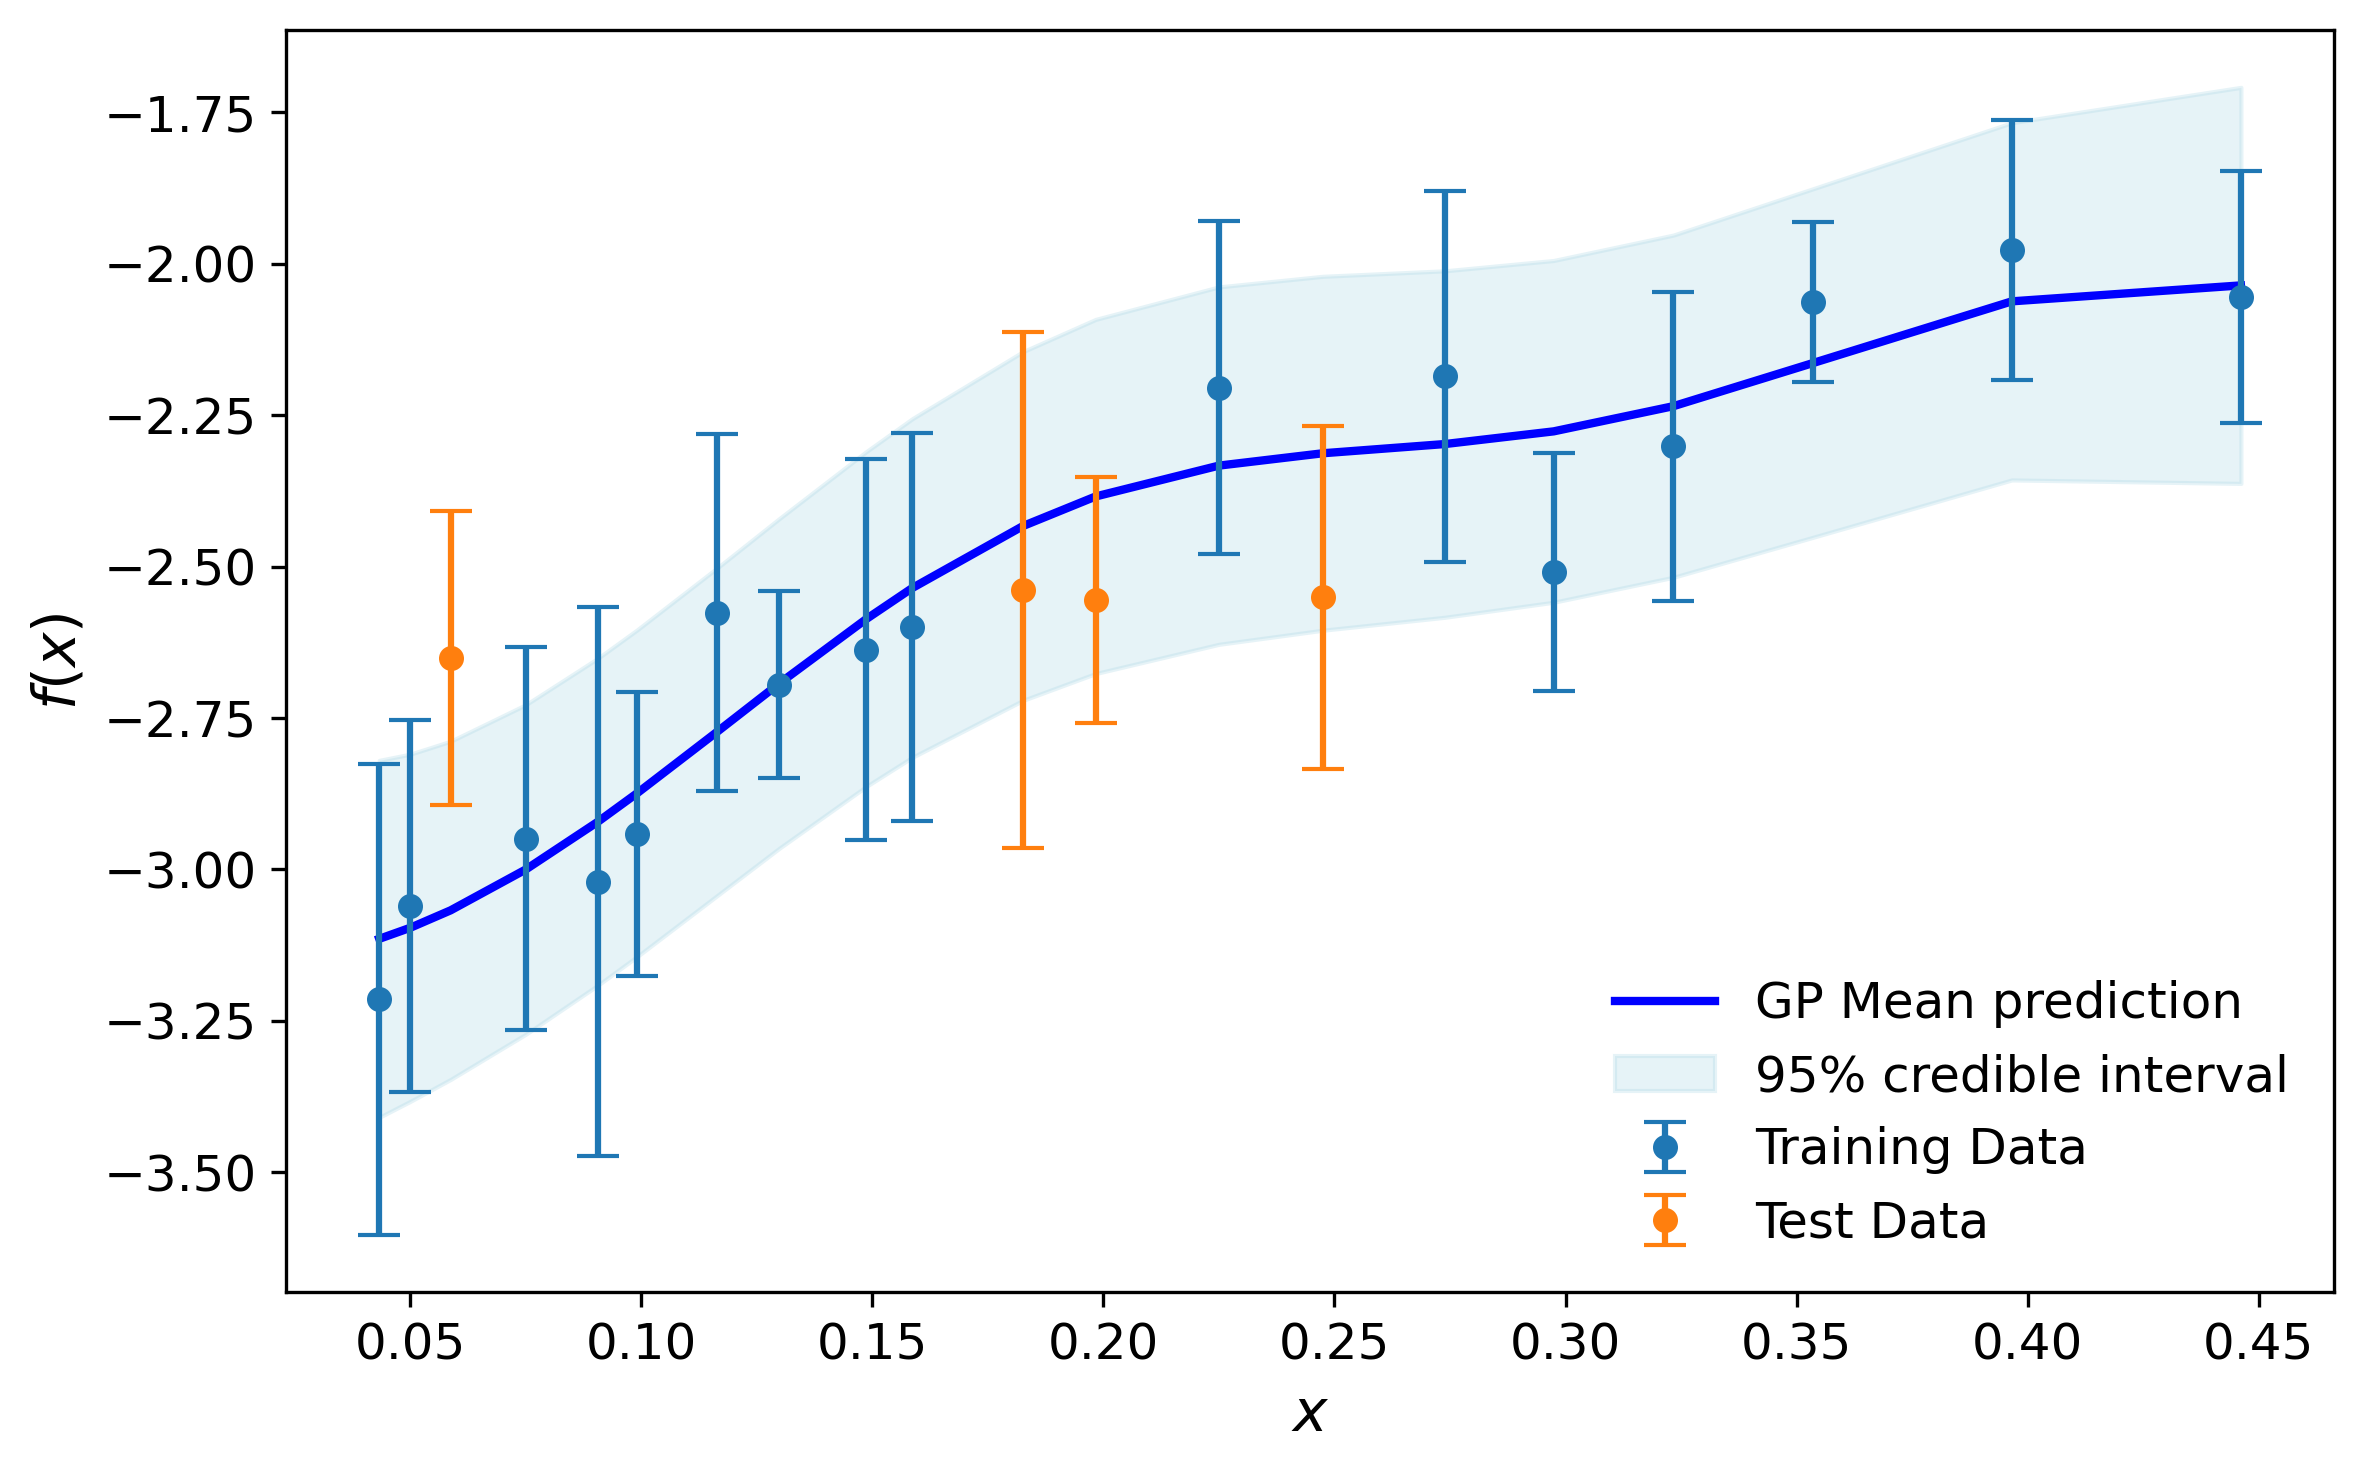
\includegraphics[width=\textwidth]{LatexPlots/1dplots/GPRwhitekernel.png}
    \end{subfigure}
    \hfill
    \begin{subfigure}[b]{0.3\textwidth}
        \centering
        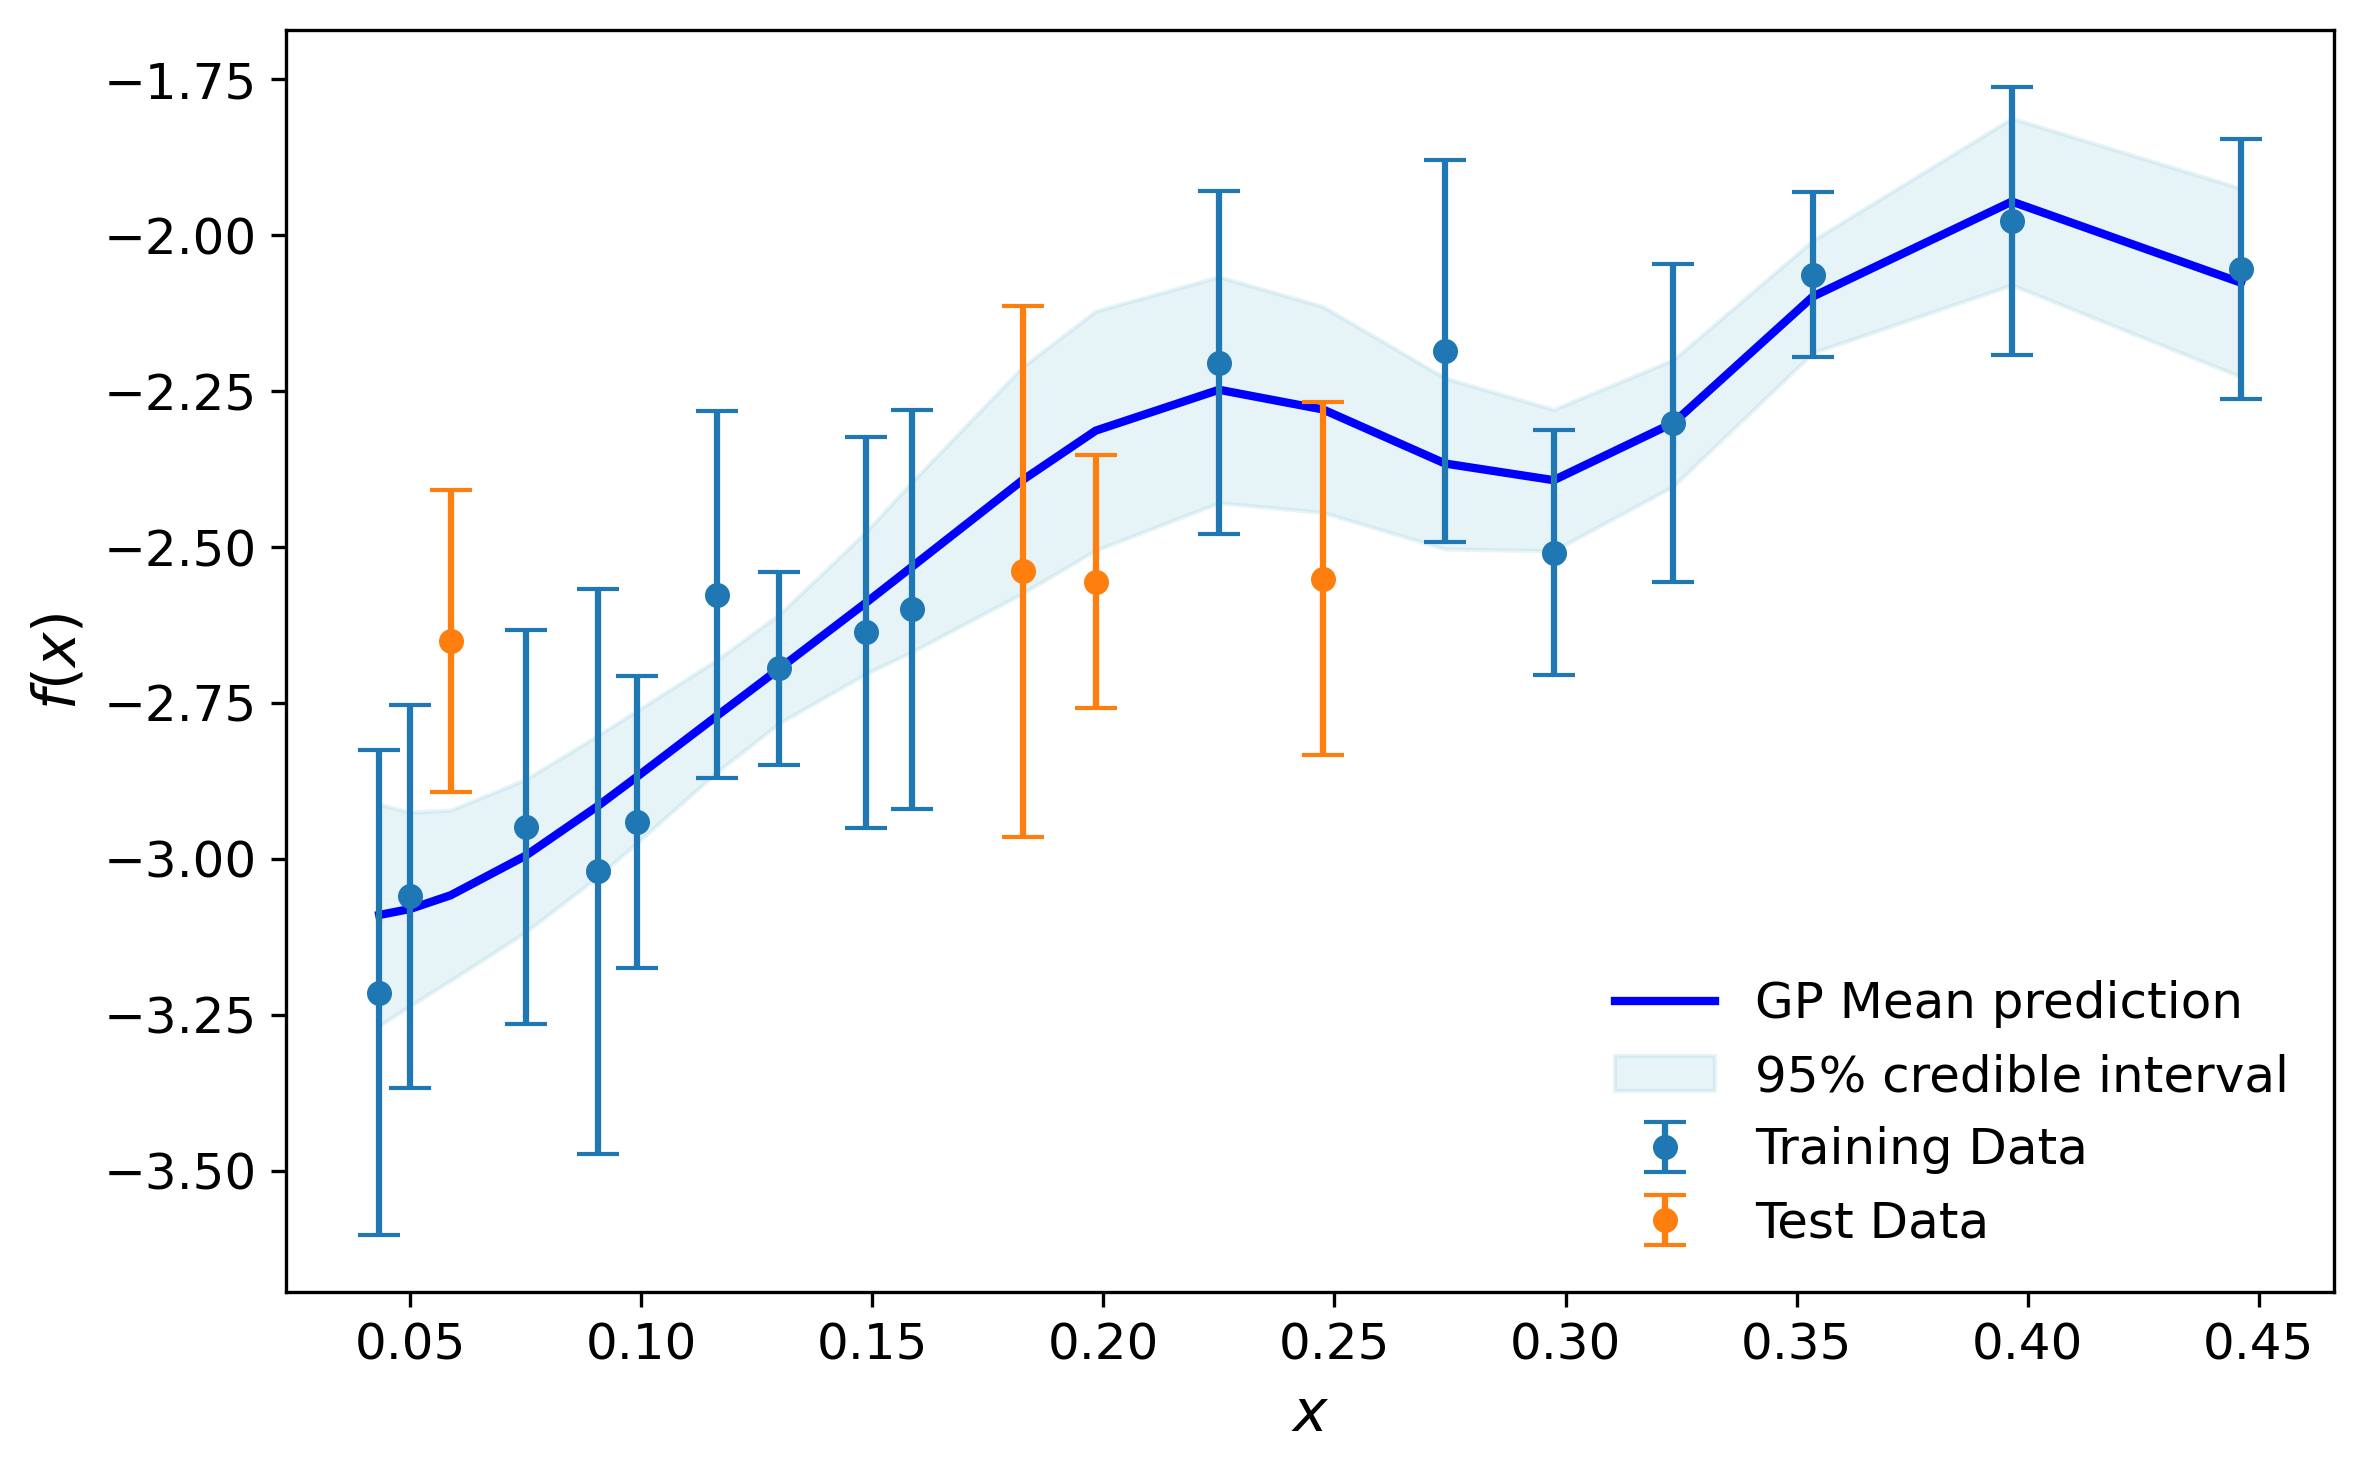
\includegraphics[width=\textwidth]{LatexPlots/1dplots/GPRerror2.png}
    \end{subfigure}
    \hfill
    \begin{subfigure}[b]{0.3\textwidth}
        \centering
        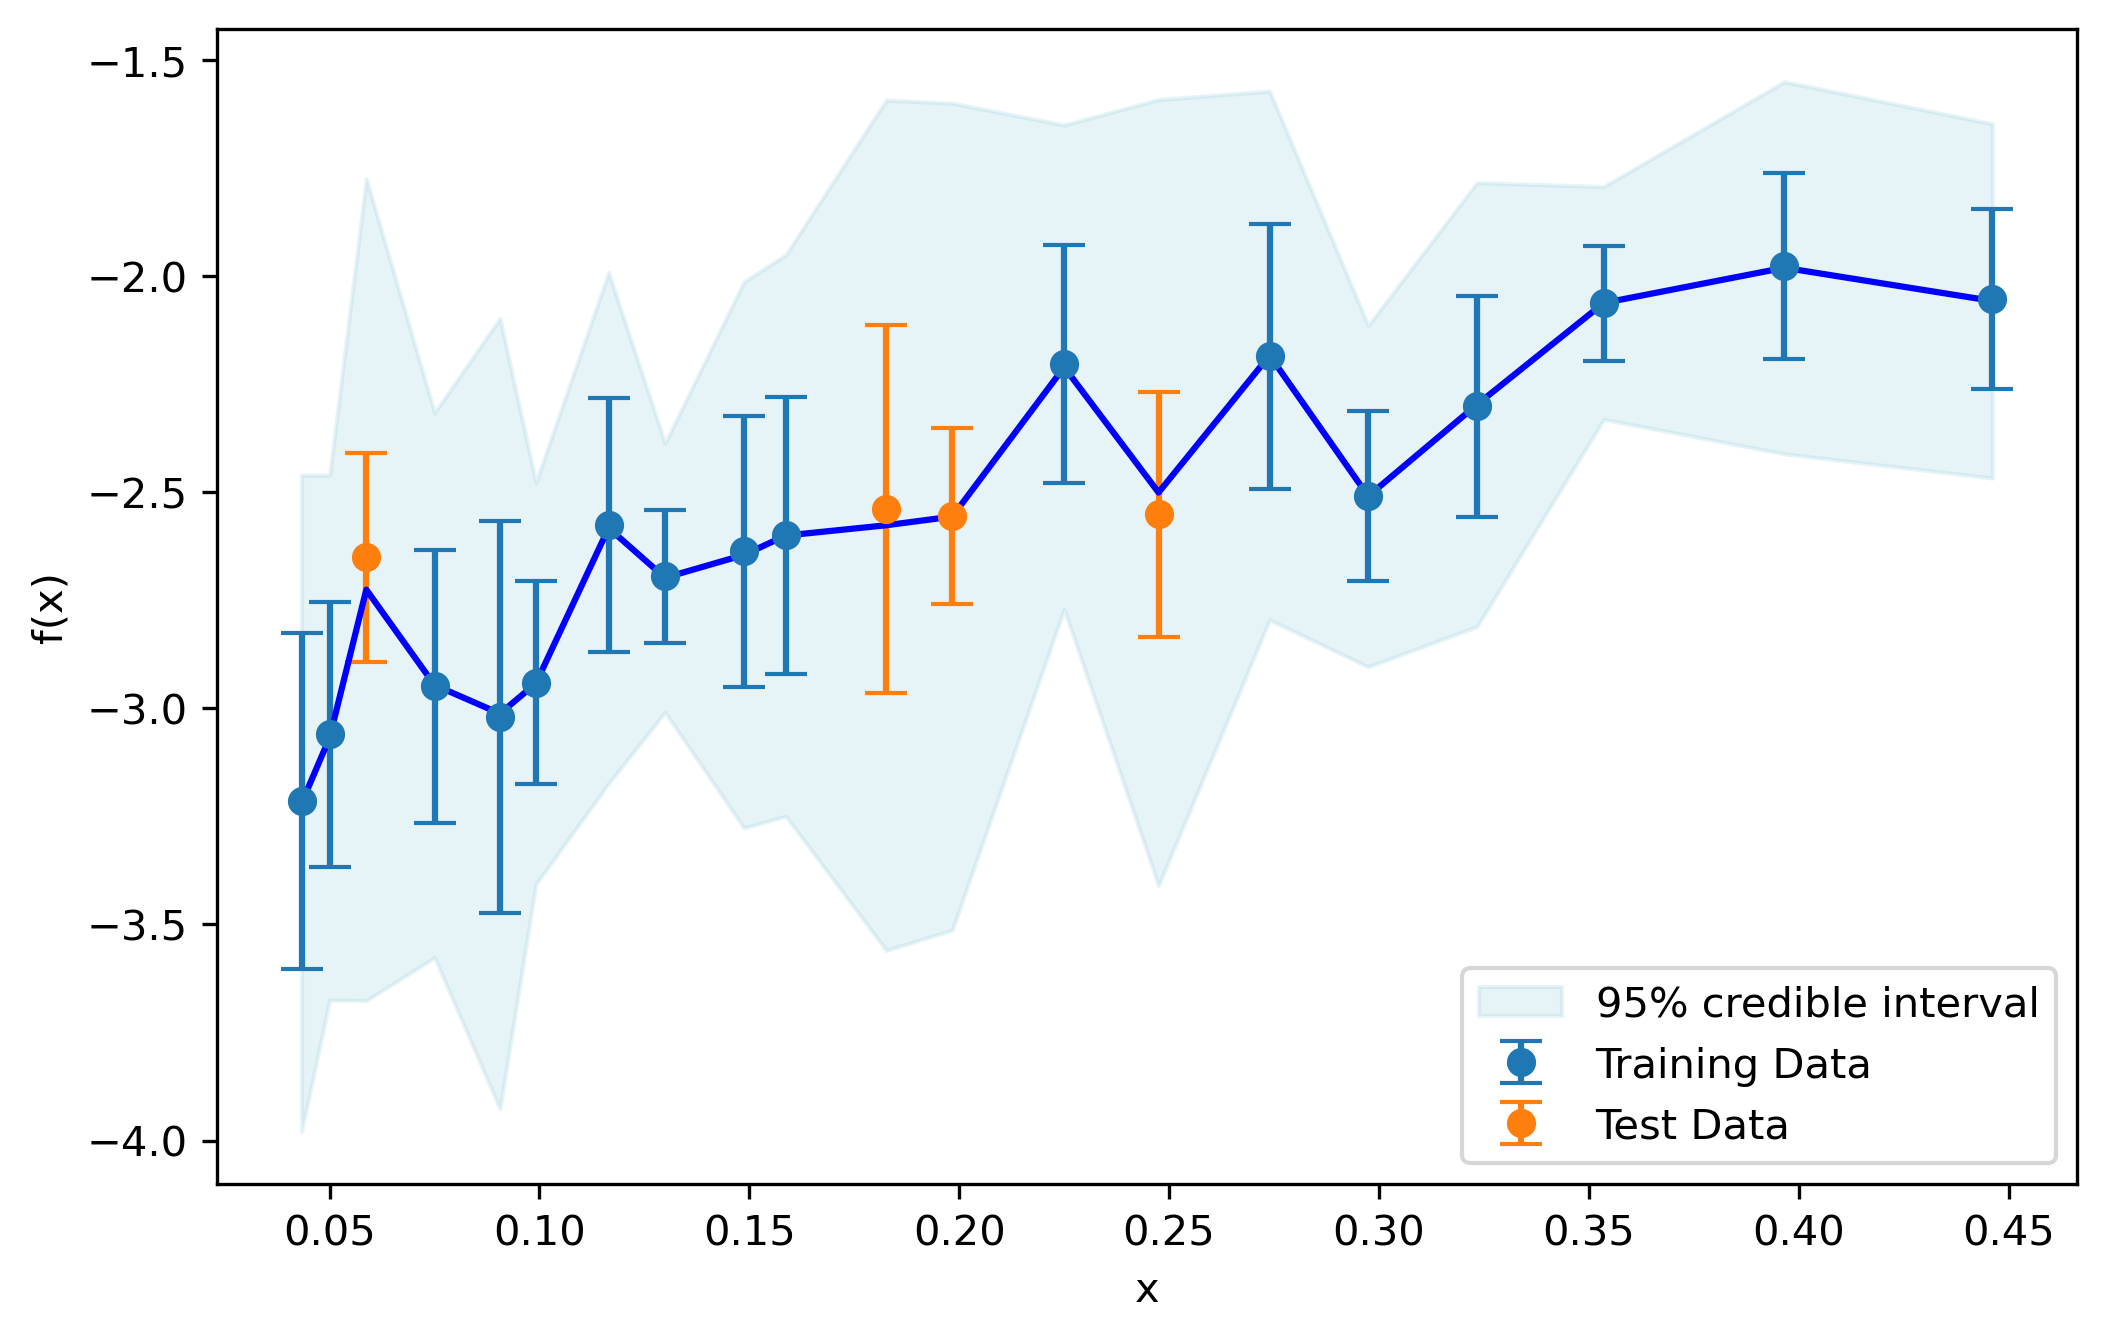
\includegraphics[width=\textwidth]{LatexPlots/1dplots/averagemontecarlosample.png}
    \end{subfigure}
    \caption{
    Left: A white kernel is used to add the noise as a hyper-parameter which is optimised (homoscedastic noise). 
    Middle: We update our covariance function with the true variance at the training points (heteroscedastic noise). 
    Right: Result of Monte Carlo sampling of normally distributed noise at each training point (heteroscedastic noise).
    }
\end{figure}

\textcolor{red}{Add a justification as to the shapes. Why the larger and different confidence intervals}


\subsection{Hyper-parameters}

\bigskip

\noindent
Having now incorporated both prior structure (via kernels) and observational noise, the next step is to fine-tune the model by optimizing its hyperparameters—such as the kernel lengthscale, amplitude, and noise variance—based on the observed data.
Lets examine how the choice of these hyper-parameters effect our mean and our 95 \% credible interval

\begin{figure}[H]
    \centering

    \begin{subfigure}[b]{0.8\textwidth}
        \centering
        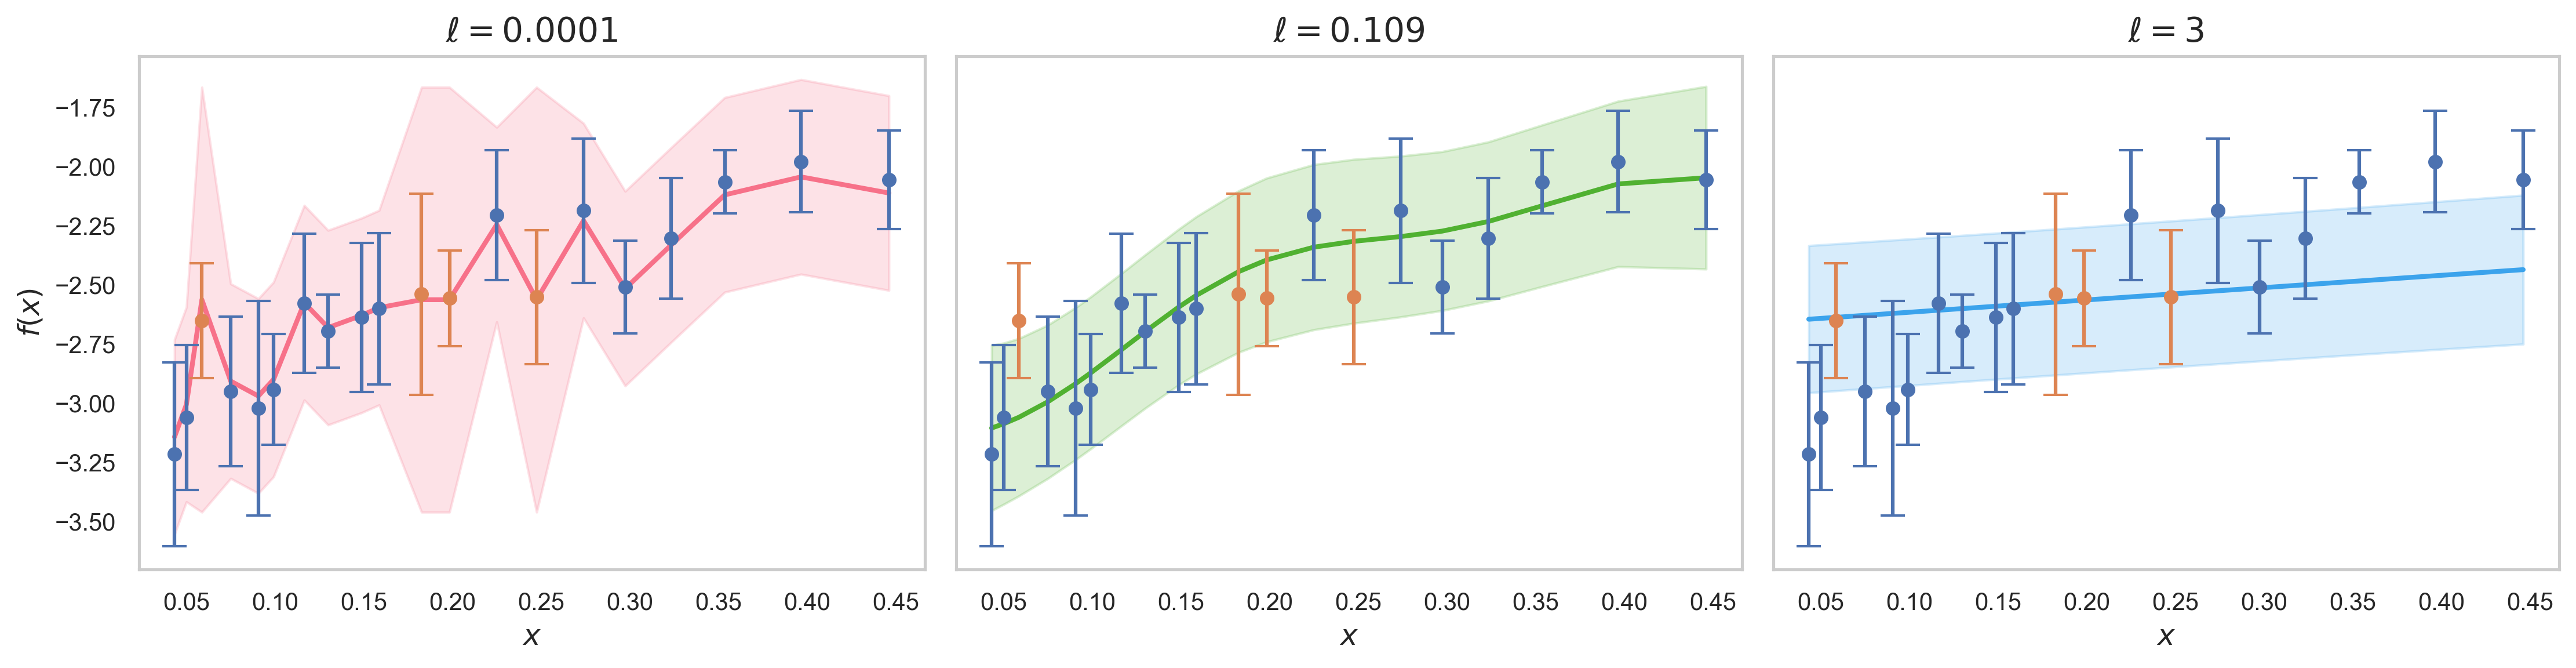
\includegraphics[width=\textwidth]{LatexPlots/1dplots/RBFlengthparam.png}
    \end{subfigure}

    \begin{subfigure}[b]{0.8\textwidth}
        \centering
        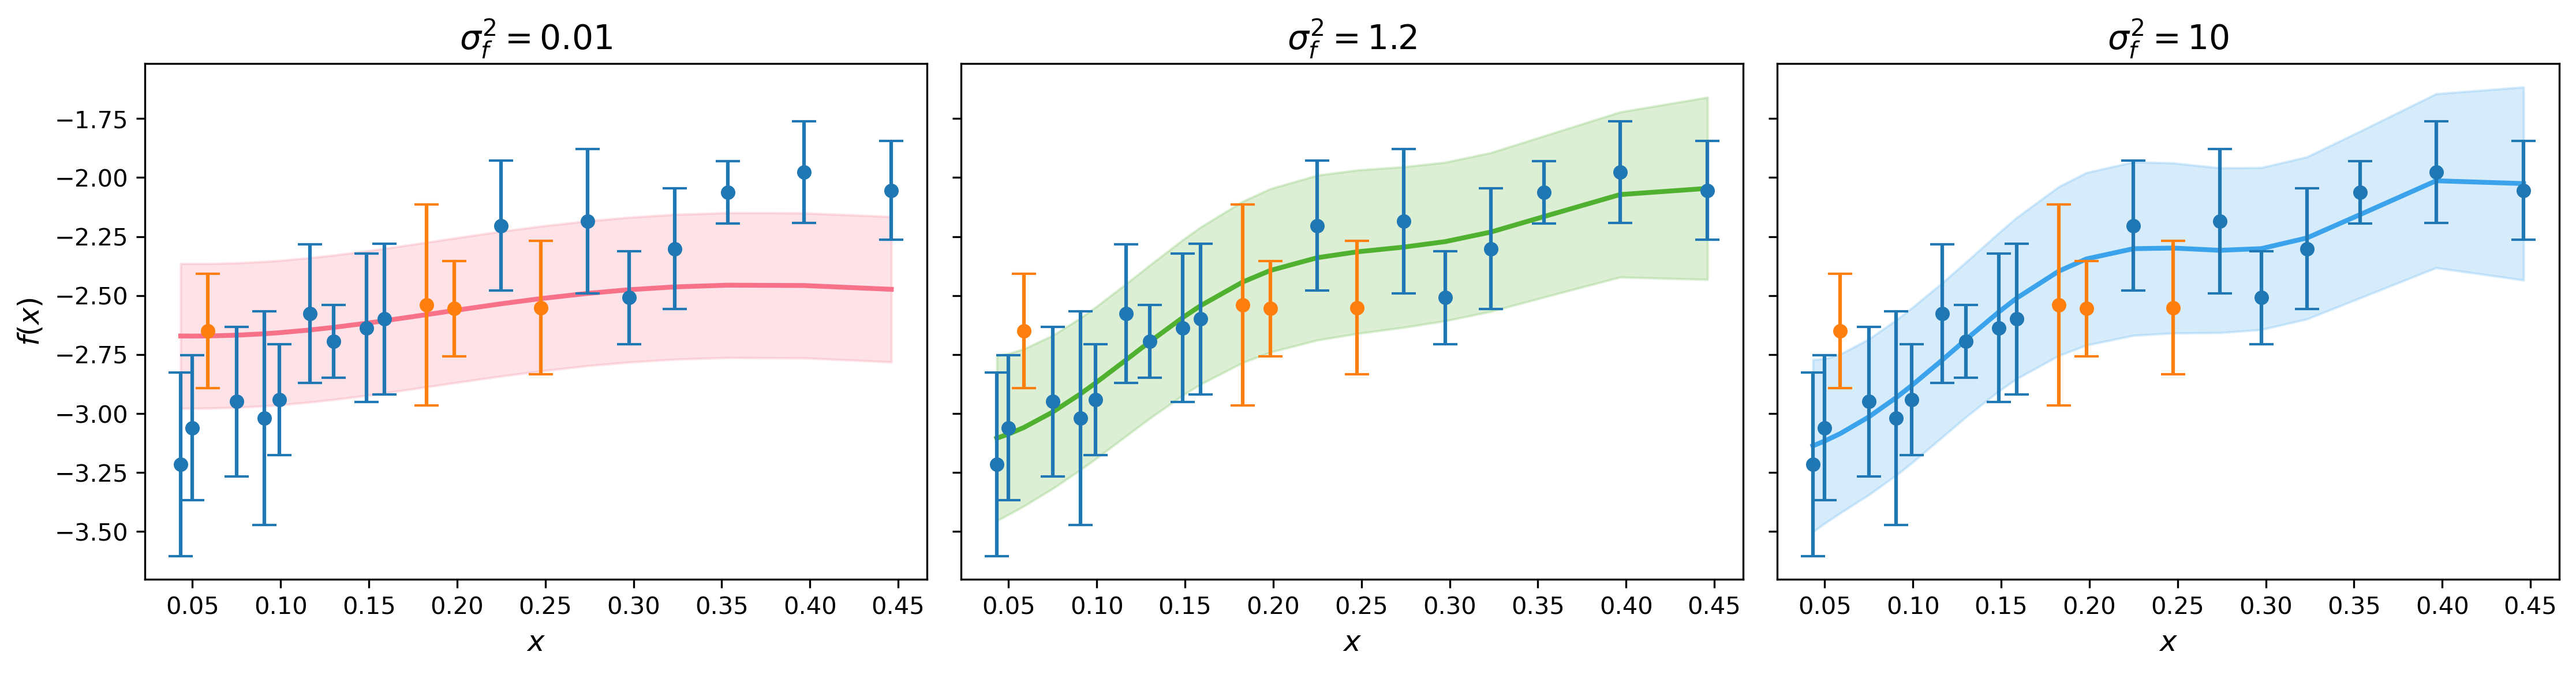
\includegraphics[width=\textwidth]{LatexPlots/1dplots/RBFvarparam.png}
    \end{subfigure}

    \begin{subfigure}[b]{0.8\textwidth}
        \centering
        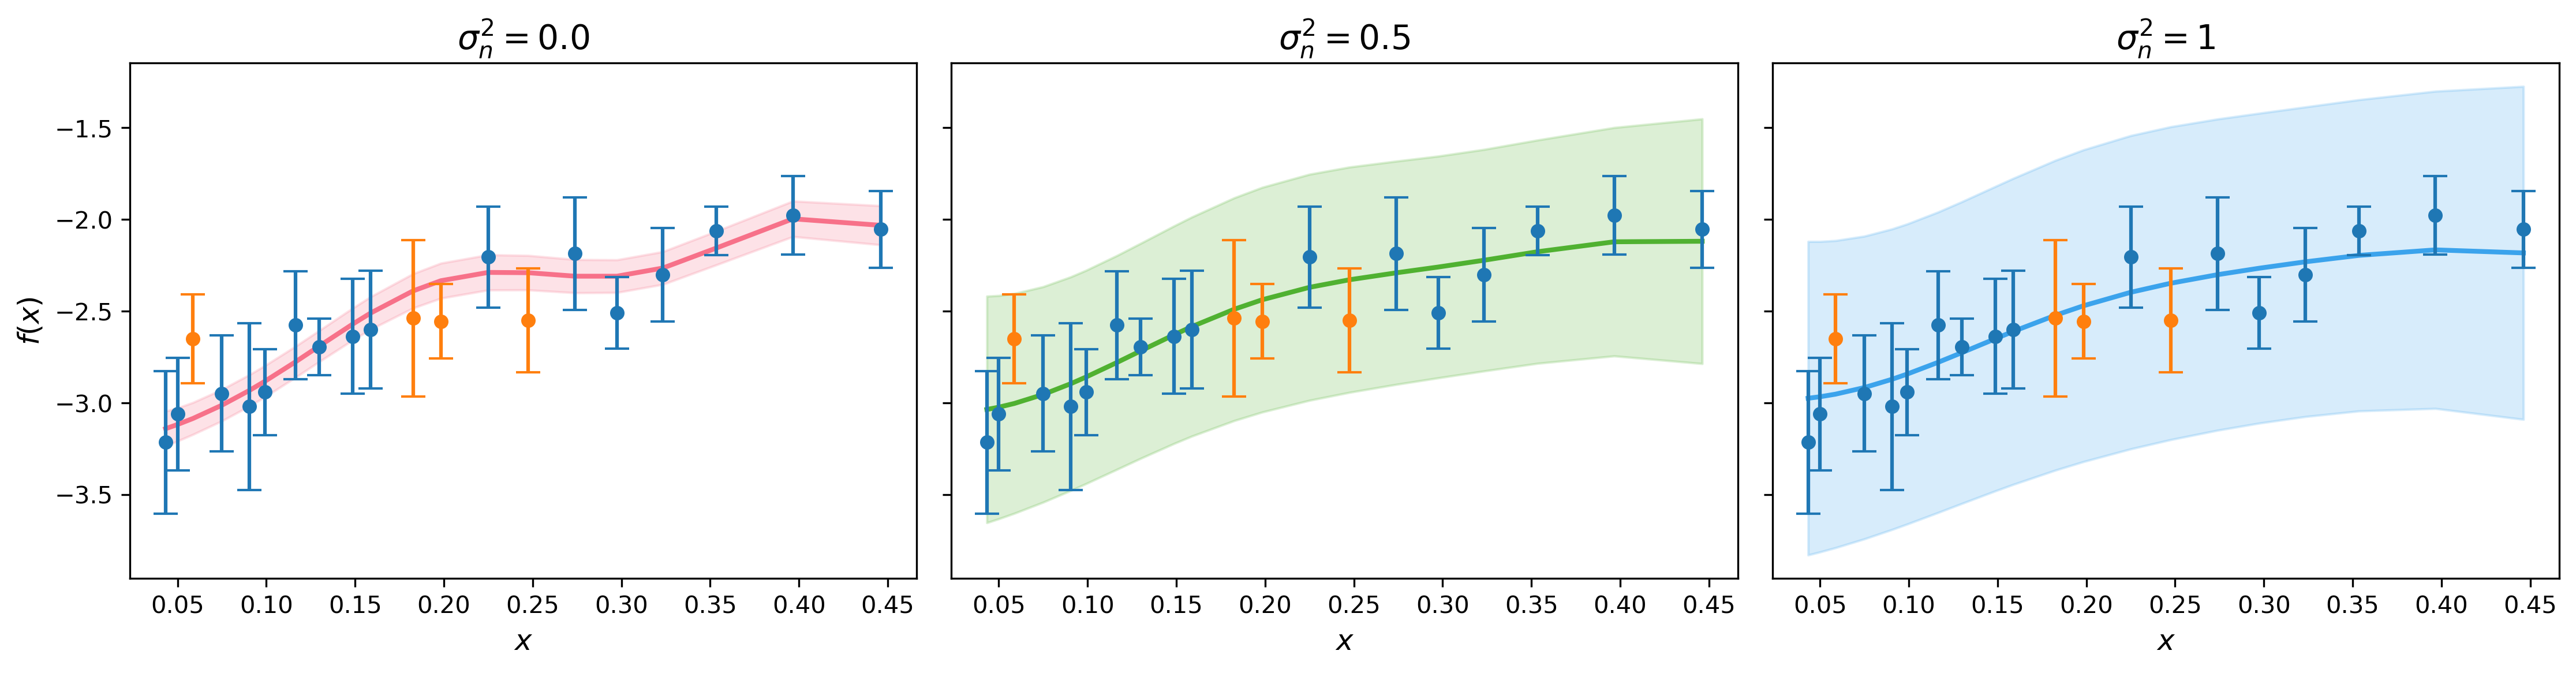
\includegraphics[width=\textwidth]{LatexPlots/1dplots/RBFnoiseparam.png}
    \end{subfigure}

    \caption{This figure outlines the effect of different RBF kernel hyperparameters on Gaussian Process Regression predictions.For each graph the mean is plotted along with the 95\%
    credible region. Each hyper-parameter is set at $\ell=0.109$, $\sigma_f^2 =1.2$ and $\sigma_n^2 = 0.15$ unless explicitly changed}
    \label{figure: Effect of Hyper-parameters}
\end{figure}


\textcolor{red}{ Above graph is misaligned}

\noindent
It is evident that the choice of kernel hyperparameters has a significant impact on the shape of the posterior mean and its uncertainty.
The RBF kernel with noise is given by:
\[
k(x, x') = \sigma_f^2 \exp\left( -\frac{(x - x')^2}{2\ell^2} \right) + \sigma_n^2 I,
\]
where $\ell$ controls the length scale, $\sigma_f^2$ represents the signal variance, and $\sigma_n^2$ denotes the noise level.

\noindent
From Figure~\ref{figure: Effect of Hyper-parameters}, we observe that a very small length scale $\ell \approx 0$ leads to overfitting:
the GP closely tracks the training data, with sharp fluctuations between points. This occurs because the kernel's covariance rapidly decays with distance,
making function values at different inputs nearly uncorrelated unless they are extremely close. As a result, the model fits the noise and exhibits a jagged appearance.
In contrast, a large length scale such as $\ell \approx 3$ causes over-smoothing. Distant points remain highly correlated,
producing a nearly linear mean function that fails to capture local variations. A moderate length scale ($\ell = 0.109$ in this case)
provides a balance—producing a smooth yet flexible mean function that captures trends in the data without overfitting.

\noindent
Regarding the signal variance $\sigma_f^2$, we find that a very small value (e.g., $\sigma_f^2 \approx 0.01$) causes the GP mean to flatten,
as the prior assumes the function to vary very little. As the variance increases (e.g., $\sigma_f^2 = 1.2$ and $\sigma_f^2 = 10$), the credible intervals widen slightly,
but the overall mean function shape remains relatively stable. This suggests that posterior inference over $\sigma_f^2$ may exhibit considerable uncertainty, a point we explore further using MCMC sampling in Section \ref{sec: MCMC}.


\noindent
Lastly, varying the noise level $\sigma_n^2$ primarily affects the width of the credible interval, 
while the mean function remains largely unchanged. As $\sigma_n^2$ increases, the model accounts for higher observation noise, 
and uncertainty in the predictions increases accordingly. This relationship appears approximately linear in the visualizations.


\subsubsection{Learning Hyperparameters by Maximising the Log Marginal Likelihood}
\label{sec: hyperparam optimisation}

Now that we have seen how the choice of hyperparameters affects the posterior distribution, we aim to find the optimal hyperparameters that allow the model to best explain the observed data. This is done by maximising the \textit{log marginal likelihood}, as described in \cite{rasmussen2006gaussian}.

\bigskip
\noindent
From Equation~\ref{eq: 4}, we have:
\[
y \sim \mathcal{N}(0, K + \sigma_n^2 I)
\]
where \( K \) is the kernel matrix computed from the training inputs \( X \), and \( \sigma_n^2 \) is the noise variance.

\noindent
This implies that the marginal likelihood (i.e., the probability of the observed outputs \( y \) given the inputs \( X \) and hyperparameters \( \theta \)) is given by the multivariate Gaussian density:
\[
p(y \mid X, \theta) = \frac{1}{(2\pi)^{n/2} |K_y|^{1/2}} \exp\left( -\frac{1}{2} y^\top K_y^{-1} y \right)
\]
where \( K_y = K + \sigma_n^2 I \).

\bigskip

\noindent
Taking the logarithm of this expression yields the \textit{log marginal likelihood}:
\begin{equation}\label{eq: 5}
\log p(y \mid X, \theta) = -\frac{1}{2} y^\top K_y^{-1} y - \frac{1}{2} \log |K_y| - \frac{n}{2} \log 2\pi
\end{equation}

\noindent
Our goal is to maximise this log marginal likelihood with respect to the hyperparameters \( \theta \), which typically includes the kernel lengthscale, signal variance, and noise variance. Once optimal values are found, we can use them to make accurate posterior predictions.



\begin{figure}[H]
    \centering
    \begin{subfigure}[b]{0.4\textwidth}
        \centering
        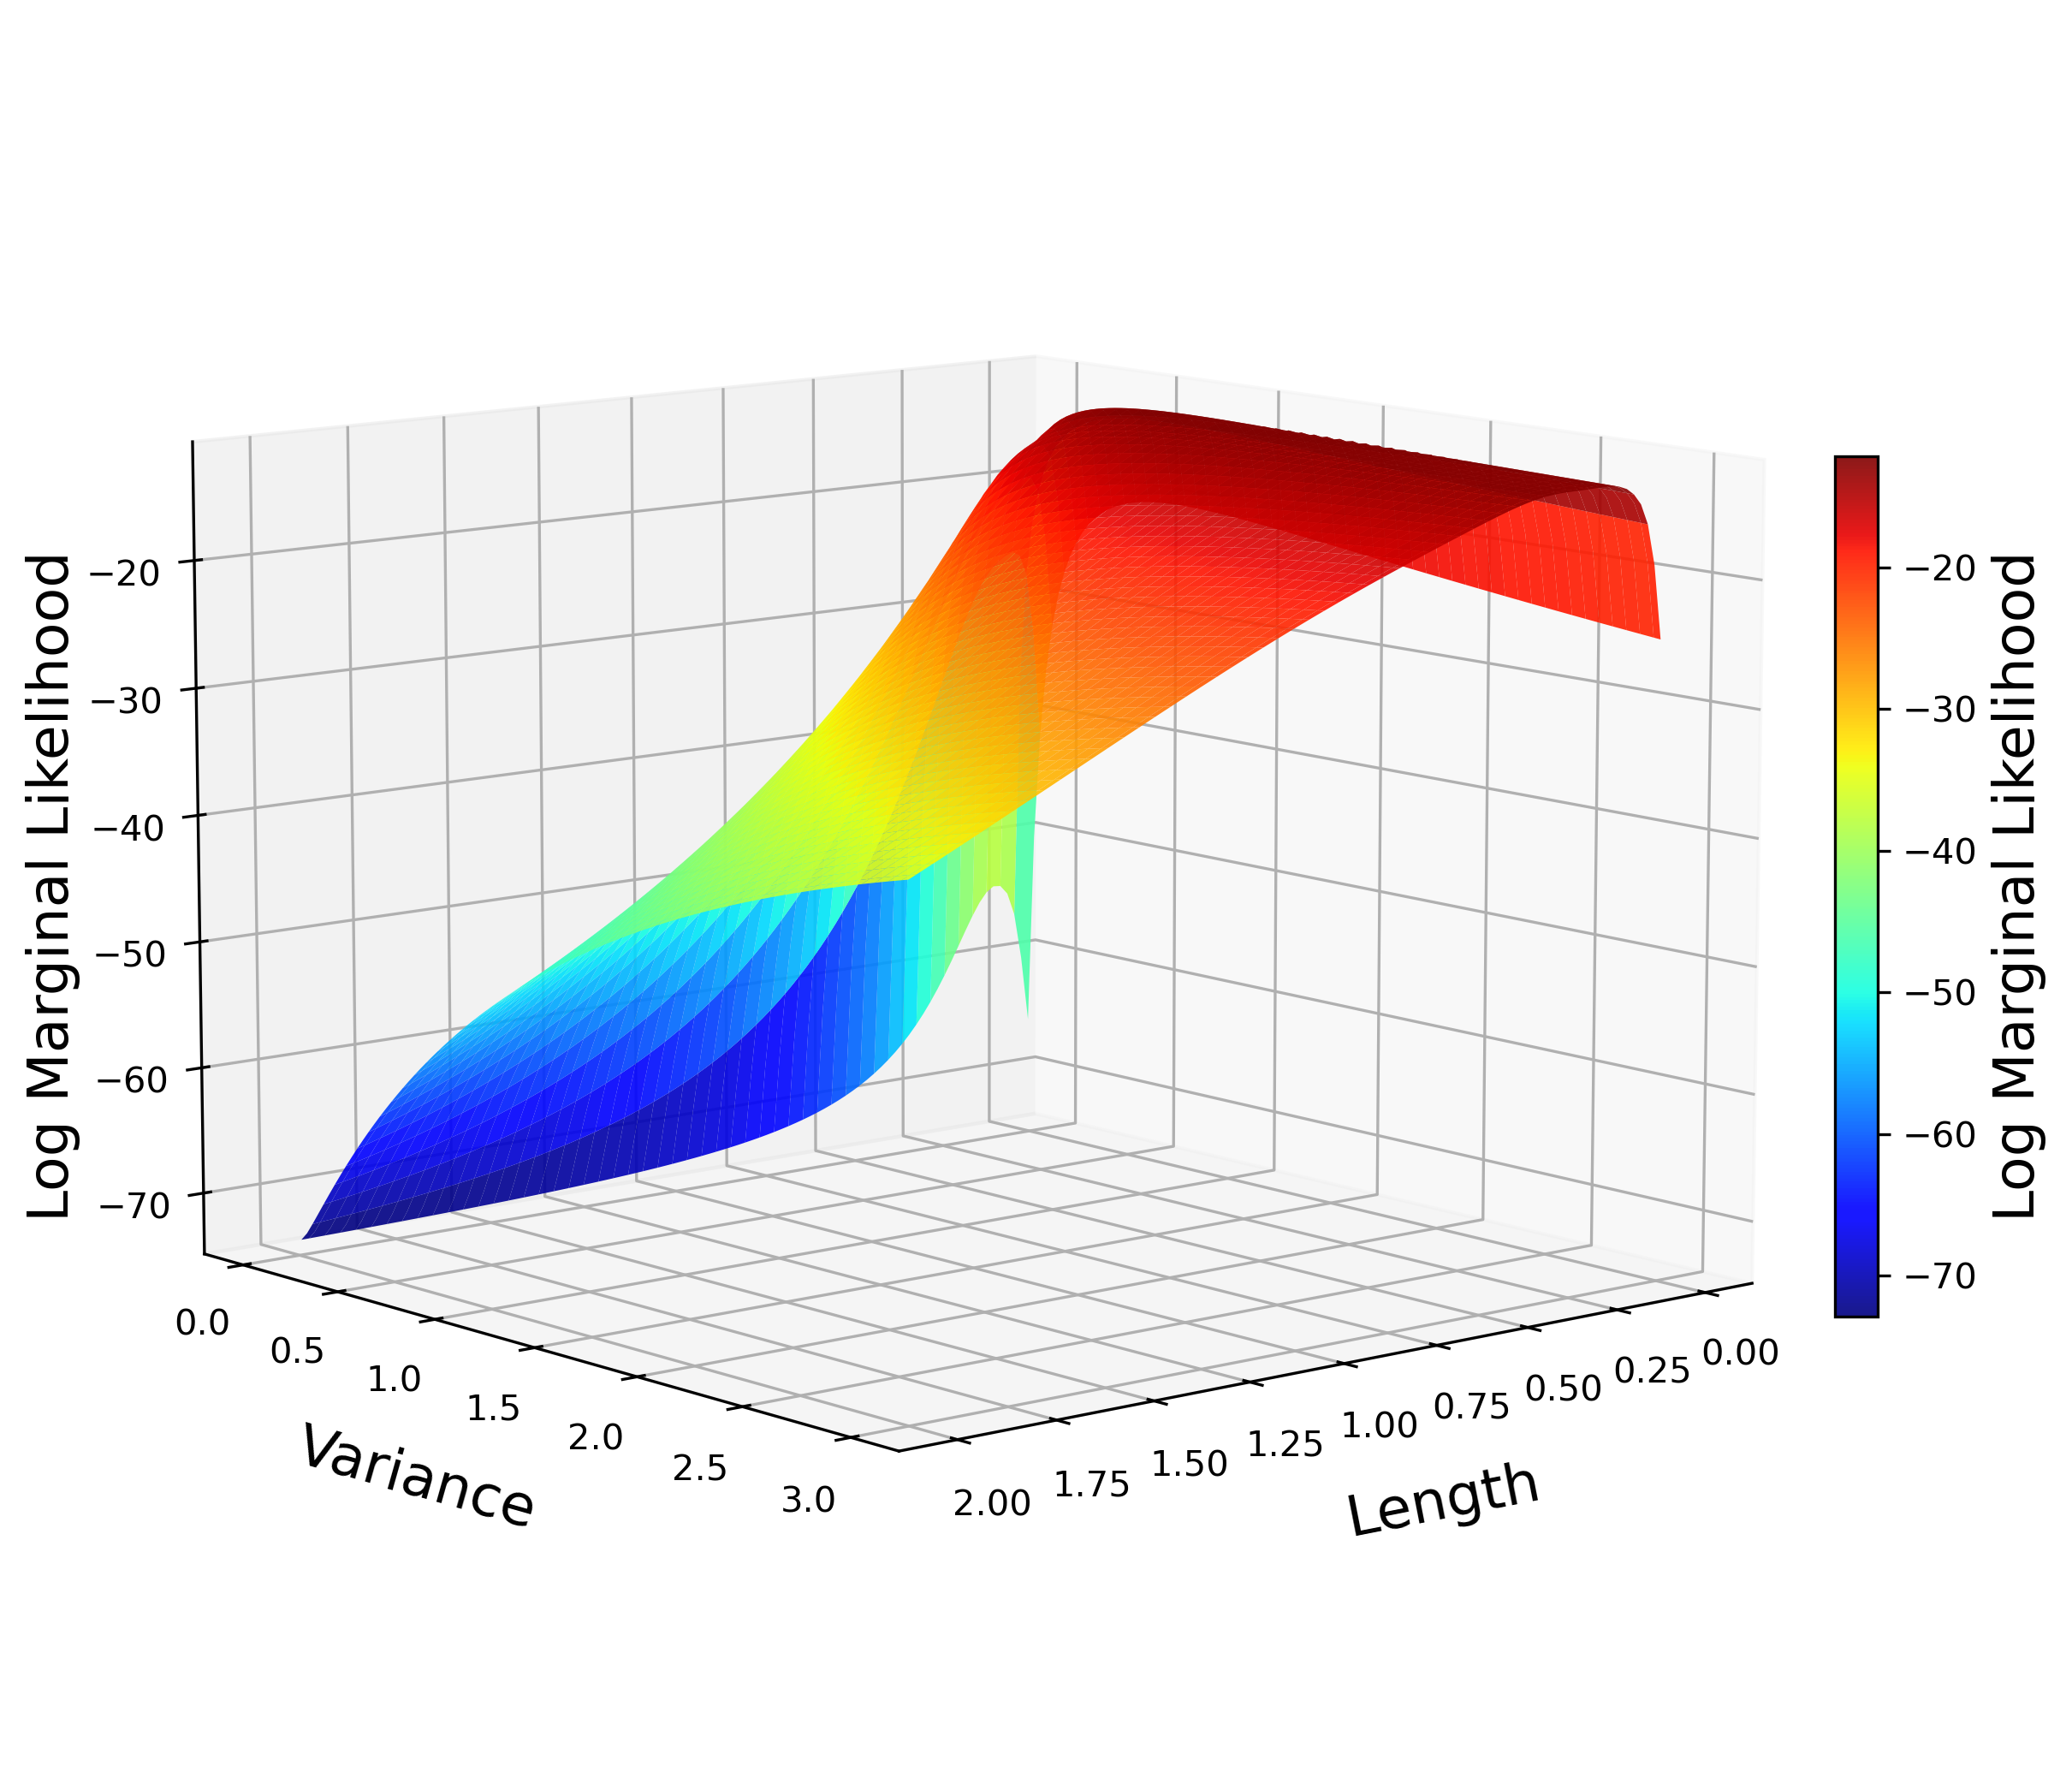
\includegraphics[width=\textwidth]{LatexPlots/1dplots/Variancevslength.png}
    \end{subfigure}
    \hspace{0.05\textwidth}
    \begin{subfigure}[b]{0.4\textwidth}
        \centering
        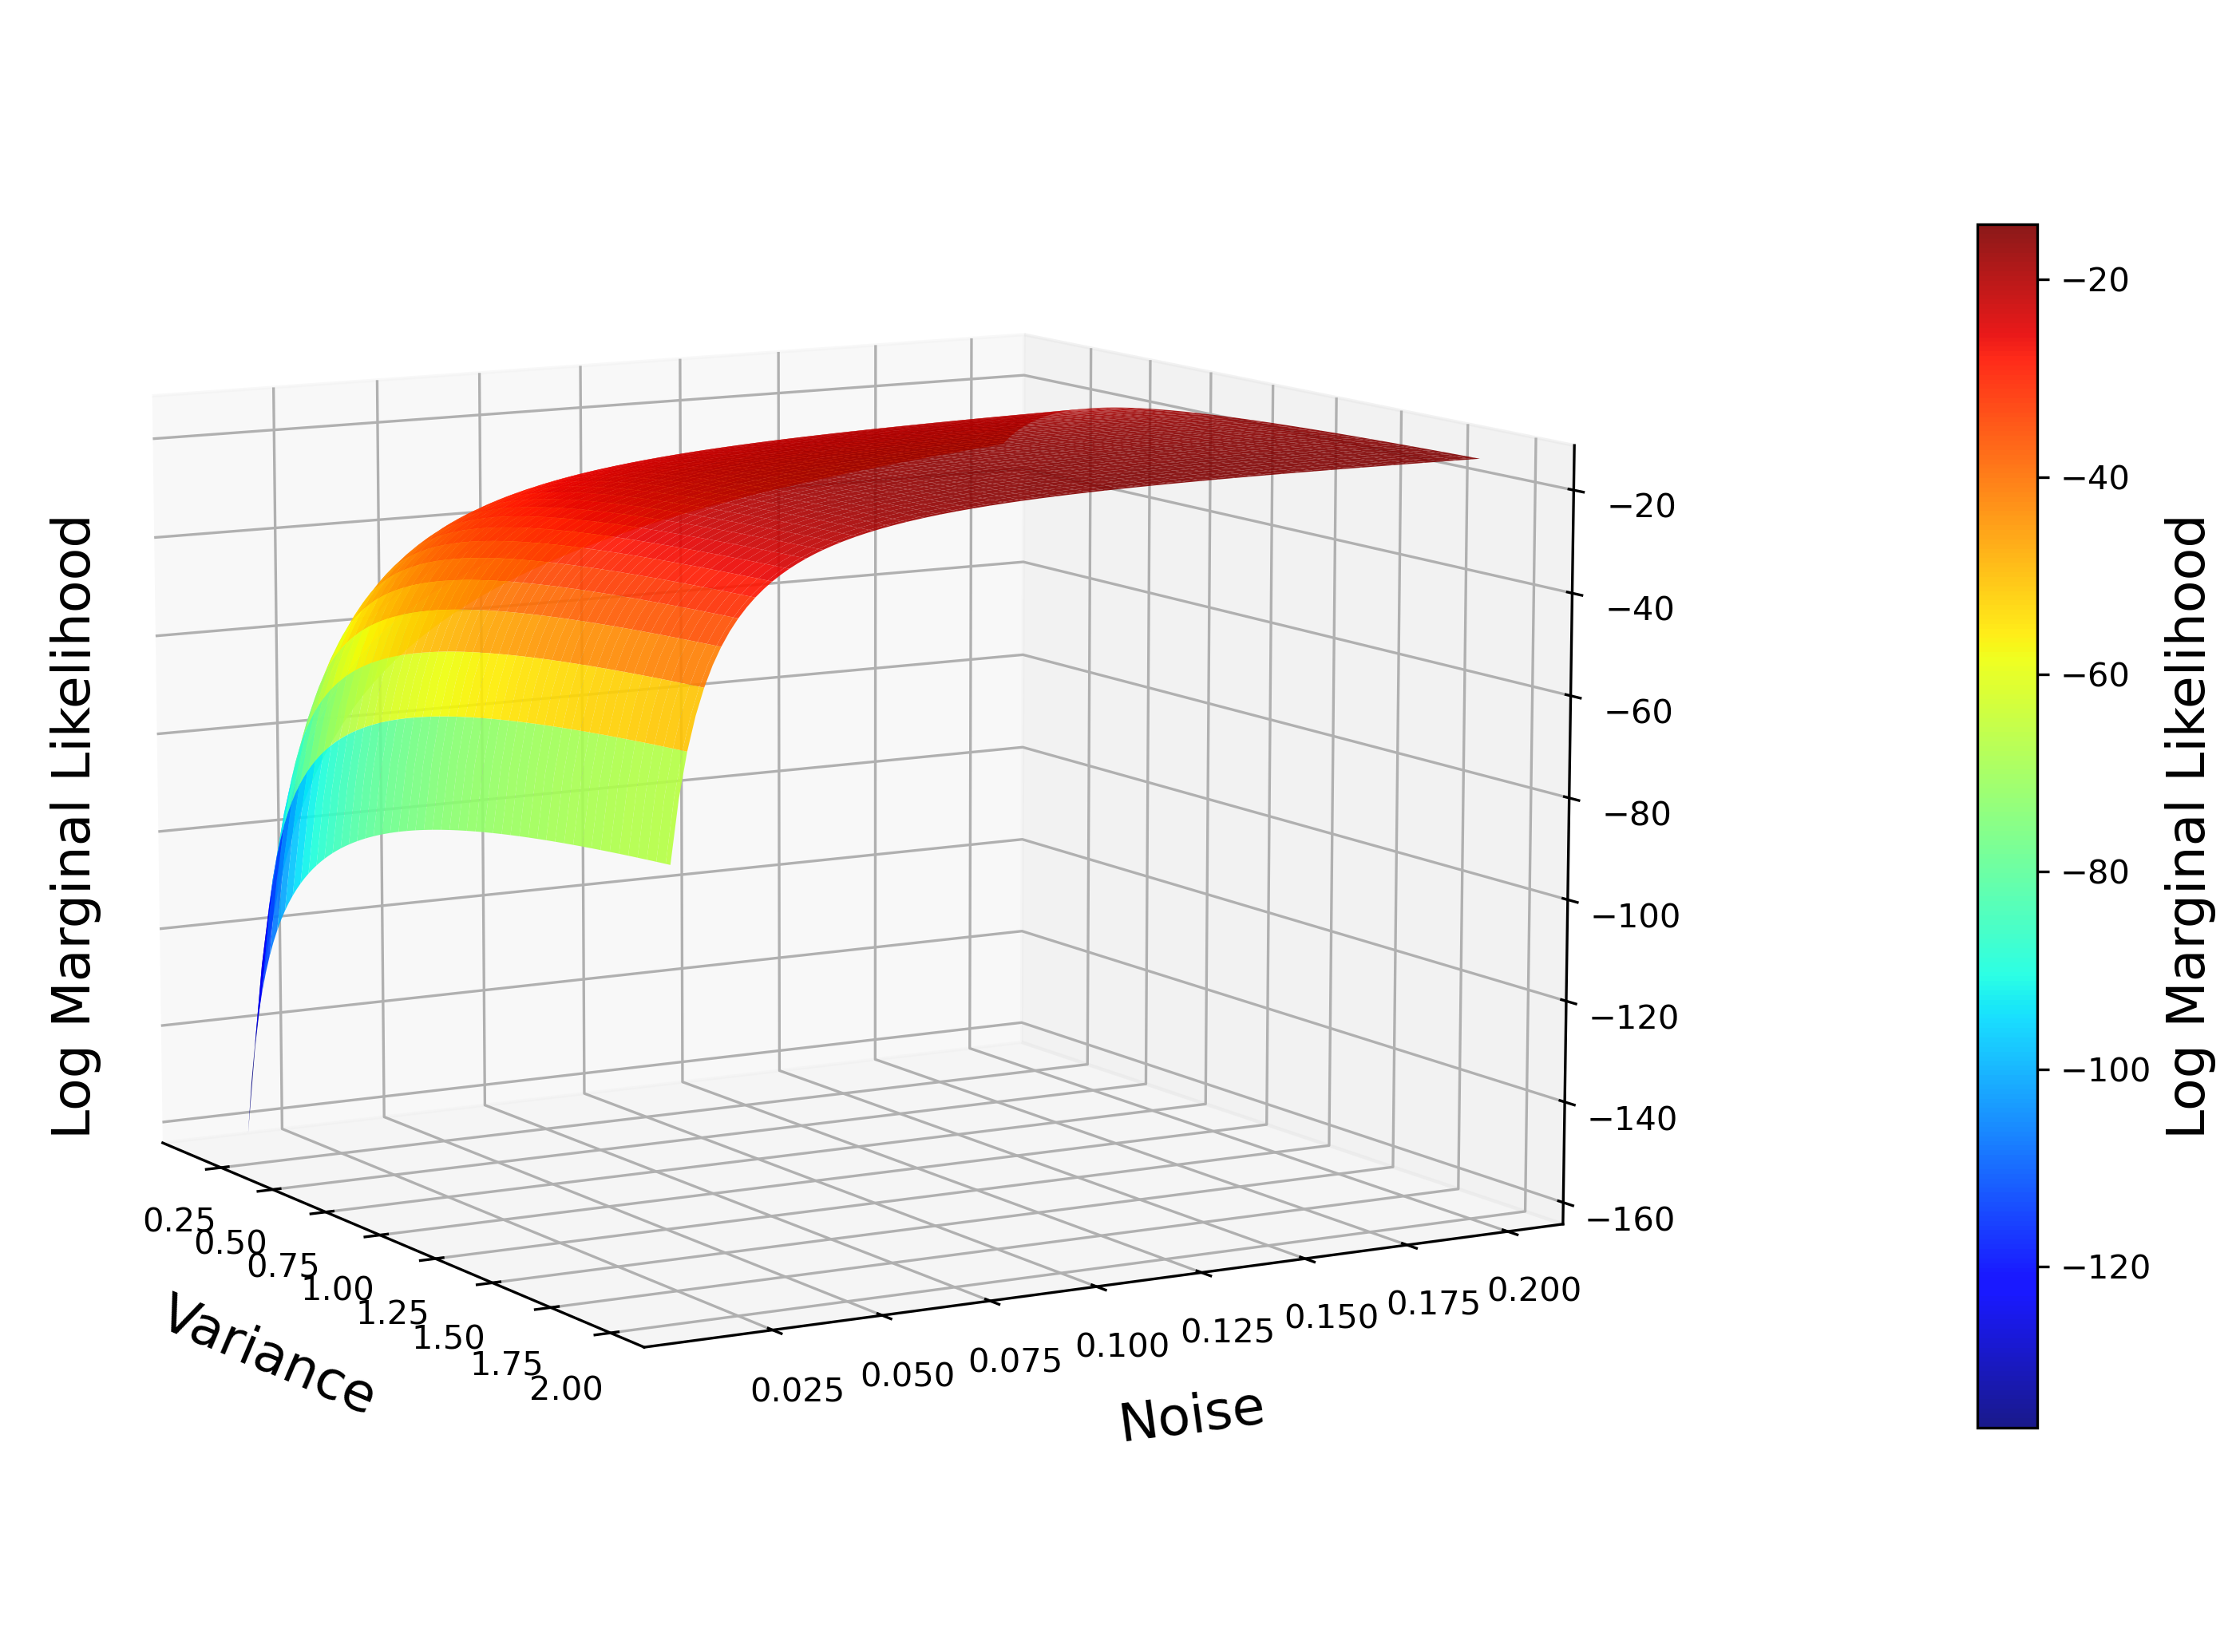
\includegraphics[width=\textwidth]{LatexPlots/1dplots/Variancevsnoise.png}
    \end{subfigure}
    \vspace{0.05em}
    \begin{subfigure}[b]{0.4\textwidth}
        \centering
        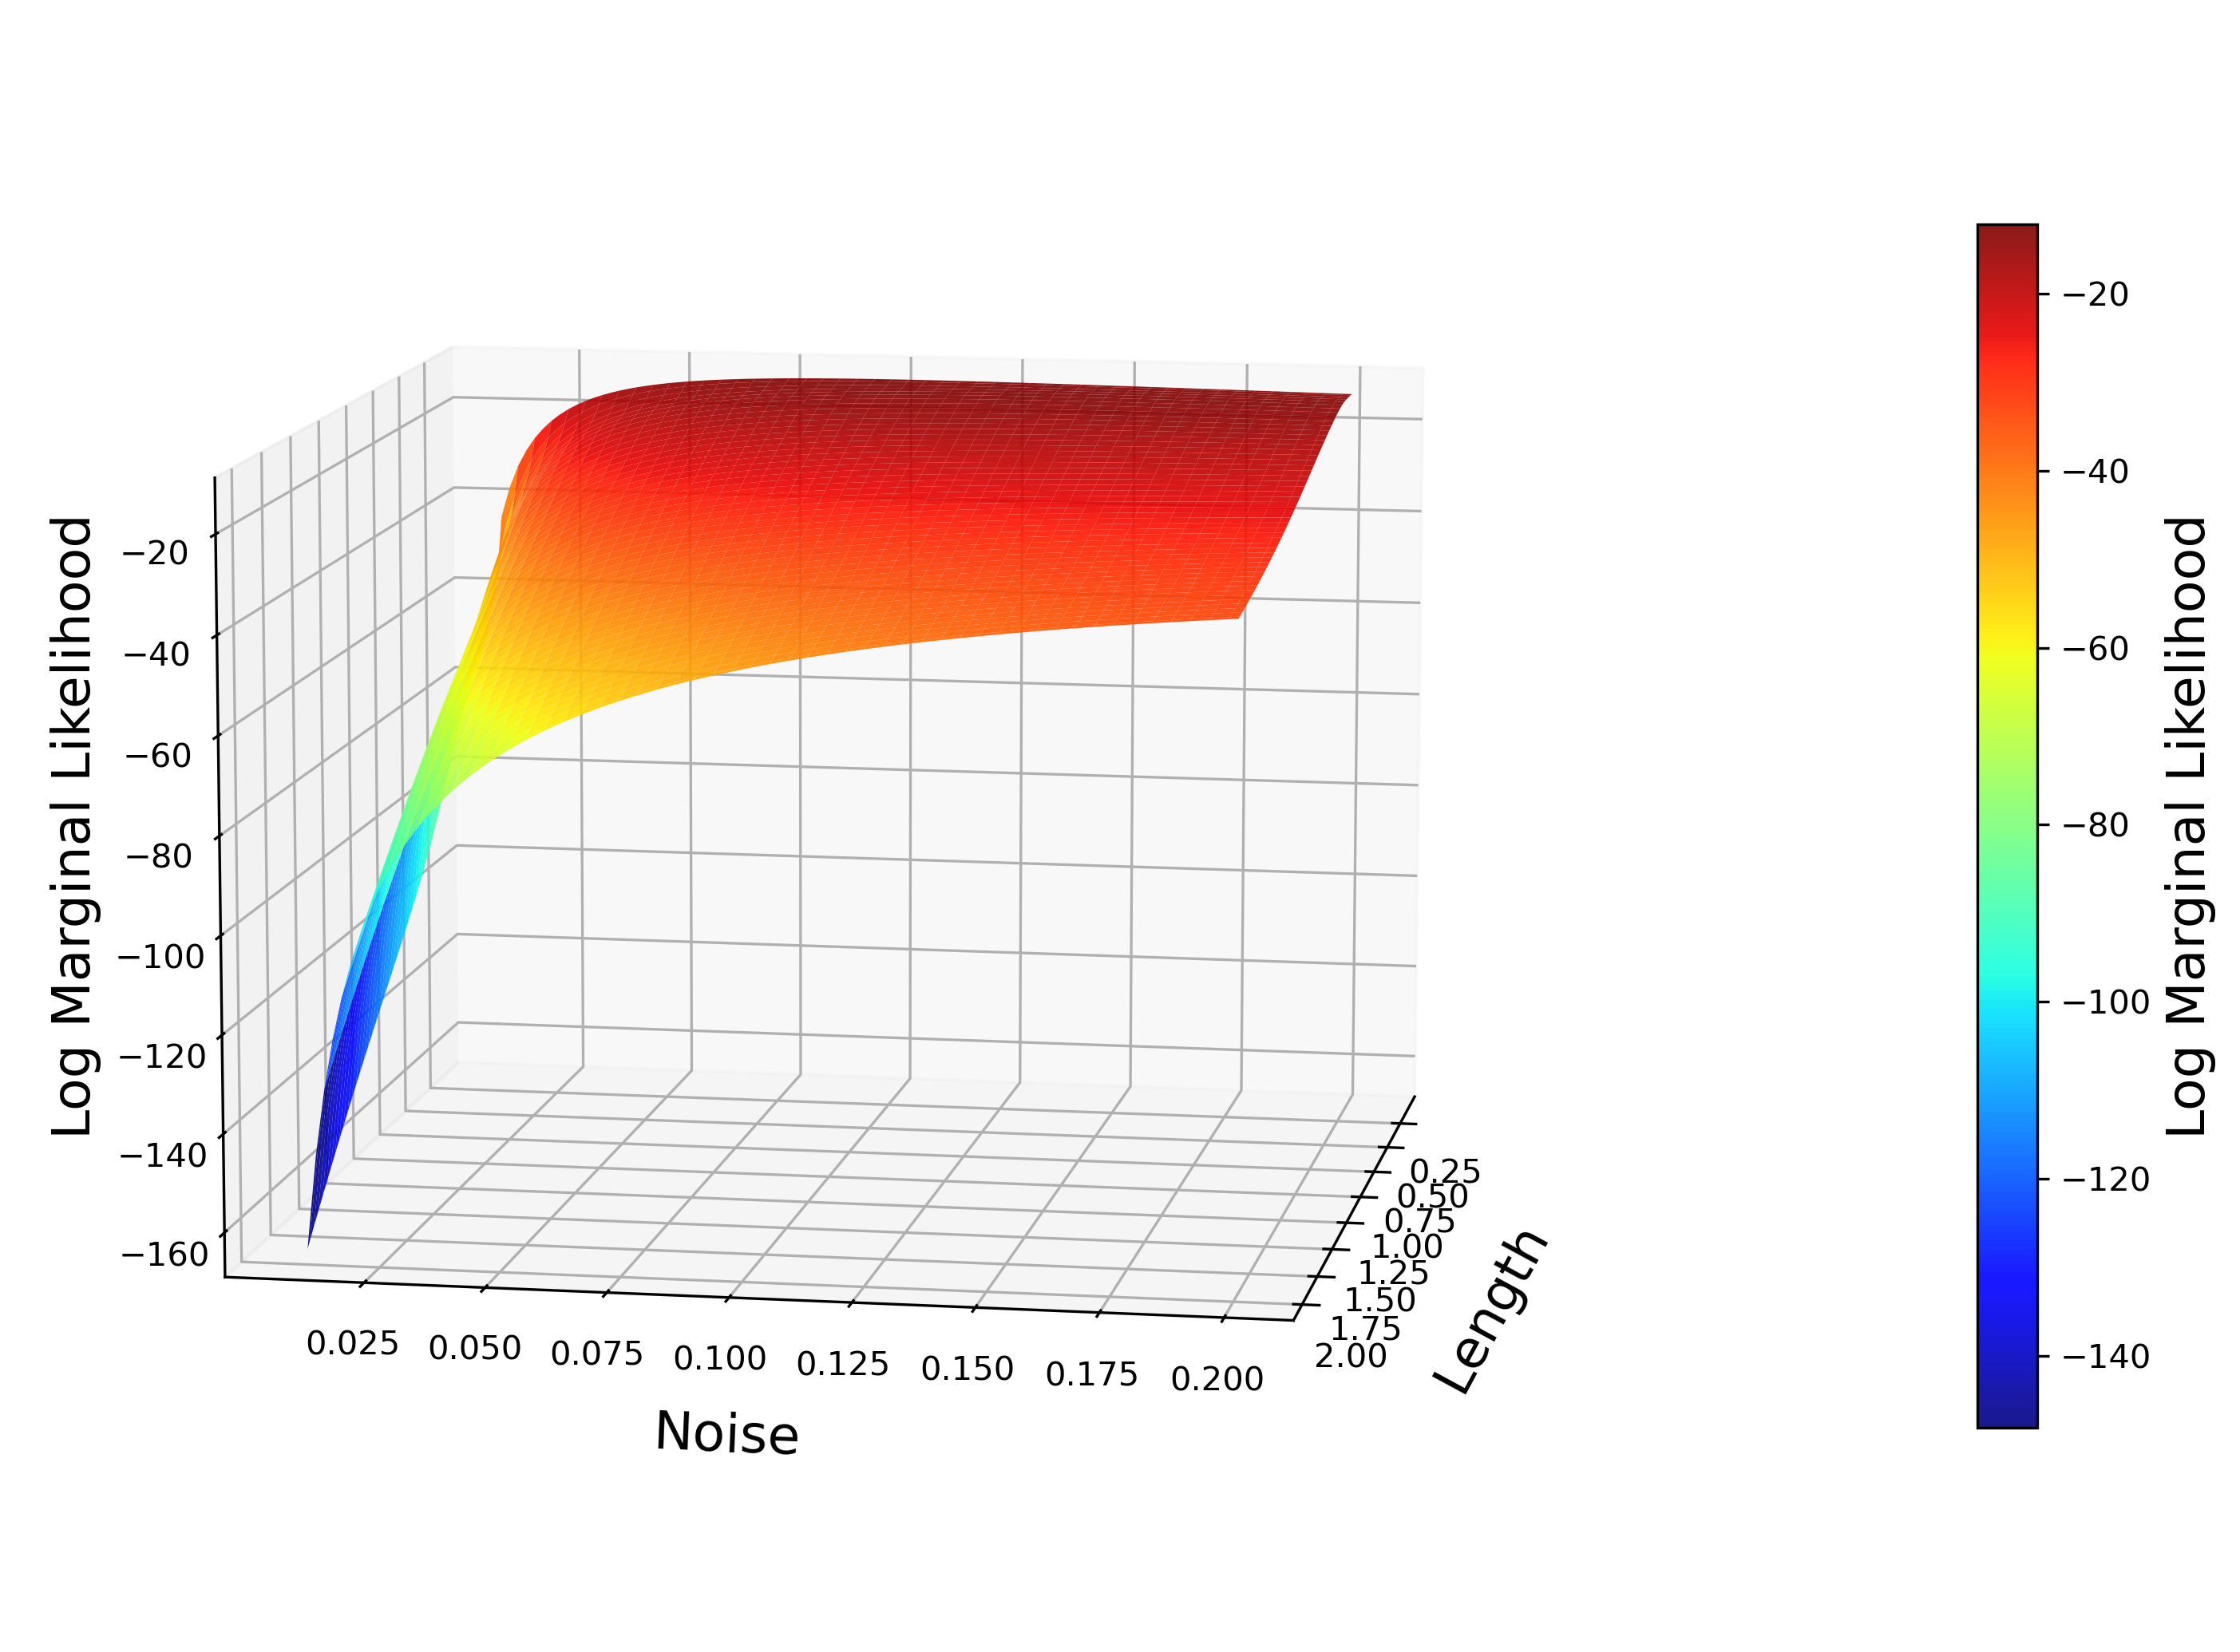
\includegraphics[width=\textwidth]{LatexPlots/1dplots/lengthvsnoise.png}
    \end{subfigure}
    \hspace{0.05\textwidth}
    \begin{subfigure}[b]{0.4\textwidth}
        \centering
        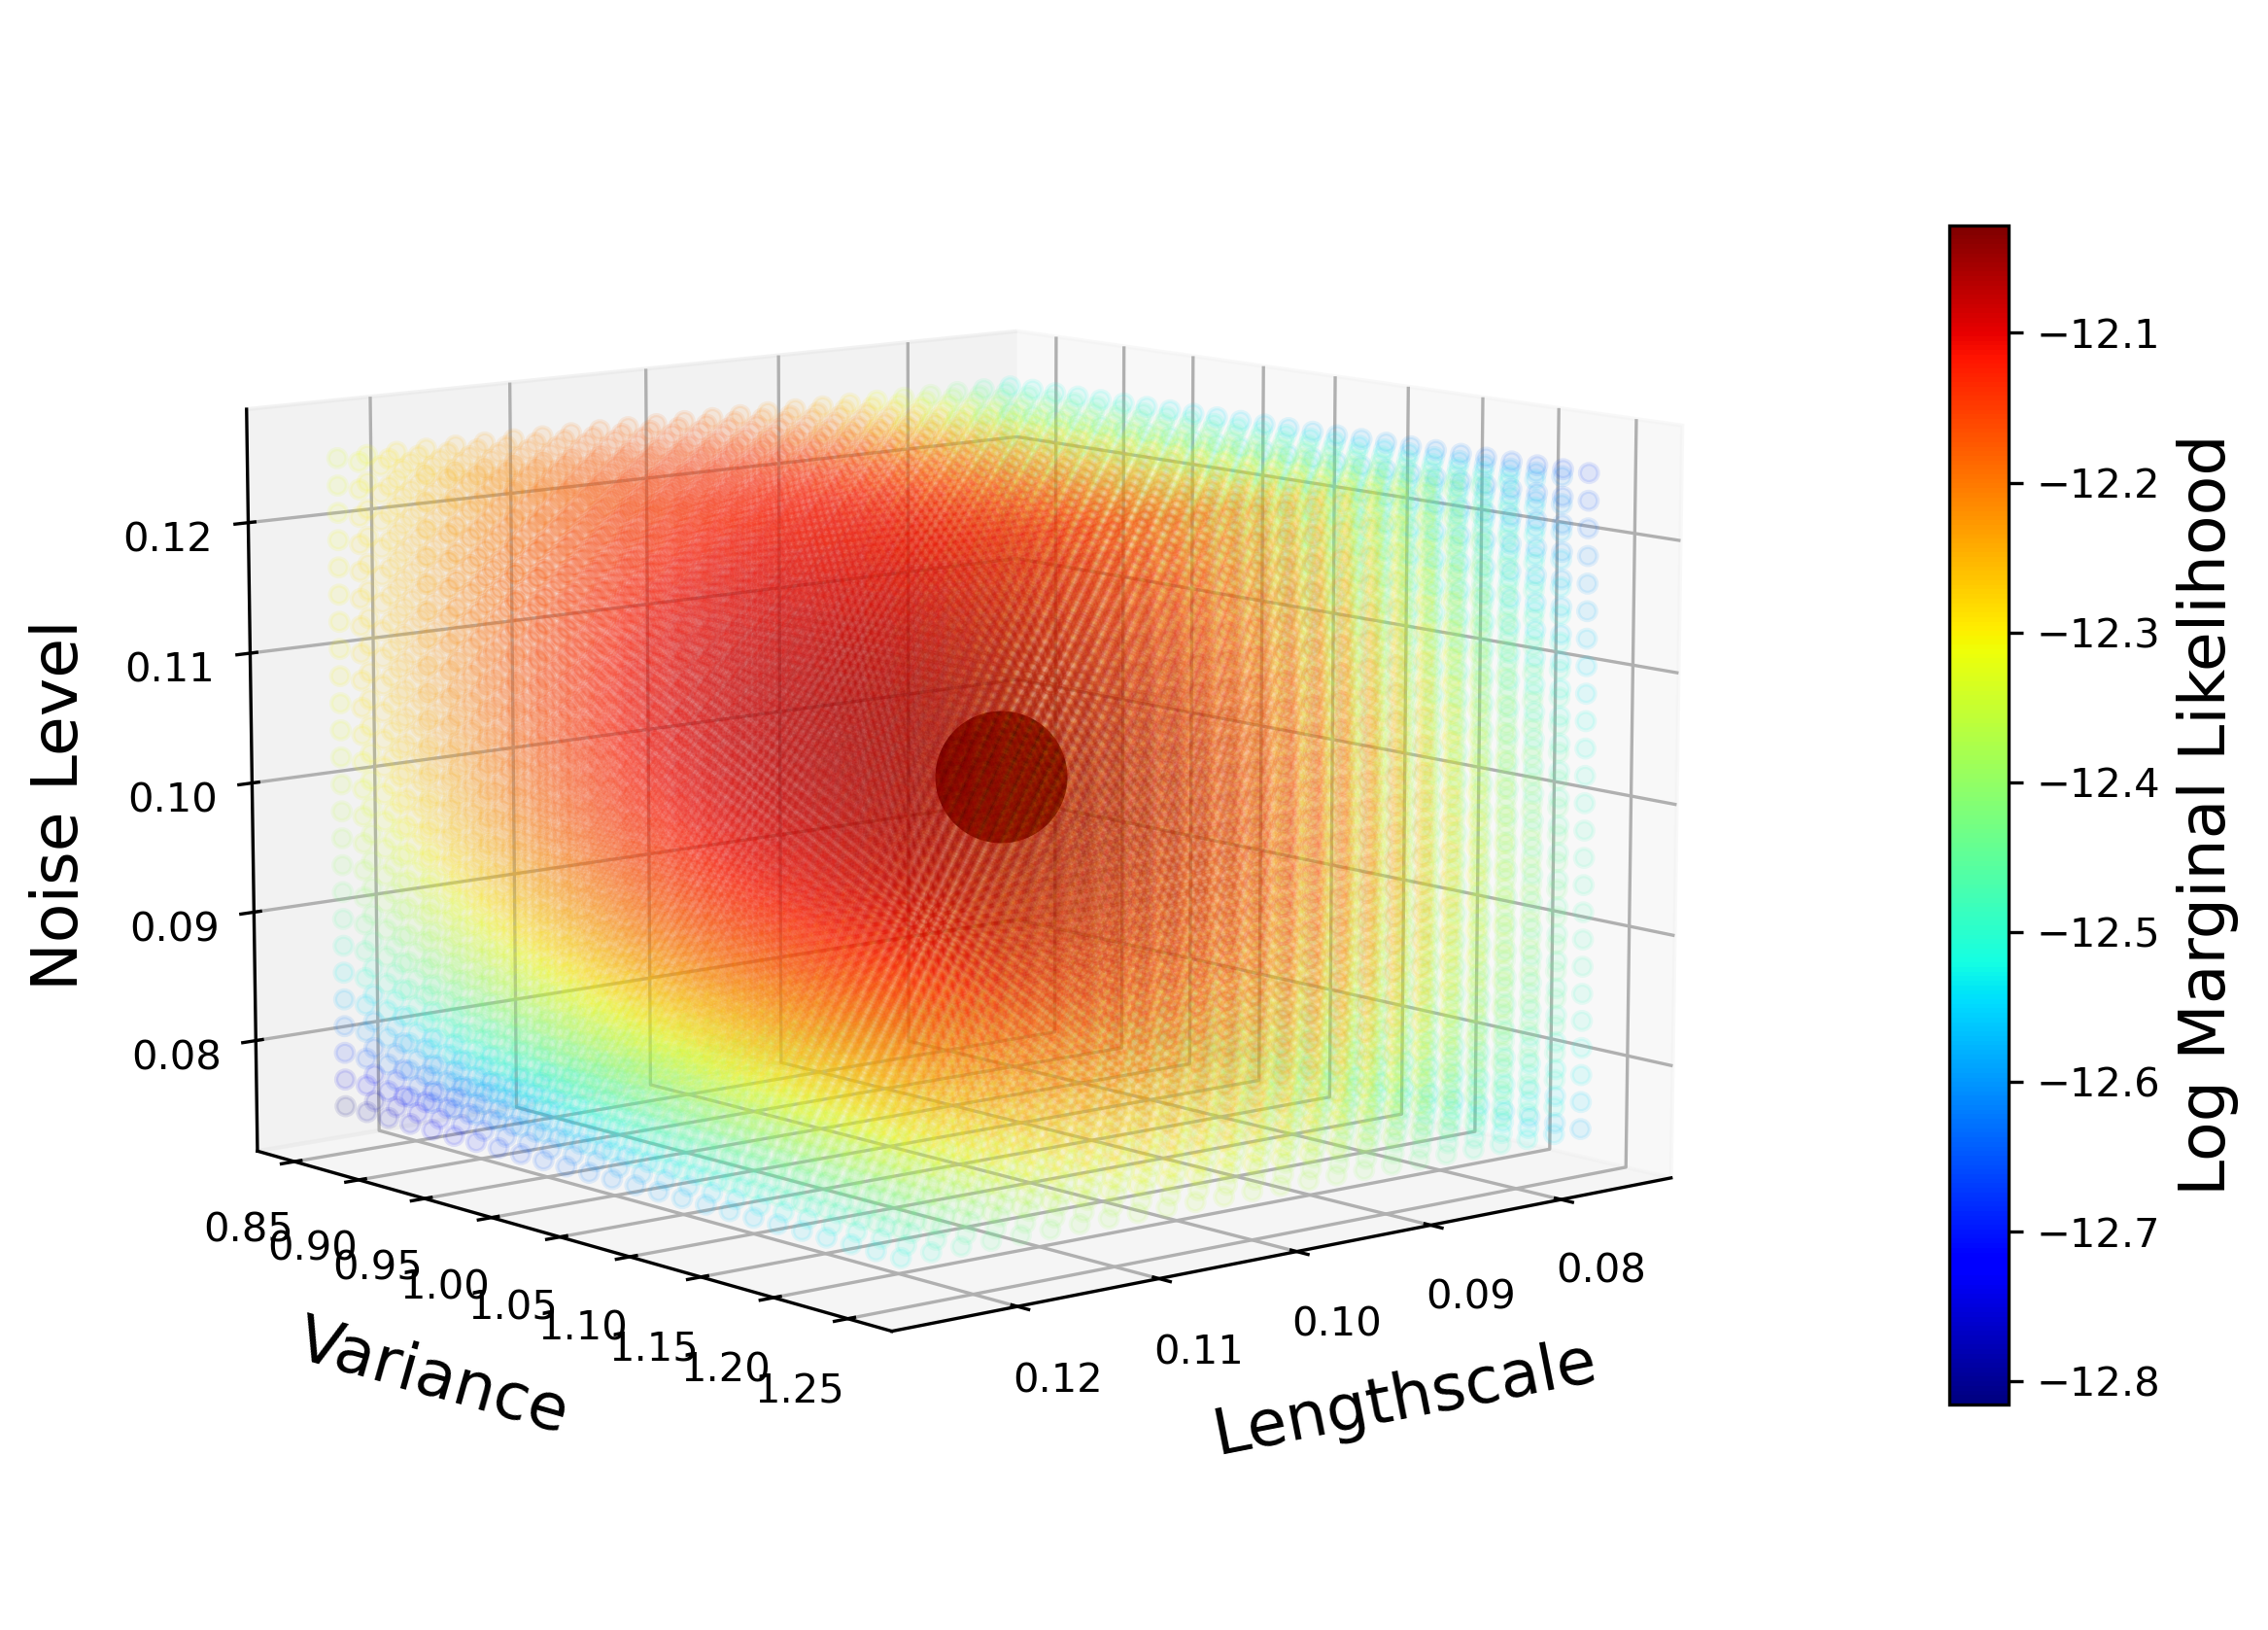
\includegraphics[width=\textwidth]{LatexPlots/1dplots/LogLike3params.png}
    \end{subfigure}
    \caption{For a GPR with noise we are forced to optimise a length hyper-parameter, a variance hyper-parameter and a noise hyper-parameter. 
    Here we have kept one parameter constant on each graph and compared the log likelihood space varying the other two parameters. 
    In graph one the noise is set at 0.1, in graph 2 the length is set at 0.5, in graph 3 the variance is set at 1.5. 
    In the final graph we plot a 3-dimensional scatter plot and illustrate the point estimate given by the optimisation algorithm as the black dot.This point is located at
    $(\sigma^2 = 1.16, l = 0.109$ noise$ = 0.105)$}
   \label{figure: Optimising Hyper-params}
\end{figure} 

\subsubsection{Cross Validation}


\subsection{Monte Carlo Markov Chain (MCMC): A Posterior over Hyperparameters}
\label{sec: MCMC}

\subsubsection{Why MCMC and the Mathematics Behind It}

We have discussed the role of kernels and how their hyperparameters affect the posterior distribution. From Figures~\ref{figure: Effect of Hyper-parameters} and~\ref{figure: Optimising Hyper-params}, we observed that when optimising hyperparameters, there is not necessarily a single "best" solution, but rather a region of valid values that explain the data well.

\noindent
Up to this point, the models we considered have relied on point estimates—selecting the hyperparameters that maximise the log marginal likelihood and using them for predictions. However, this approach ignores the uncertainty between hyperparameters that yield similarly high log-likelihood scores.
To address this uncertainty, we adopt a Bayesian perspective by using Markov Chain Monte Carlo (MCMC) methods to sample from the posterior distribution over hyperparameters. This approach allows us to move beyond point estimates and instead capture a full distribution that reflects uncertainty and variability in the hyperparameters.
By leveraging this posterior distribution, we gain a more comprehensive understanding of the model's behaviour. It allows for more robust predictions, better uncertainty quantification, and improved decision-making—especially in cases where multiple hyperparameter settings are plausible.

\bigskip
\noindent
When getting a point-estimate we maximised the log likelihood from equation \ref{eq: 5}. Now we want to build a distribution over the hyper-parameters. We have that:
\[
p(\theta \mid \mathbf{y}, X) = \frac{p(\mathbf{y} \mid X, \theta) \, p(\theta)}{p(\mathbf{y} \mid X)}
\]
where:
\begin{itemize}
    \item \( p(\mathbf{y} \mid X, \theta) \) is the likelihood,
    \item \( p(\theta) \) is the prior over hyperparameters,
    \item \( p(\mathbf{y} \mid X) \) is the marginal likelihood, acting as a normalising constant.
\end{itemize}

\noindent
Since \( p(\mathbf{y} \mid X) \) is often intractable, we sample from the unnormalised posterior using MCMC:
\[
p(\theta \mid \mathbf{y}, X) \propto p(\mathbf{y} \mid X, \theta) \, p(\theta)
\]

\noindent
Using MCMC, we generate samples \( \{\theta^{(s)}\}_{s=1}^S \sim p(\theta \mid \mathbf{y}, X) \) from this posterior.


\subsubsection{Implementing MCMC}
\begin{figure}[H]
    \centering
    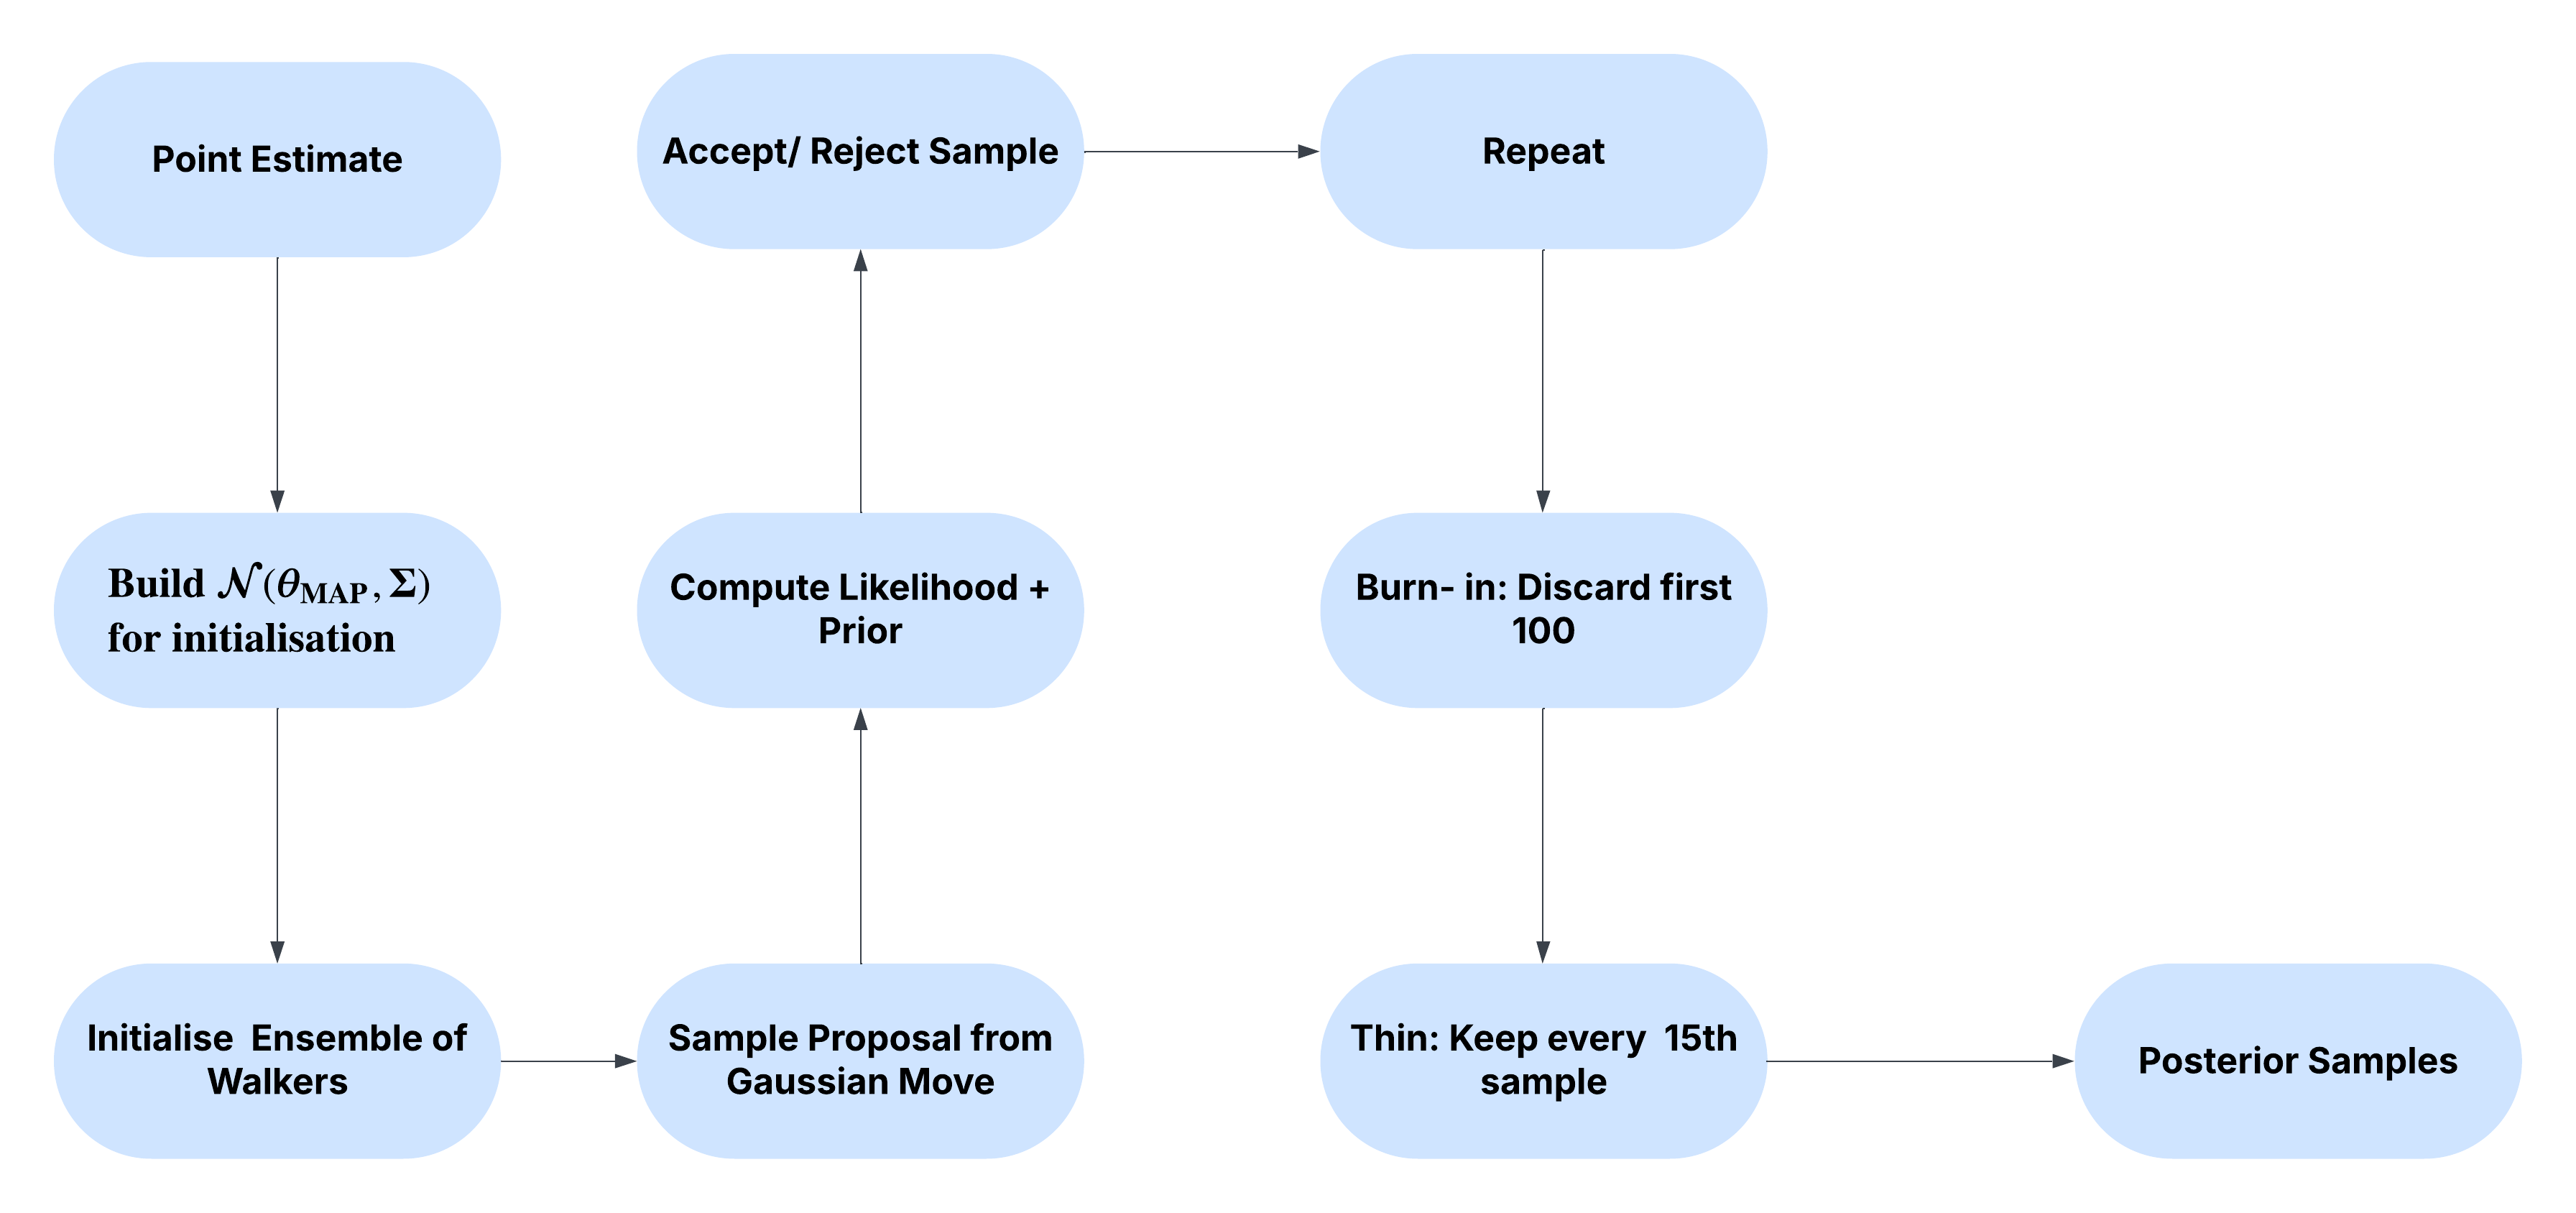
\includegraphics[width=0.8\textwidth]{LatexPlots/MCMC_Flow.png}
    \caption{Overview of the MCMC sampling procedure for Gaussian Process hyperparameter inference.
     This pipeline samples from the posterior \( p(\theta \mid \mathbf{y}, X) \) using a Metropolis-Hastings Gaussian proposal and an ensemble of walkers.}
    \label{fig:MCMC flowchart}
\end{figure}

\noindent
Before starting MCMC, we must decide which model we want to build the hyperparameter posterior for. This involves selecting one of the six kernels outlined in Section~\ref{sec: Kernels}, along with one of the three noise-modelling approaches described in Section~\ref{sec: Handlingnoise}. Once this model structure is fixed, we obtain initial point estimates for the hyperparameters by maximising the log marginal likelihood, as discussed in Section~\ref{sec: hyperparam optimisation}.

\noindent
We then construct a multivariate normal distribution centred at this point estimate and sample from it to initialise each walker. From there, the walkers explore the hyperparameter space using a Gaussian proposal distribution with a specified covariance. At each step, we compute the sum of the log likelihood and log prior. The proposed sample is then accepted or rejected using the Metropolis-Hastings criterion \textcolor{red}{Could give more detail here}. This process is repeated for a fixed number of steps to generate a large set of samples.

\noindent
To ensure convergence and sample independence, we discard the first 100 samples from each walker as burn-in and apply a thinning factor of 15—retaining every 15\textsuperscript{th} sample. The resulting collection of samples forms our posterior distribution over hyperparameters, which we visualise using a kernel density estimate (KDE).


\begin{figure}[H]
    \centering
    \begin{subfigure}[b]{0.48\textwidth}
        \centering
        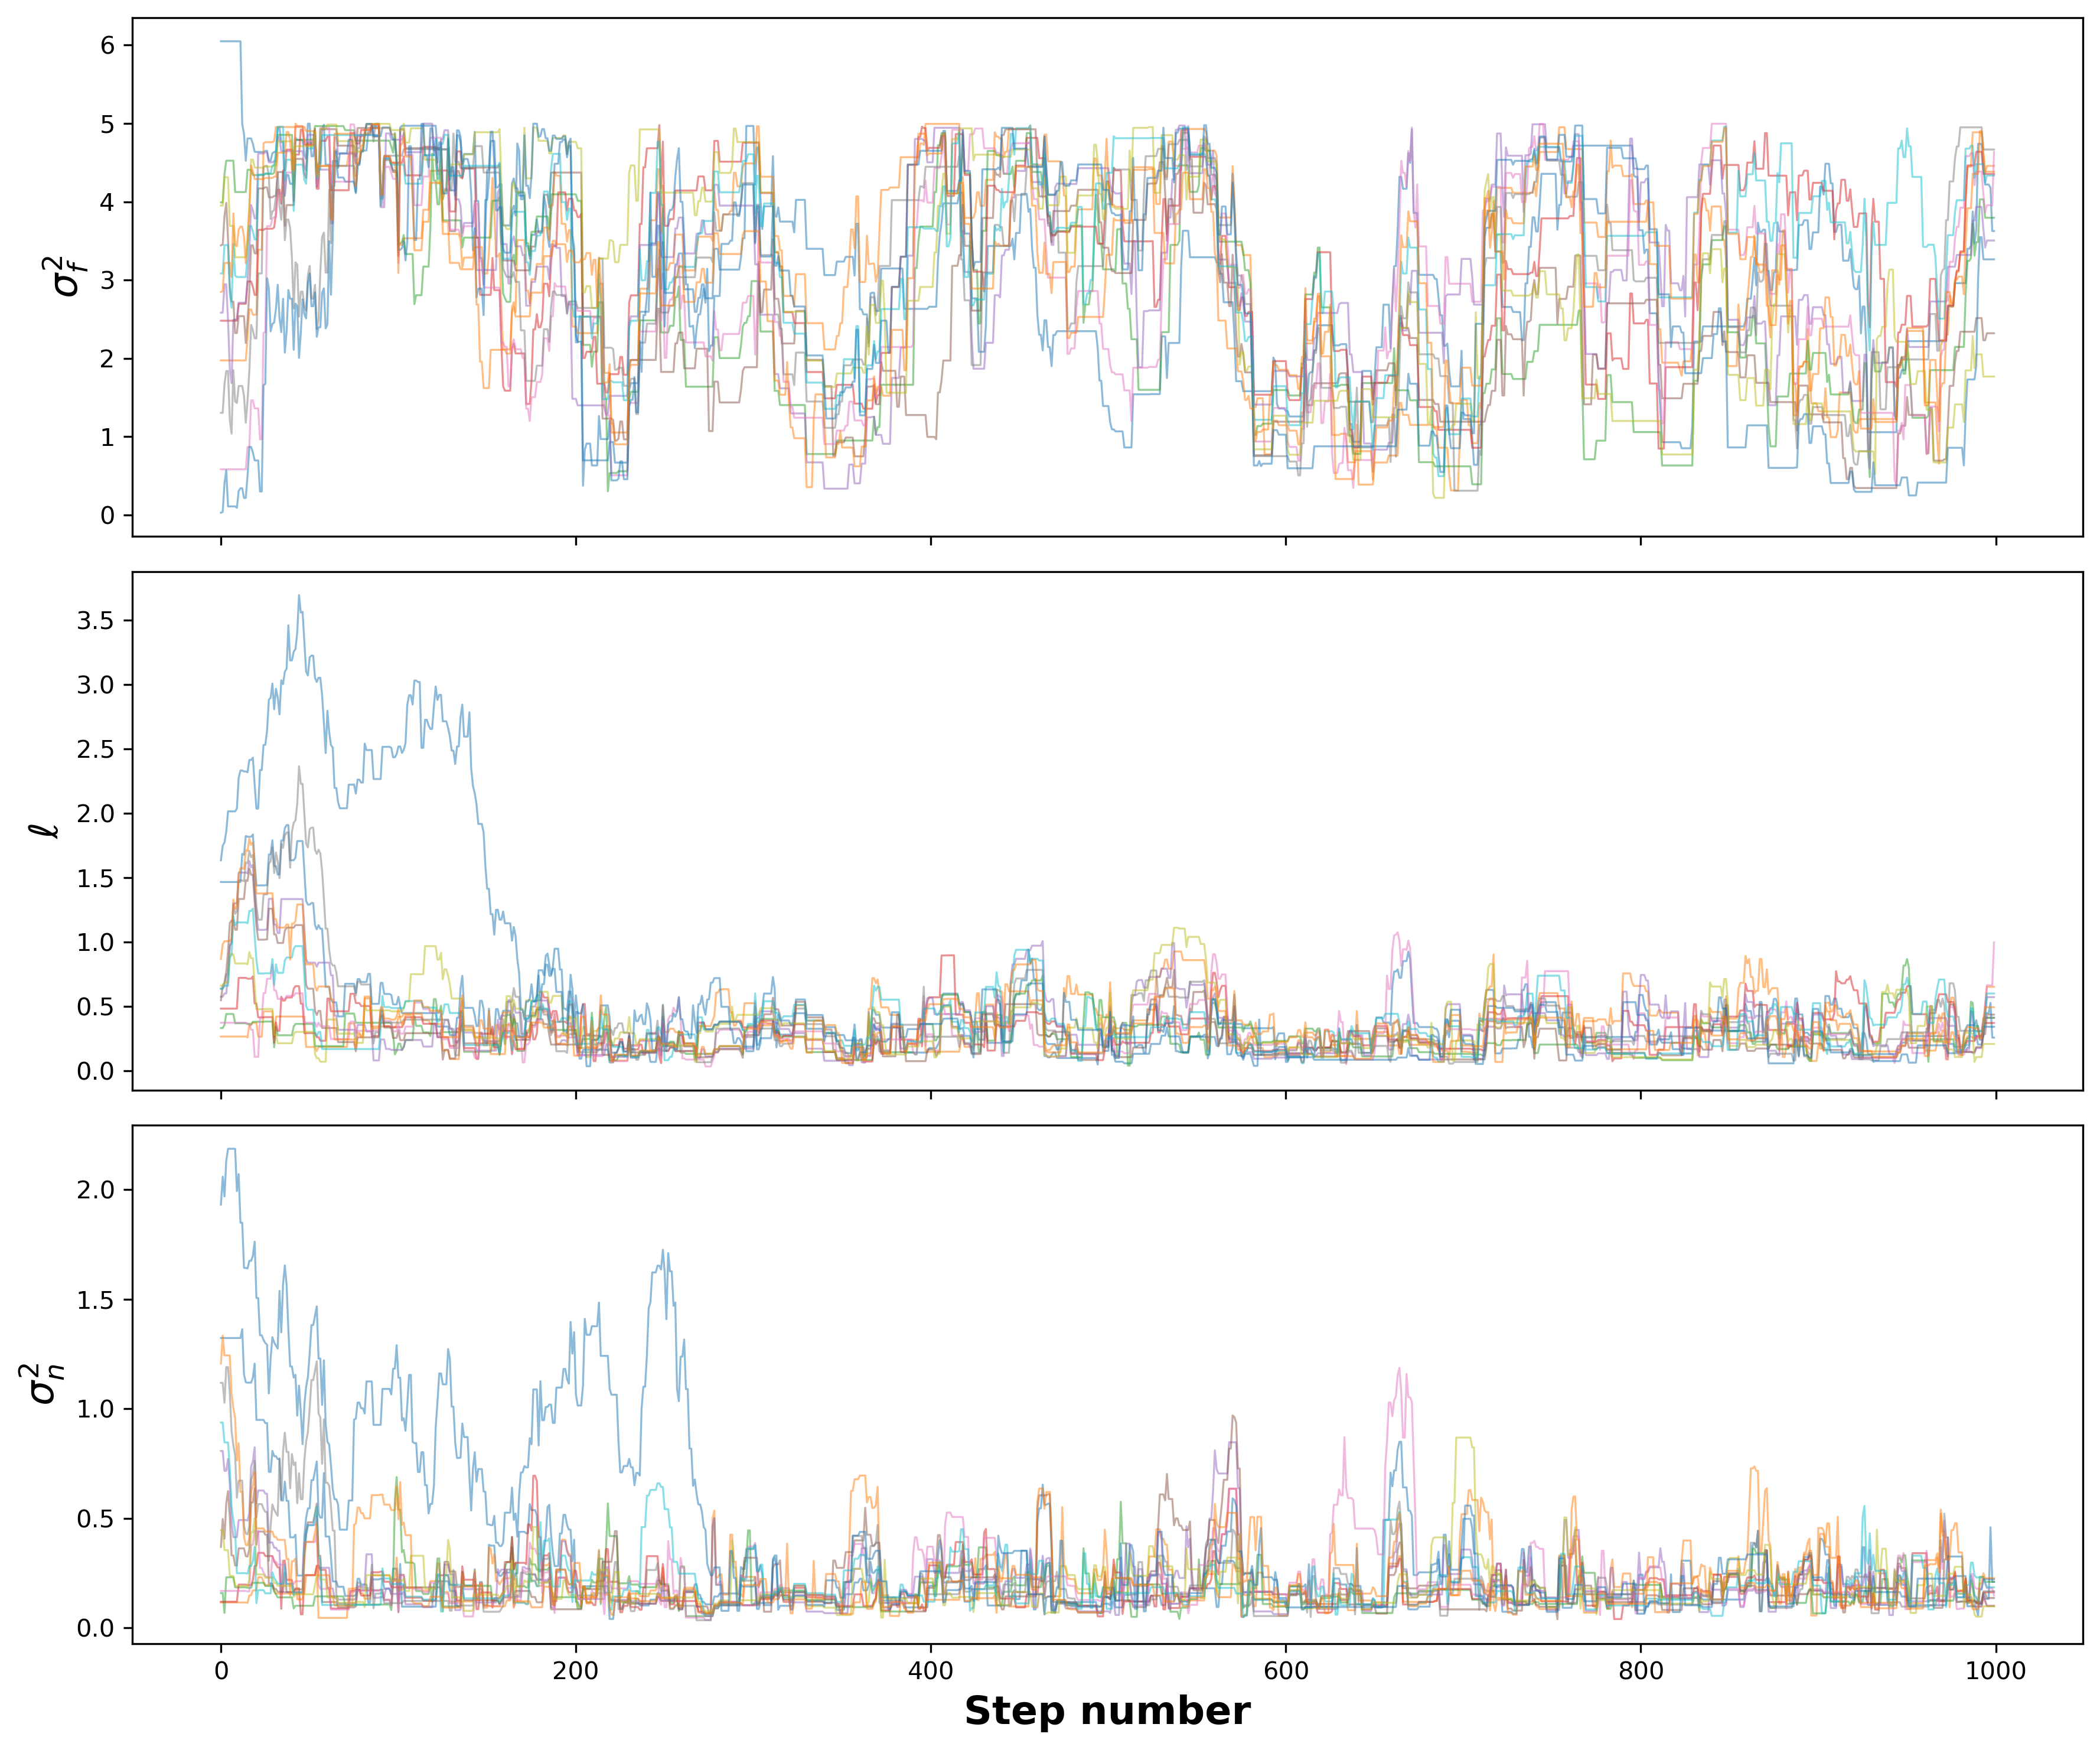
\includegraphics[width=\textwidth]{LatexPlots/1dplots/MCMCwalkers.png}
    \end{subfigure}
    \hfill
    \begin{subfigure}[b]{0.48\textwidth}
        \centering
        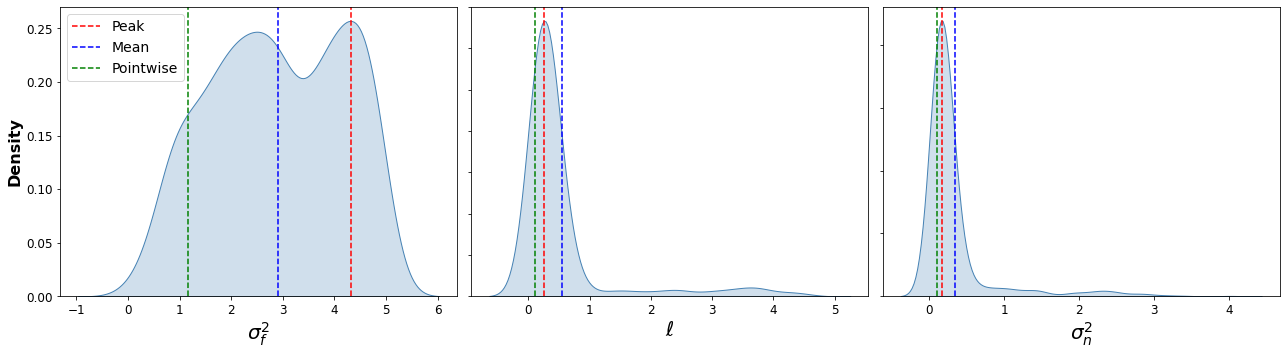
\includegraphics[width=\textwidth]{LatexPlots/1dplots/MCMCdistribution.png}
    \end{subfigure}
    \caption{This MCMC is run using a gpr with a RBF Kernel with White Kernel for noise.Left: A plot of the space sampled by each walker in my MCMC run (burnin=100 and thin=15). \quad Right: A plot of the distribution of the hyper-parameters built using a Gaussian KDE from the MCMC samples.}
    \label{fig:MCMCresults}
\end{figure}
\noindent
We can see from the distributions in \ref{fig:MCMCresults} that the variance hyper-paramterer is almost bi-modal (i.e has two significant peaks). For our bi-model hyper-parameter we can see that the mean parameter, peak parameter and point estimate parameter differ significantly.
In this scenario any singular point estimate will lose a lot of information about the distribution particularly for the variance hyper-parameter. To resolve this we can instead of picking a singular point build
the hyper-parameter uncertainty into our final predictive distribution.


\noindent
We previously had our predictive distribution as :
\[
p(f_* \mid \mathbf{y}, X, X_*, \theta),
\]
where predictions were made conditional on a fixed set of hyperparameters \( \theta \). Now, we marginalise over the posterior distribution of \( \theta \) to account for hyperparameter uncertainty:
\[
p(f_* \mid \mathbf{y}, X, X_*) = \int p(f_* \mid \mathbf{y}, X, X_*, \theta) \, p(\theta \mid \mathbf{y}, X) \, d\theta.
\]

\noindent
Since this integral is analytically intractable, we approximate it using the MCMC samples \( \{\theta^{(s)}\}_{s=1}^S \):
\[
p(f_* \mid \mathbf{y}, X, X_*) \approx \frac{1}{S} \sum_{s=1}^{S} p(f_* \mid \mathbf{y}, X, X_*, \theta^{(s)}).
\]

\noindent
This entails constructing a full posterior predictive distribution for each set of sampled hyperparameters and then averaging across all predictions. In practice, we compute the final predictive mean and variance using the law of total variance:
\[
\mathbf{E}[f_*] \approx \frac{1}{S} \sum_{s=1}^{S} \mu^{(s)}(f_*),
\]
\[
\text{Var}[f_*] \approx \frac{1}{S} \sum_{s=1}^{S} \left[ \sigma^{2(s)}(f_*) + \left(\mu^{(s)}(f_*)\right)^2 \right] - \left( \mathbf{E}[f_*] \right)^2,
\]
where \( \mu^{(s)}(f_*) \) and \( \sigma^{2(s)}(f_*) \) are the predictive mean and variance obtained from the \( s \)-th sampled hyperparameter configuration \( \theta^{(s)} \).


\noindent
This procedure yields a predictive distribution that fully reflects both the uncertainty in the data and the uncertainty in the model's hyperparameters



\begin{figure}[H]
    \centering
    \begin{subfigure}[b]{0.3\textwidth}
        \centering
        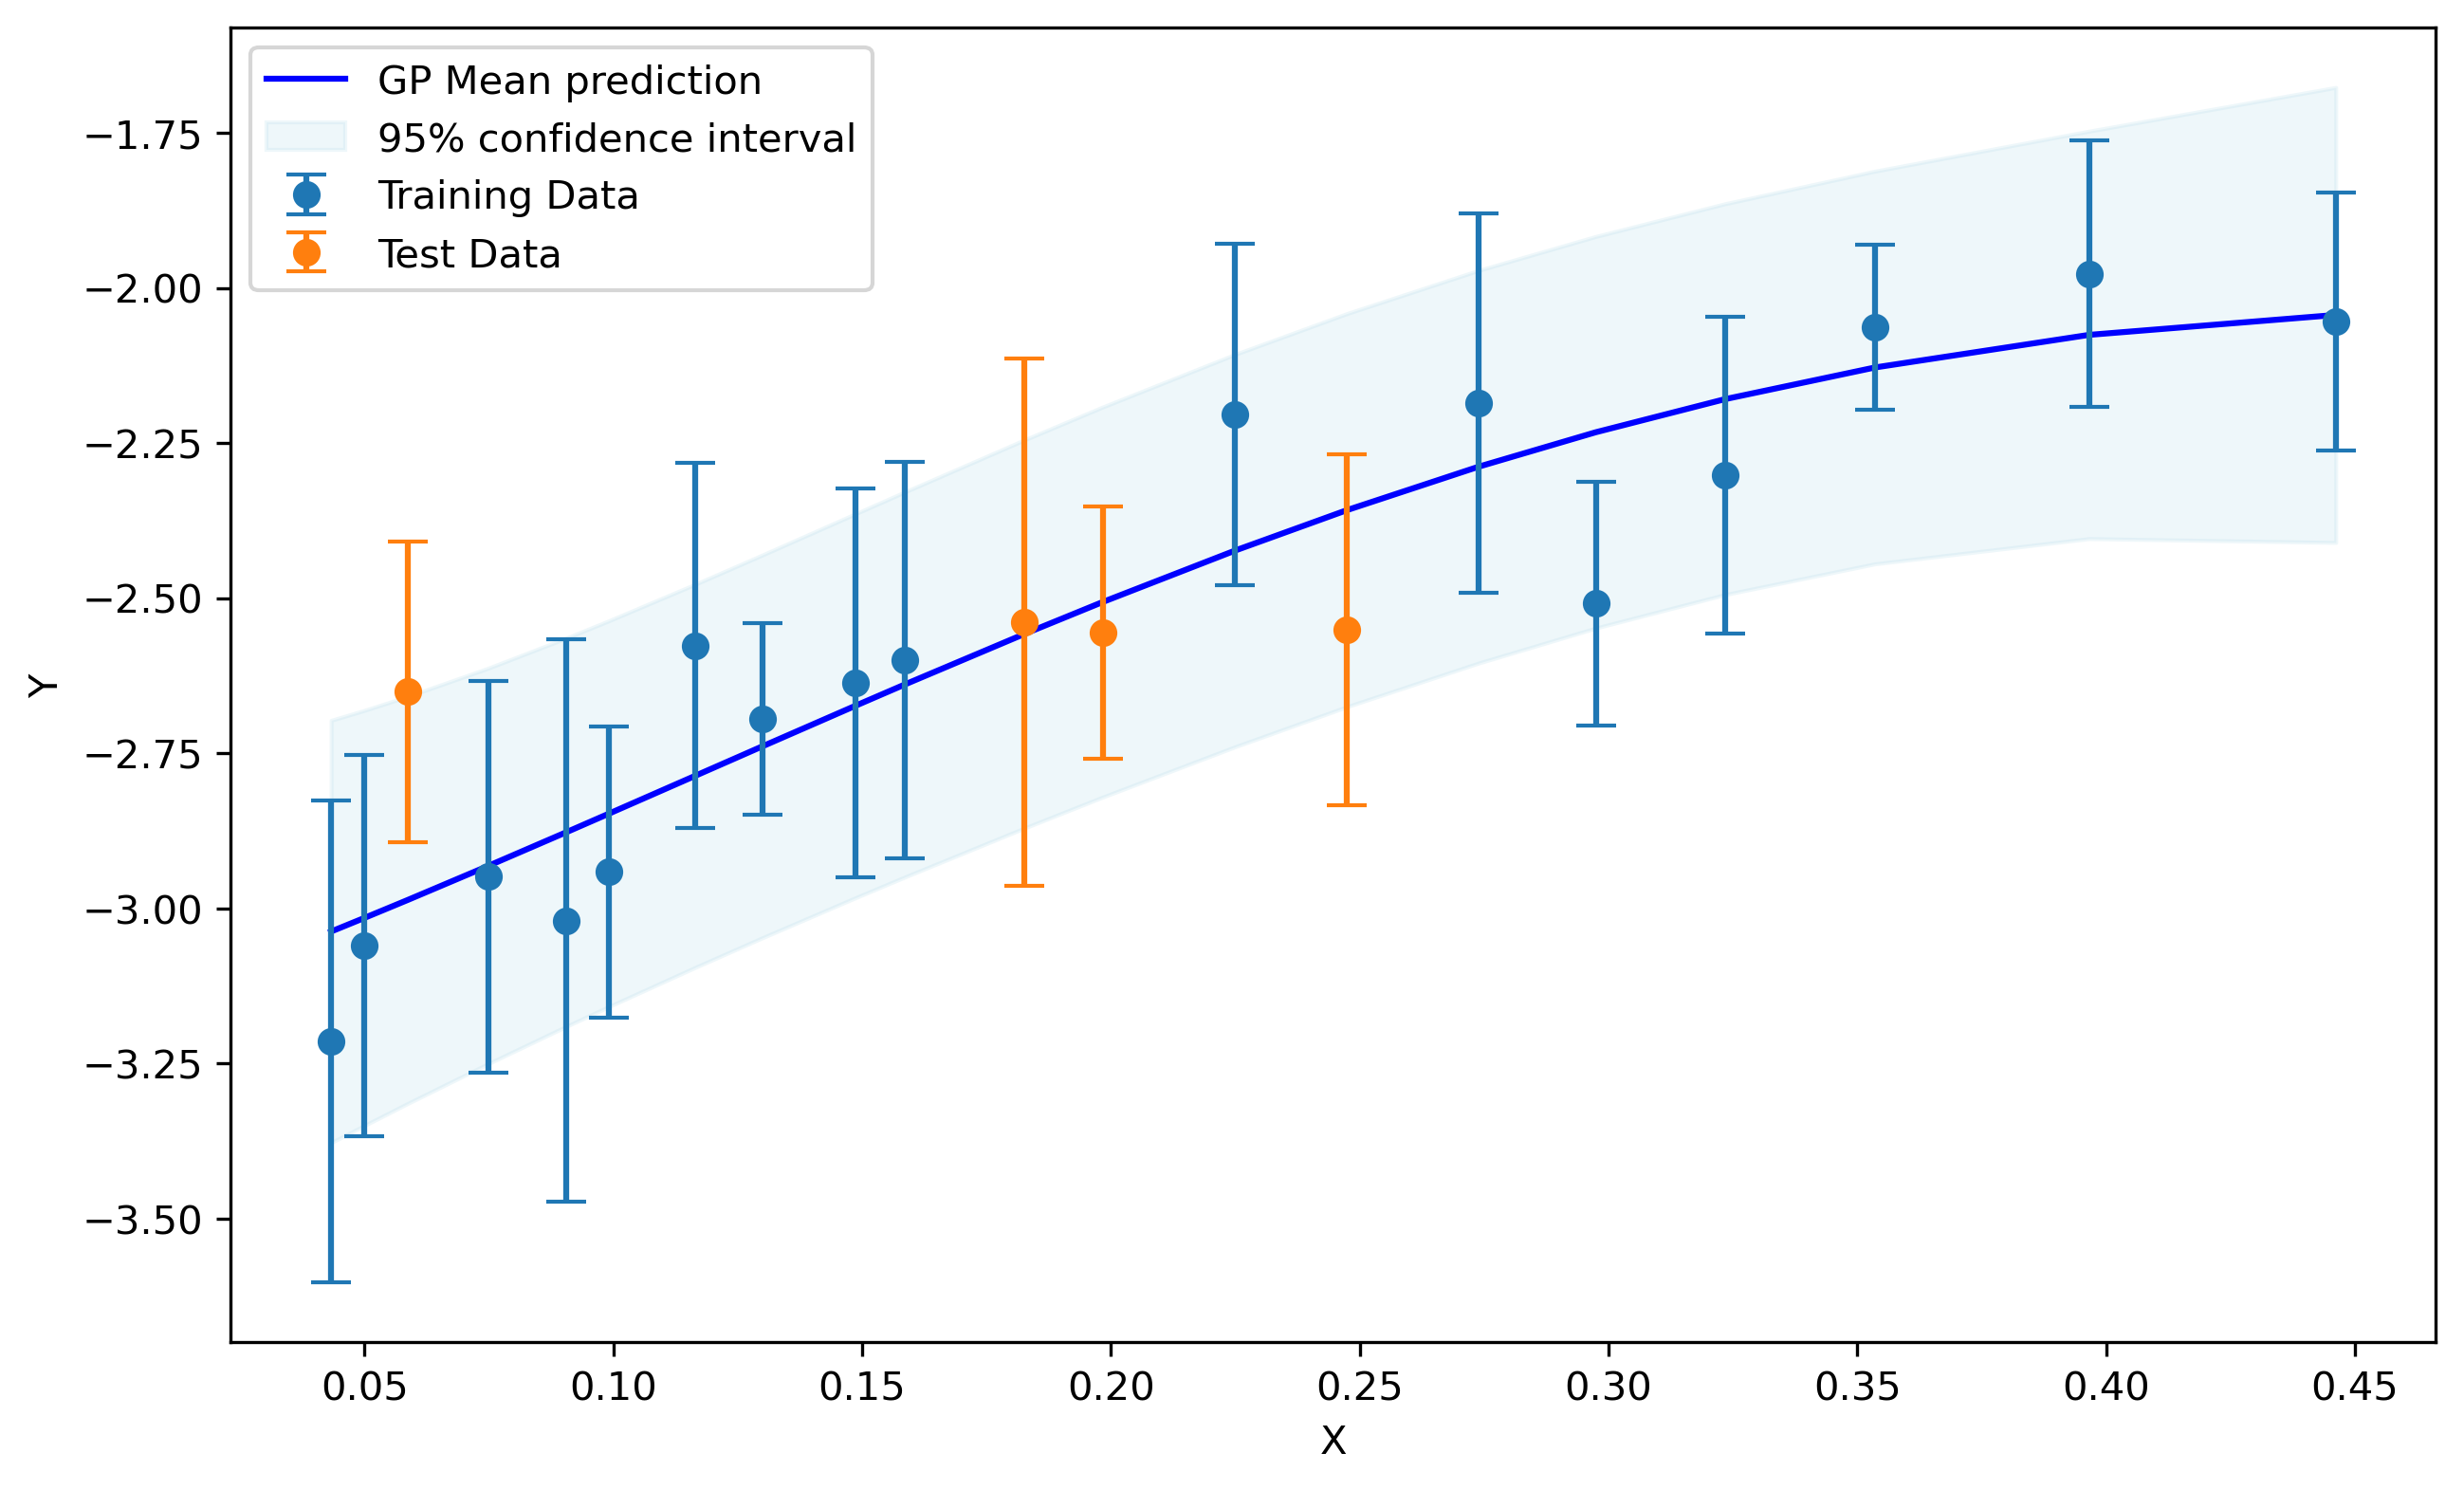
\includegraphics[width=\textwidth]{LatexPlots/1dplots/MCMCmeangpr.png}
    \end{subfigure}
    \hfill
    \begin{subfigure}[b]{0.3\textwidth}
        \centering
        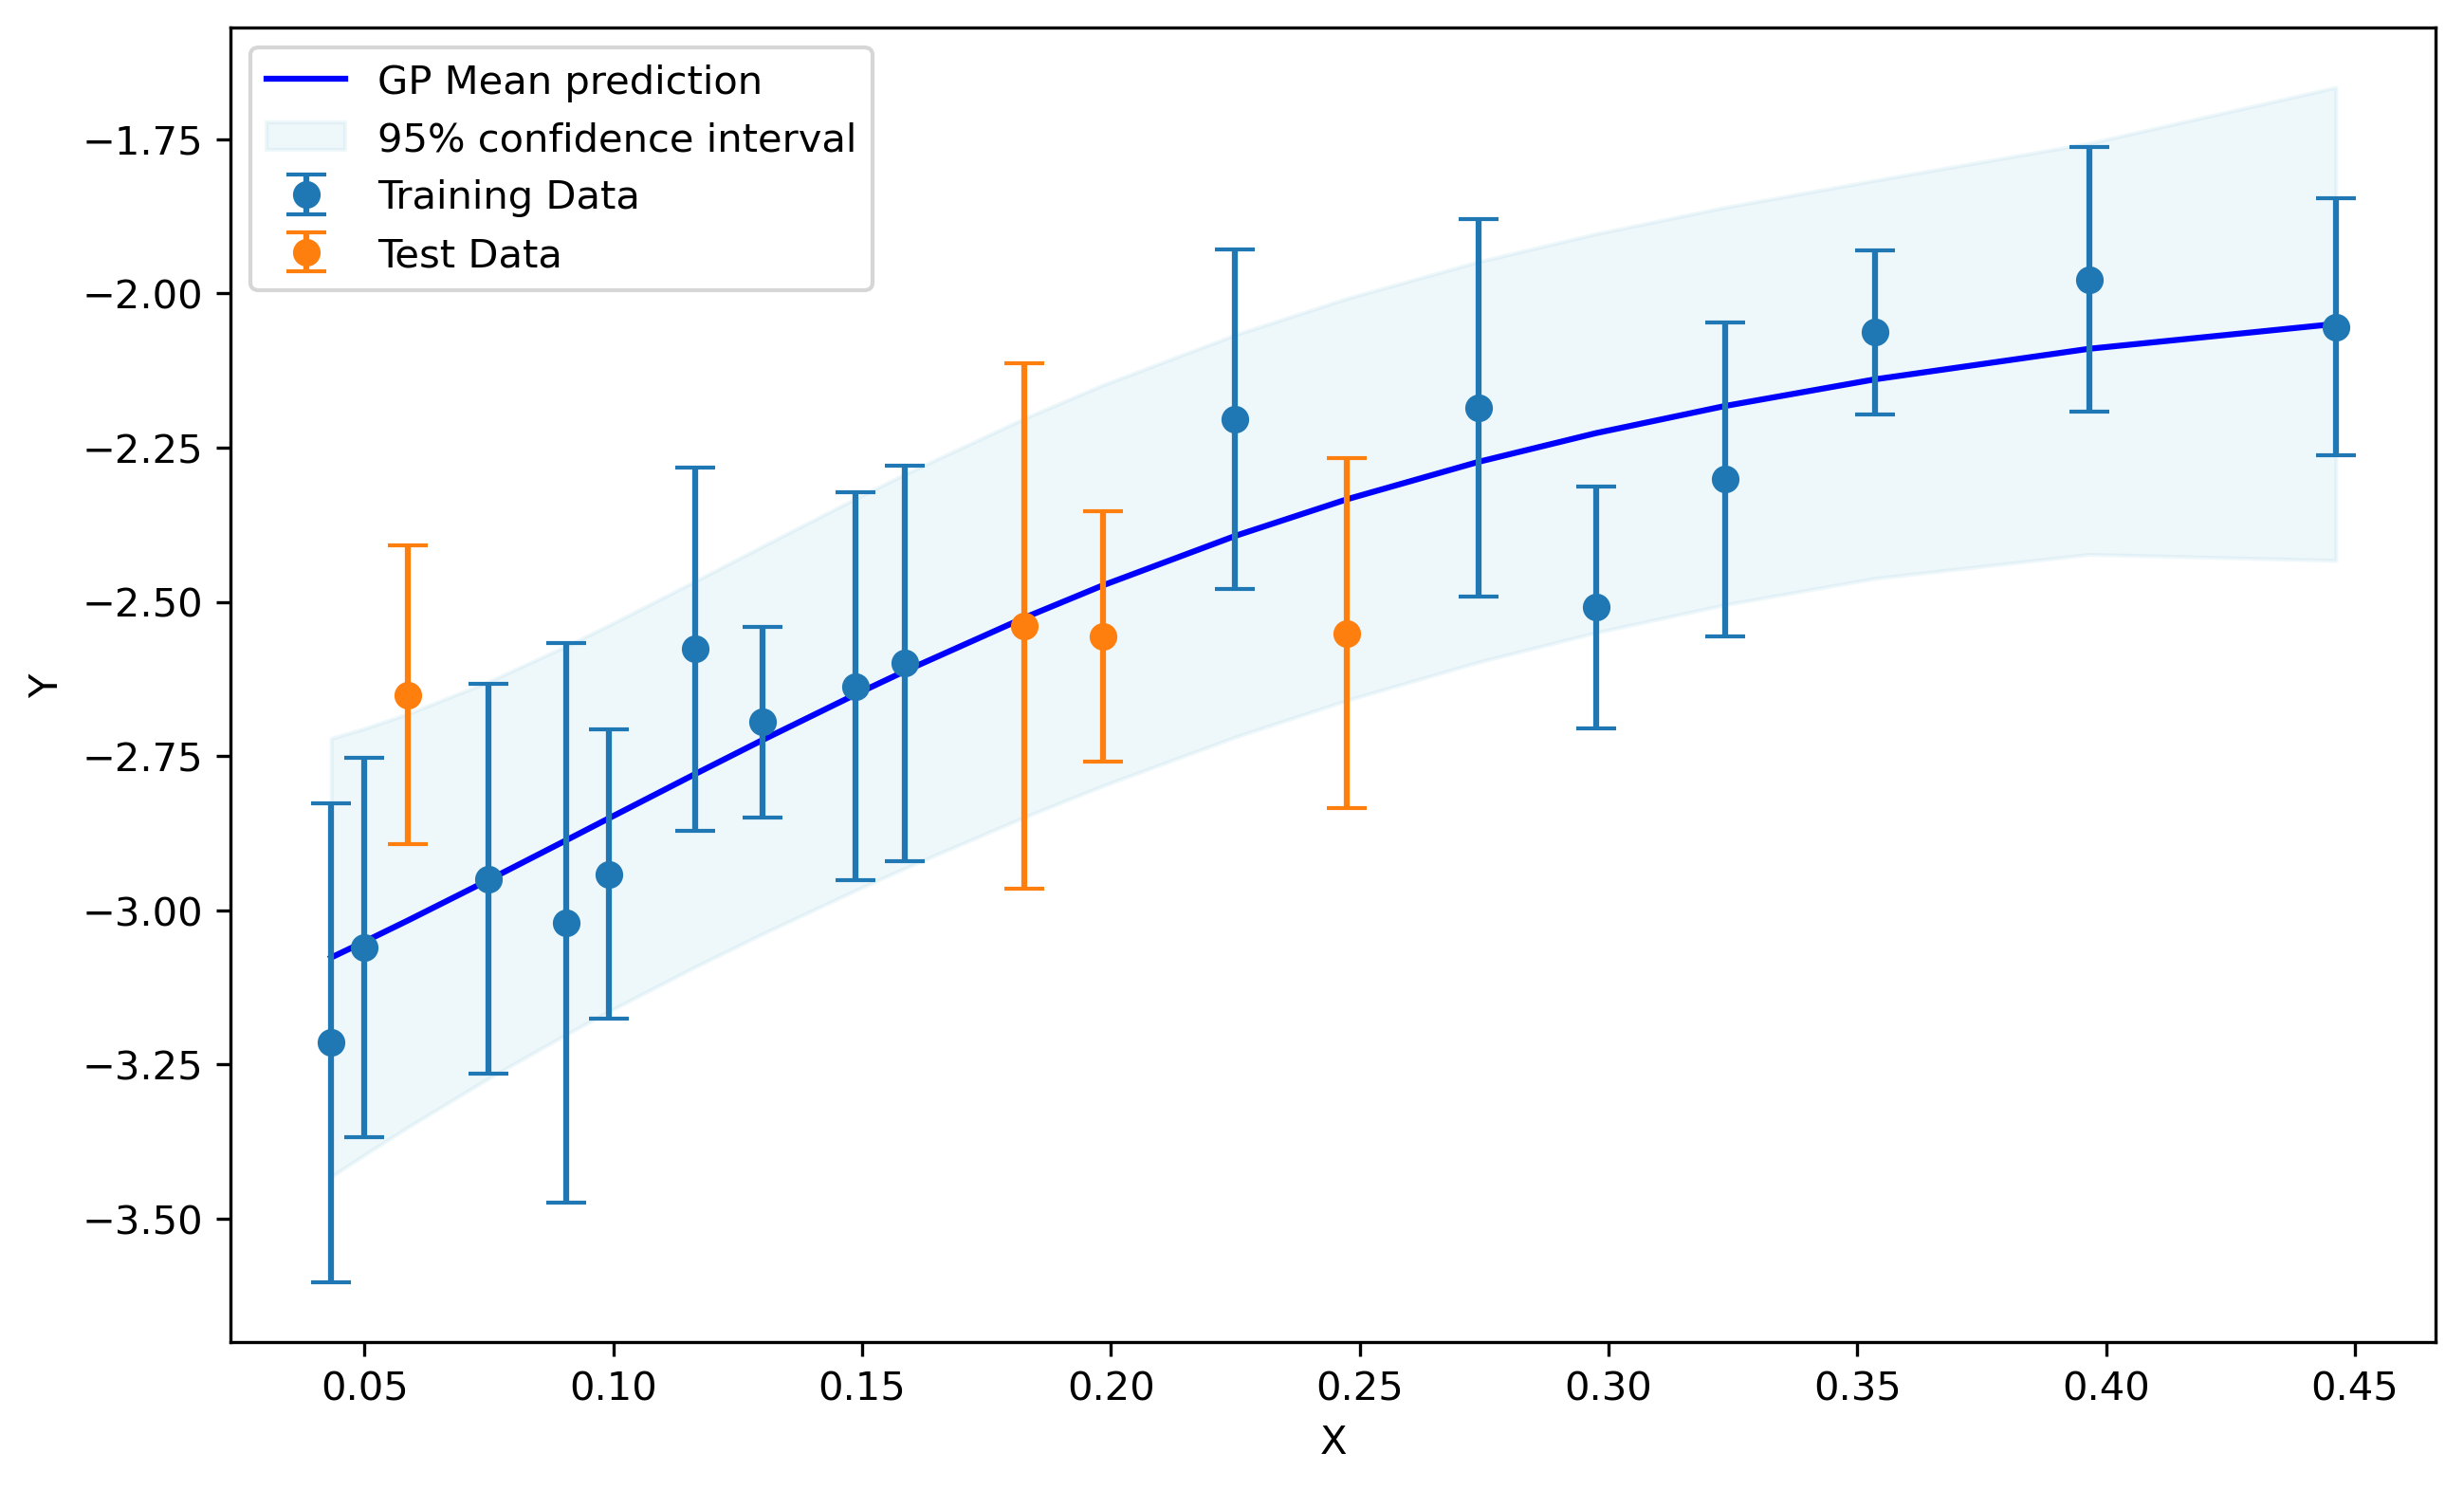
\includegraphics[width=\textwidth]{LatexPlots/1dplots/MCMCpeakgpr.png}
    \end{subfigure}
    \hfill
    \begin{subfigure}[b]{0.3\textwidth}
        \centering
        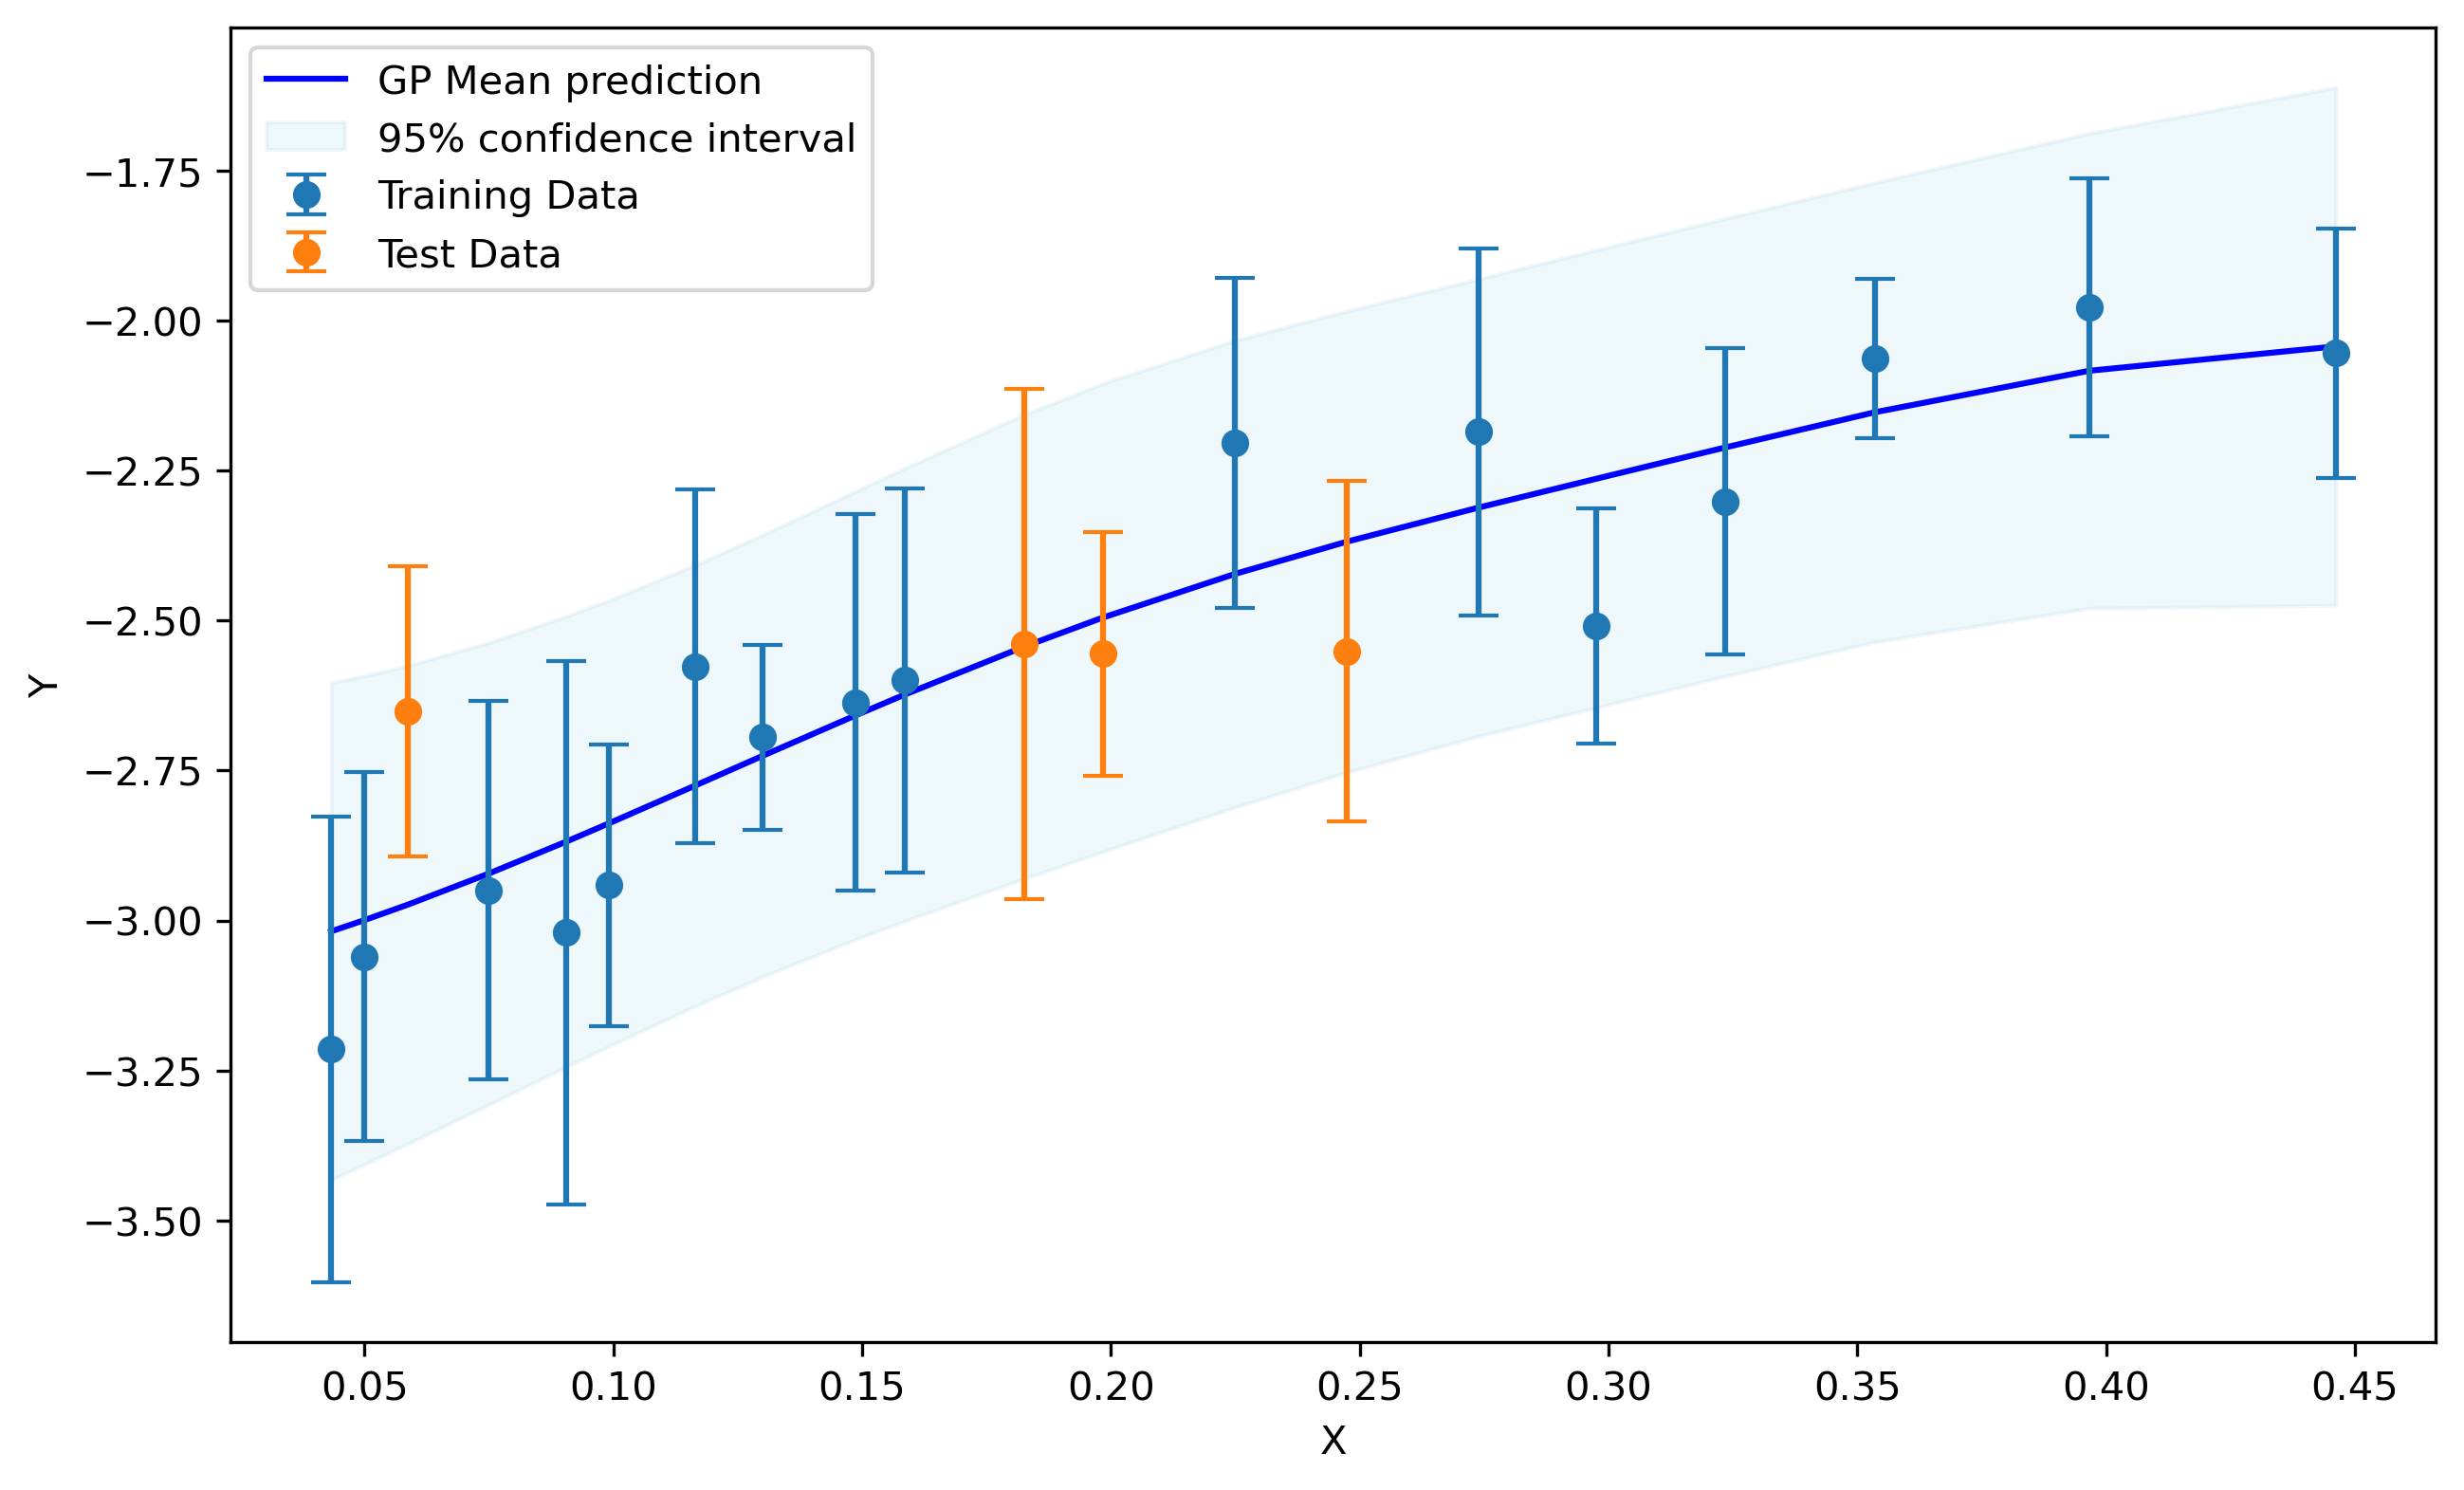
\includegraphics[width=\textwidth]{LatexPlots/1dplots/MCMCaveragegpr.png}
    \end{subfigure}
    \caption{
        Left: This is the GPR plotted with the mean hyper-parameters
        Middle: This is the GPR plotted with the peak hyper-parameters
        Right: This is the full predictive distribution over all the hyper-parameter samples
     }
\end{figure}



\subsection{Metrics for testing model}


In figure \ref{tab:metrics-comparison}, we made a graphical representation of four out of six metrics used to evaluate our model’s accuracy. \cite{rasmussen2006gaussian} discusses how these metrics provide a balanced assessment of model performance.
The Root Mean Squared Error (RMSE) and Mean Absolute Error (MAE) measure the average deviation of predictions from the true values, with RMSE penalizing larger errors more heavily.
The coefficient of determination \( R^2 \) quantifies how well the model predicts relative to the mean of the test set. It is computed as \( 1 \) minus the ratio of the squared residuals to the total variance. A value closer to \( 1 \) indicates better predictive performance.
The adjusted \( R^2 \) (\(\bar{R}^2\)) accounts for model complexity by penalizing excessive predictor variables, preventing overfitting.
The Figure of Merit (FOM) evaluates the ratio of a point’s prediction error to its associated standard deviation. A FOM near \( 1 \) is ideal, indicating that the model’s uncertainty estimates are well-calibrated. A FOM \( \ll 1 \) suggests an overly conservative model with large uncertainty, while a FOM \( \gg 1 \) may indicate overconfidence, failing to capture true variability.
The Pearson correlation coefficient measures the linear relationship between predictions and true values. A correlation of \( 1 \) (\(-1\)) signifies a perfect positive (negative) linear relationship, whereas a correlation of \( 0 \) indicates no linear association.



\begin{table}[H]
    \centering
    \renewcommand{\arraystretch}{4} % Adjust row spacing
    \setlength{\tabcolsep}{2pt} % Adjust column spacing
    \small % Reduce text size

    \begin{tabular}{|>{\centering\arraybackslash}m{2.5cm}|*{4}{>{\centering\arraybackslash}m{3cm}|}} 
        \hline
        \textbf{Metric Name} & \textbf{RMSE} & \textbf{\(R^2\)} & \textbf{FOM} & \textbf{Pearson Coefficient} \\ 
        \hline
        \textbf{Formula} & 
        \( \sqrt{\frac{1}{N} \sum (y_i - \hat{y}_i)^2} \)   & 
        \( 1 - \frac{\sum (y_i - \hat{y}_i)^2}{\sum (y_i - \bar{y})^2} \) &    
        \( \frac{RMSE}{\sigma} \) &  
        \( \frac{\text{cov}(y - \hat{y})}{\sigma_y \sigma_{\hat{y}}} \) \\ 
        \hline
        \textbf{Visual Illustration} &  
        \adjustbox{valign=c}{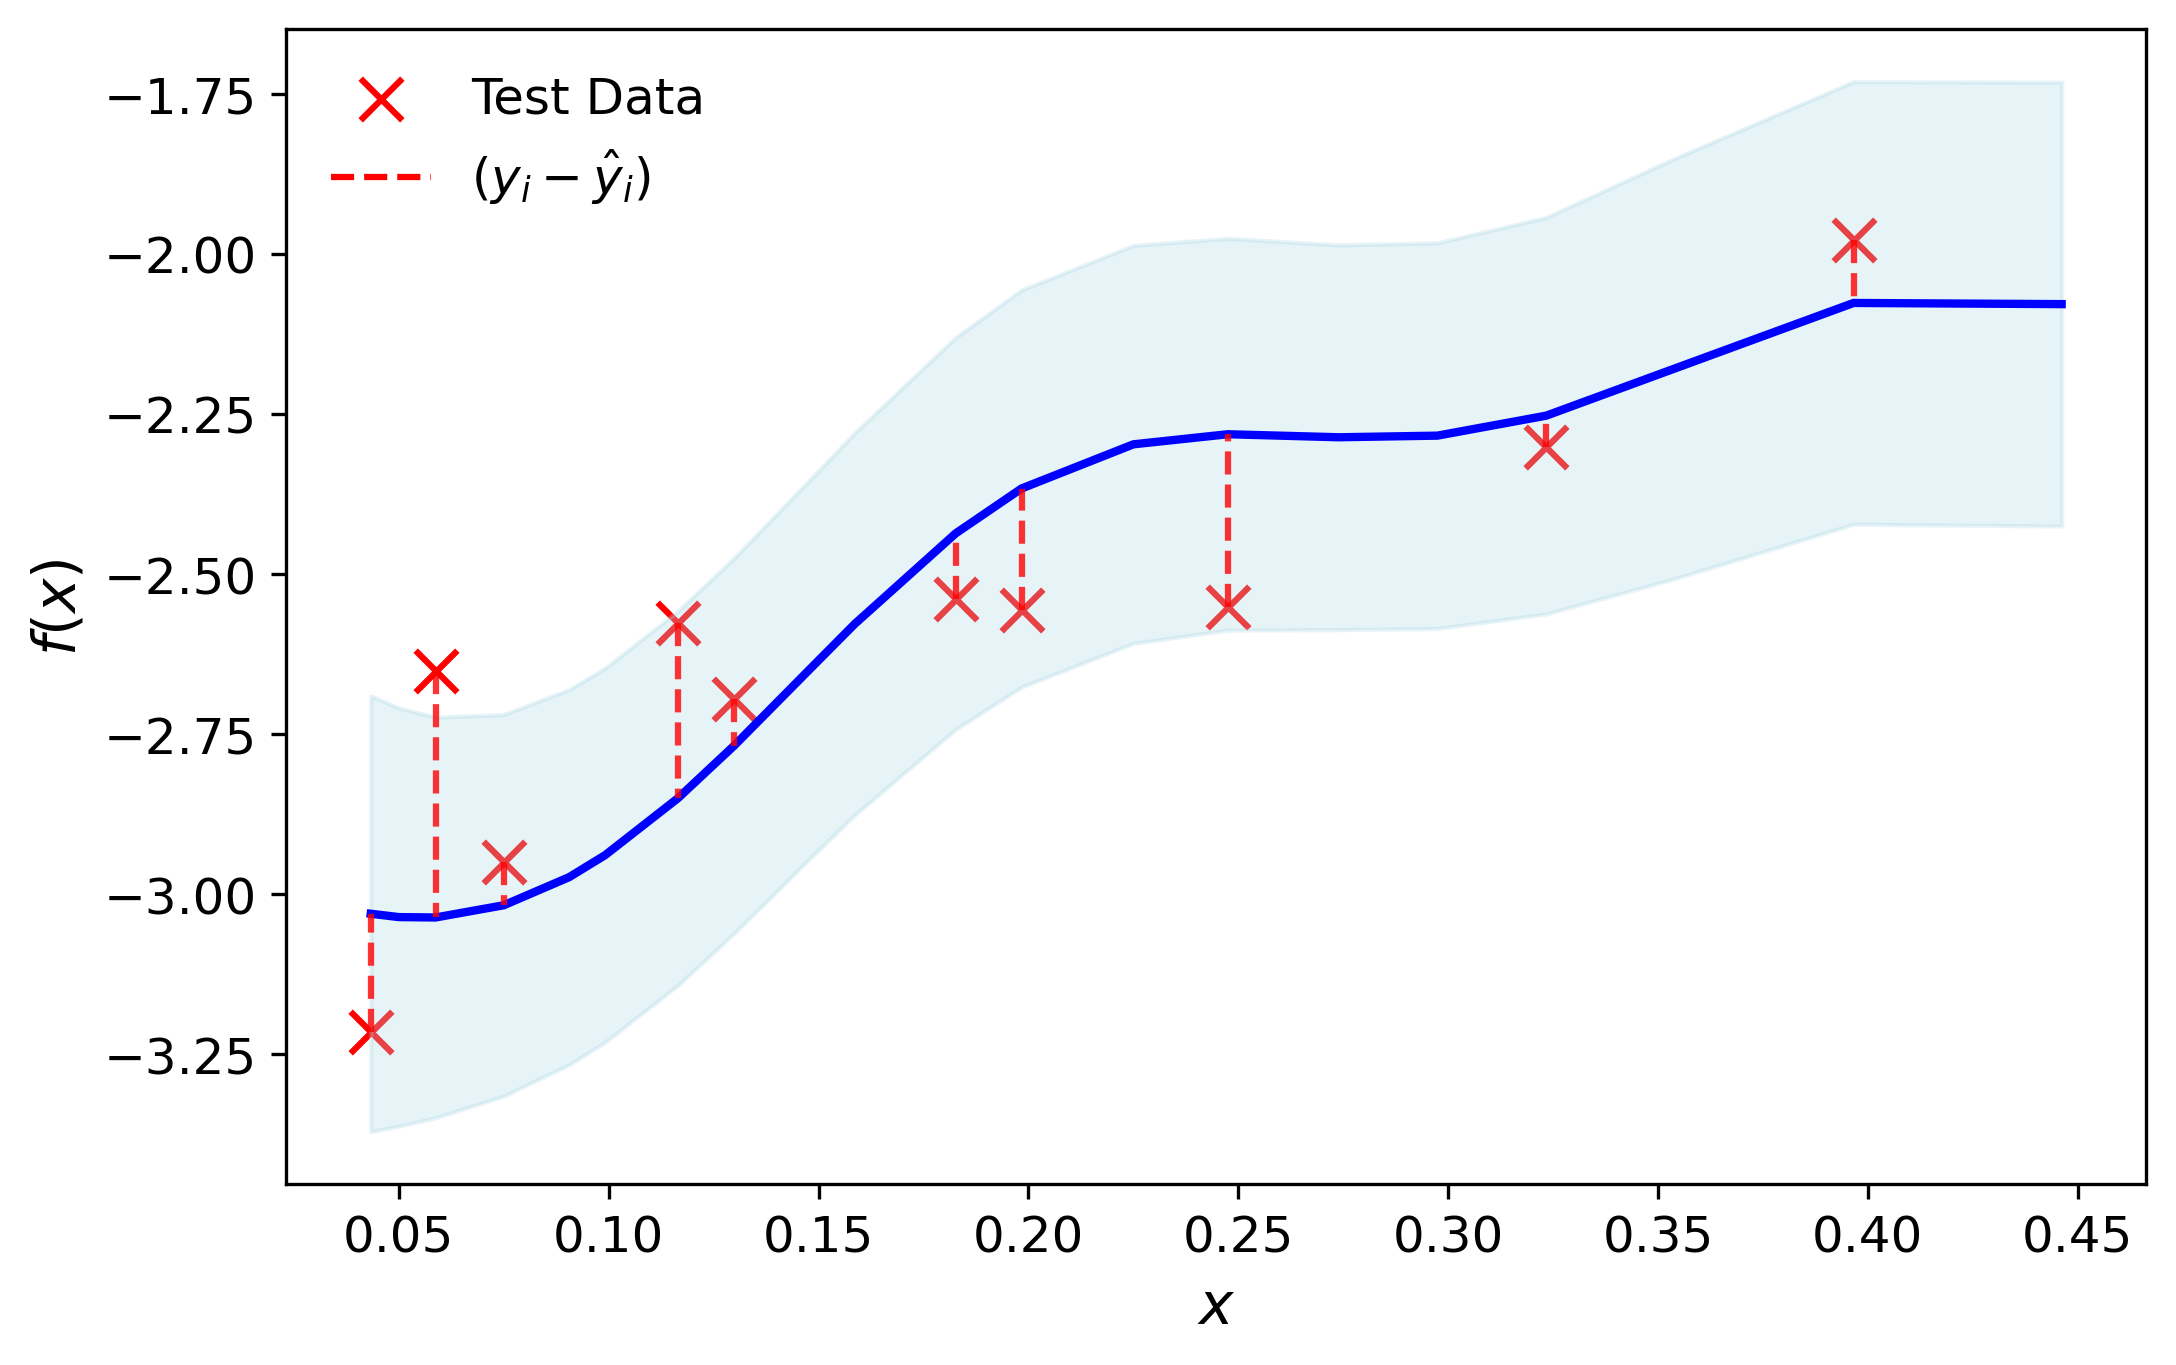
\includegraphics[width=3cm]{LatexPlots/1dplots/MAE.png}} &  
        \adjustbox{valign=c}{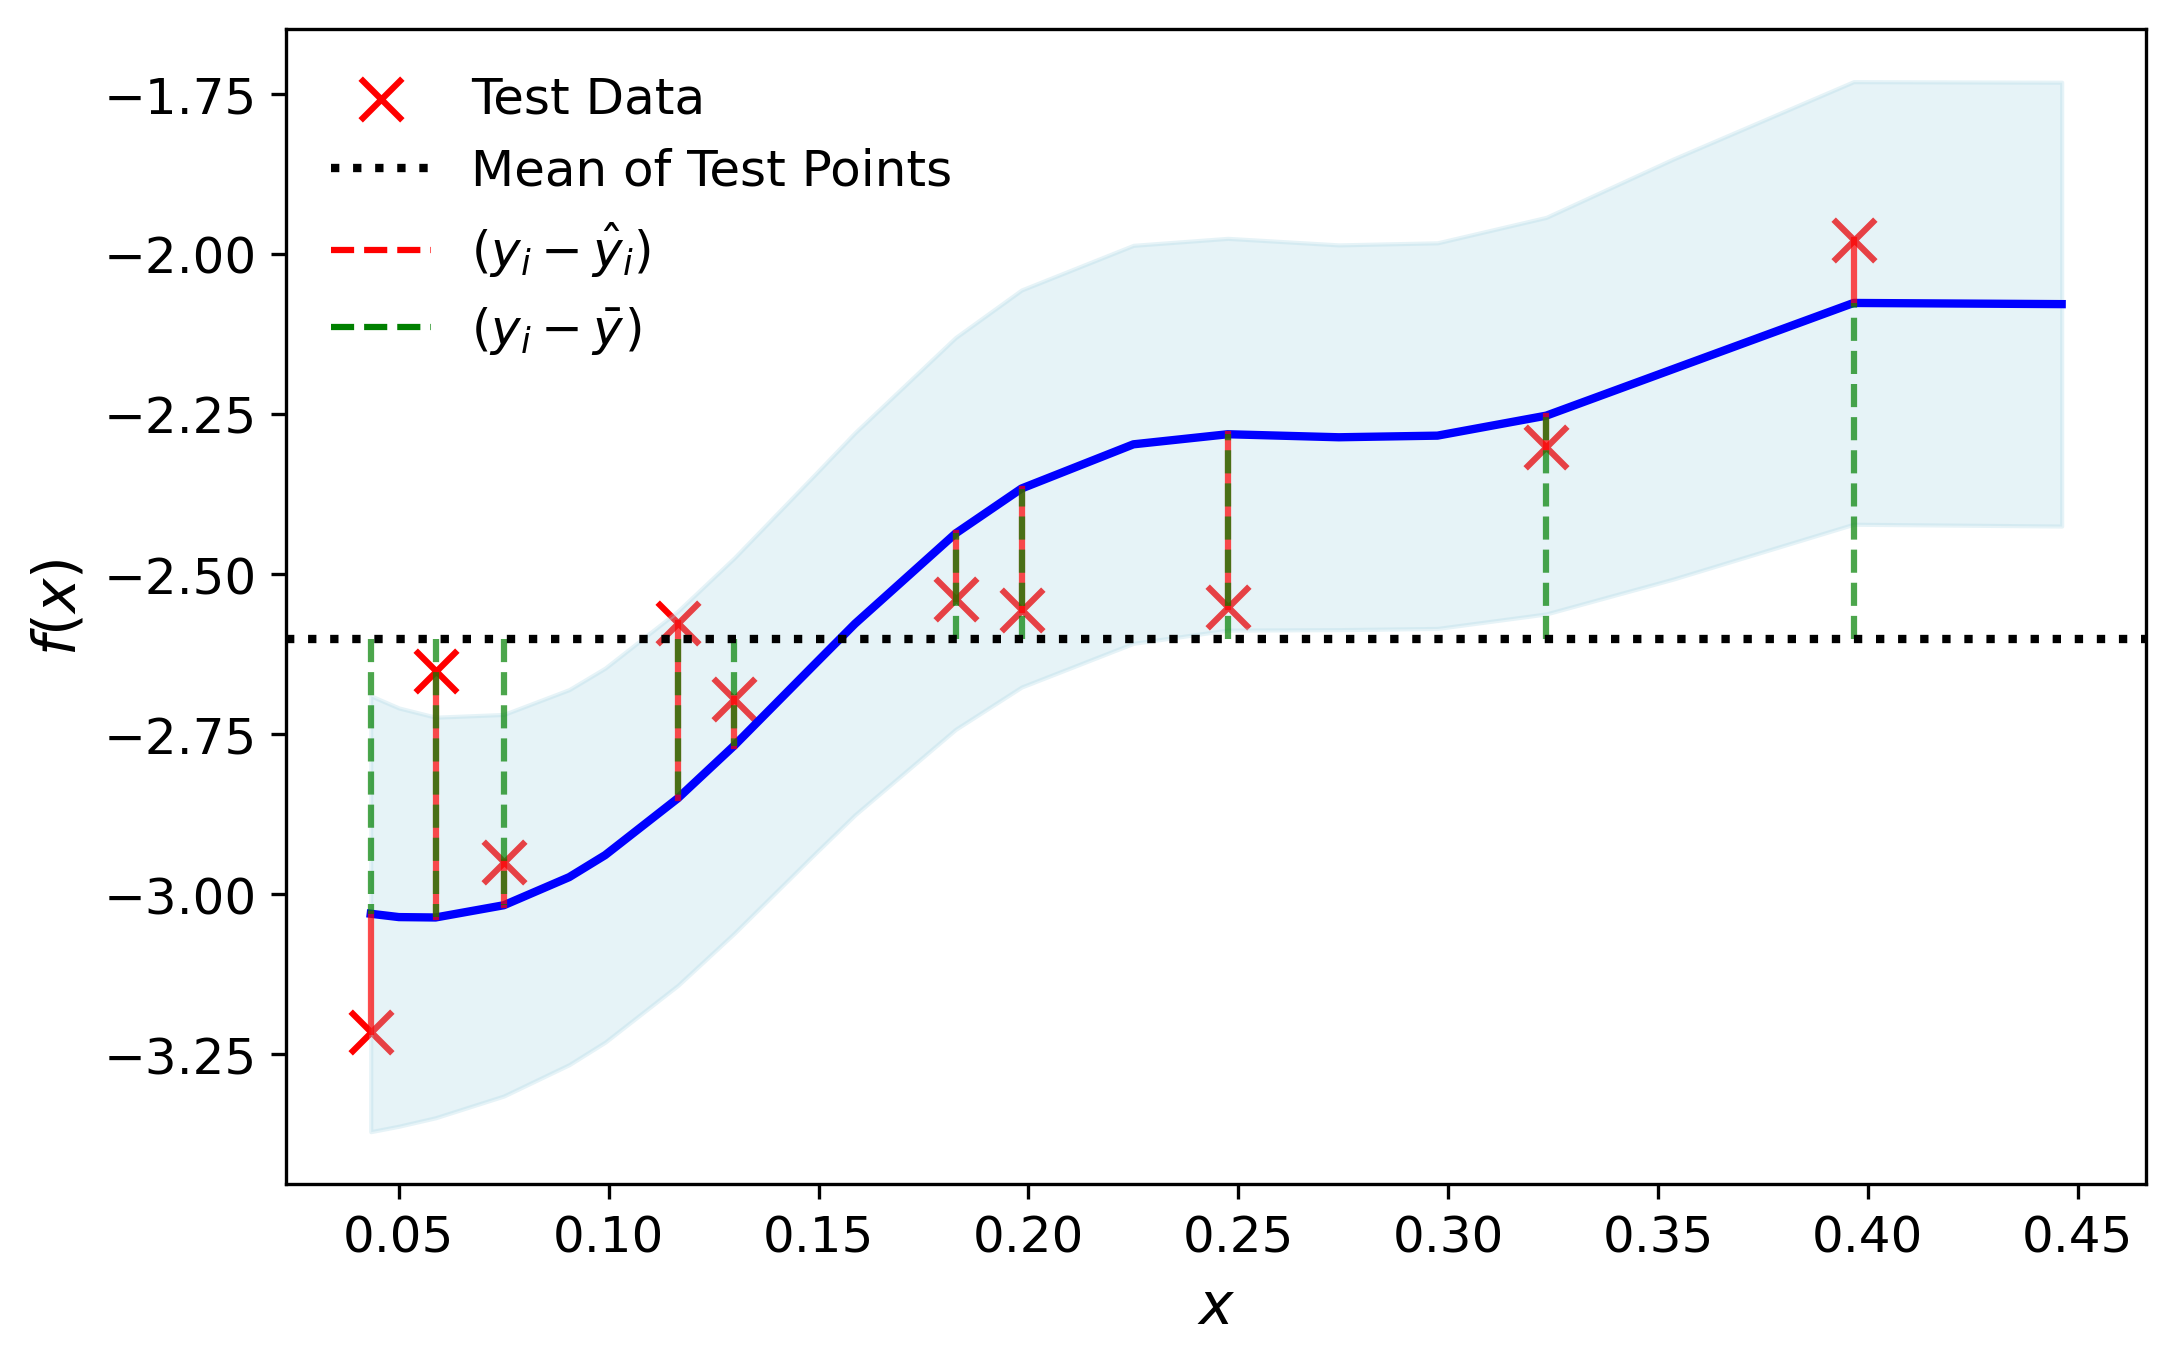
\includegraphics[width=3cm]{LatexPlots/1dplots/r2.png}} &  
        \adjustbox{valign=c}{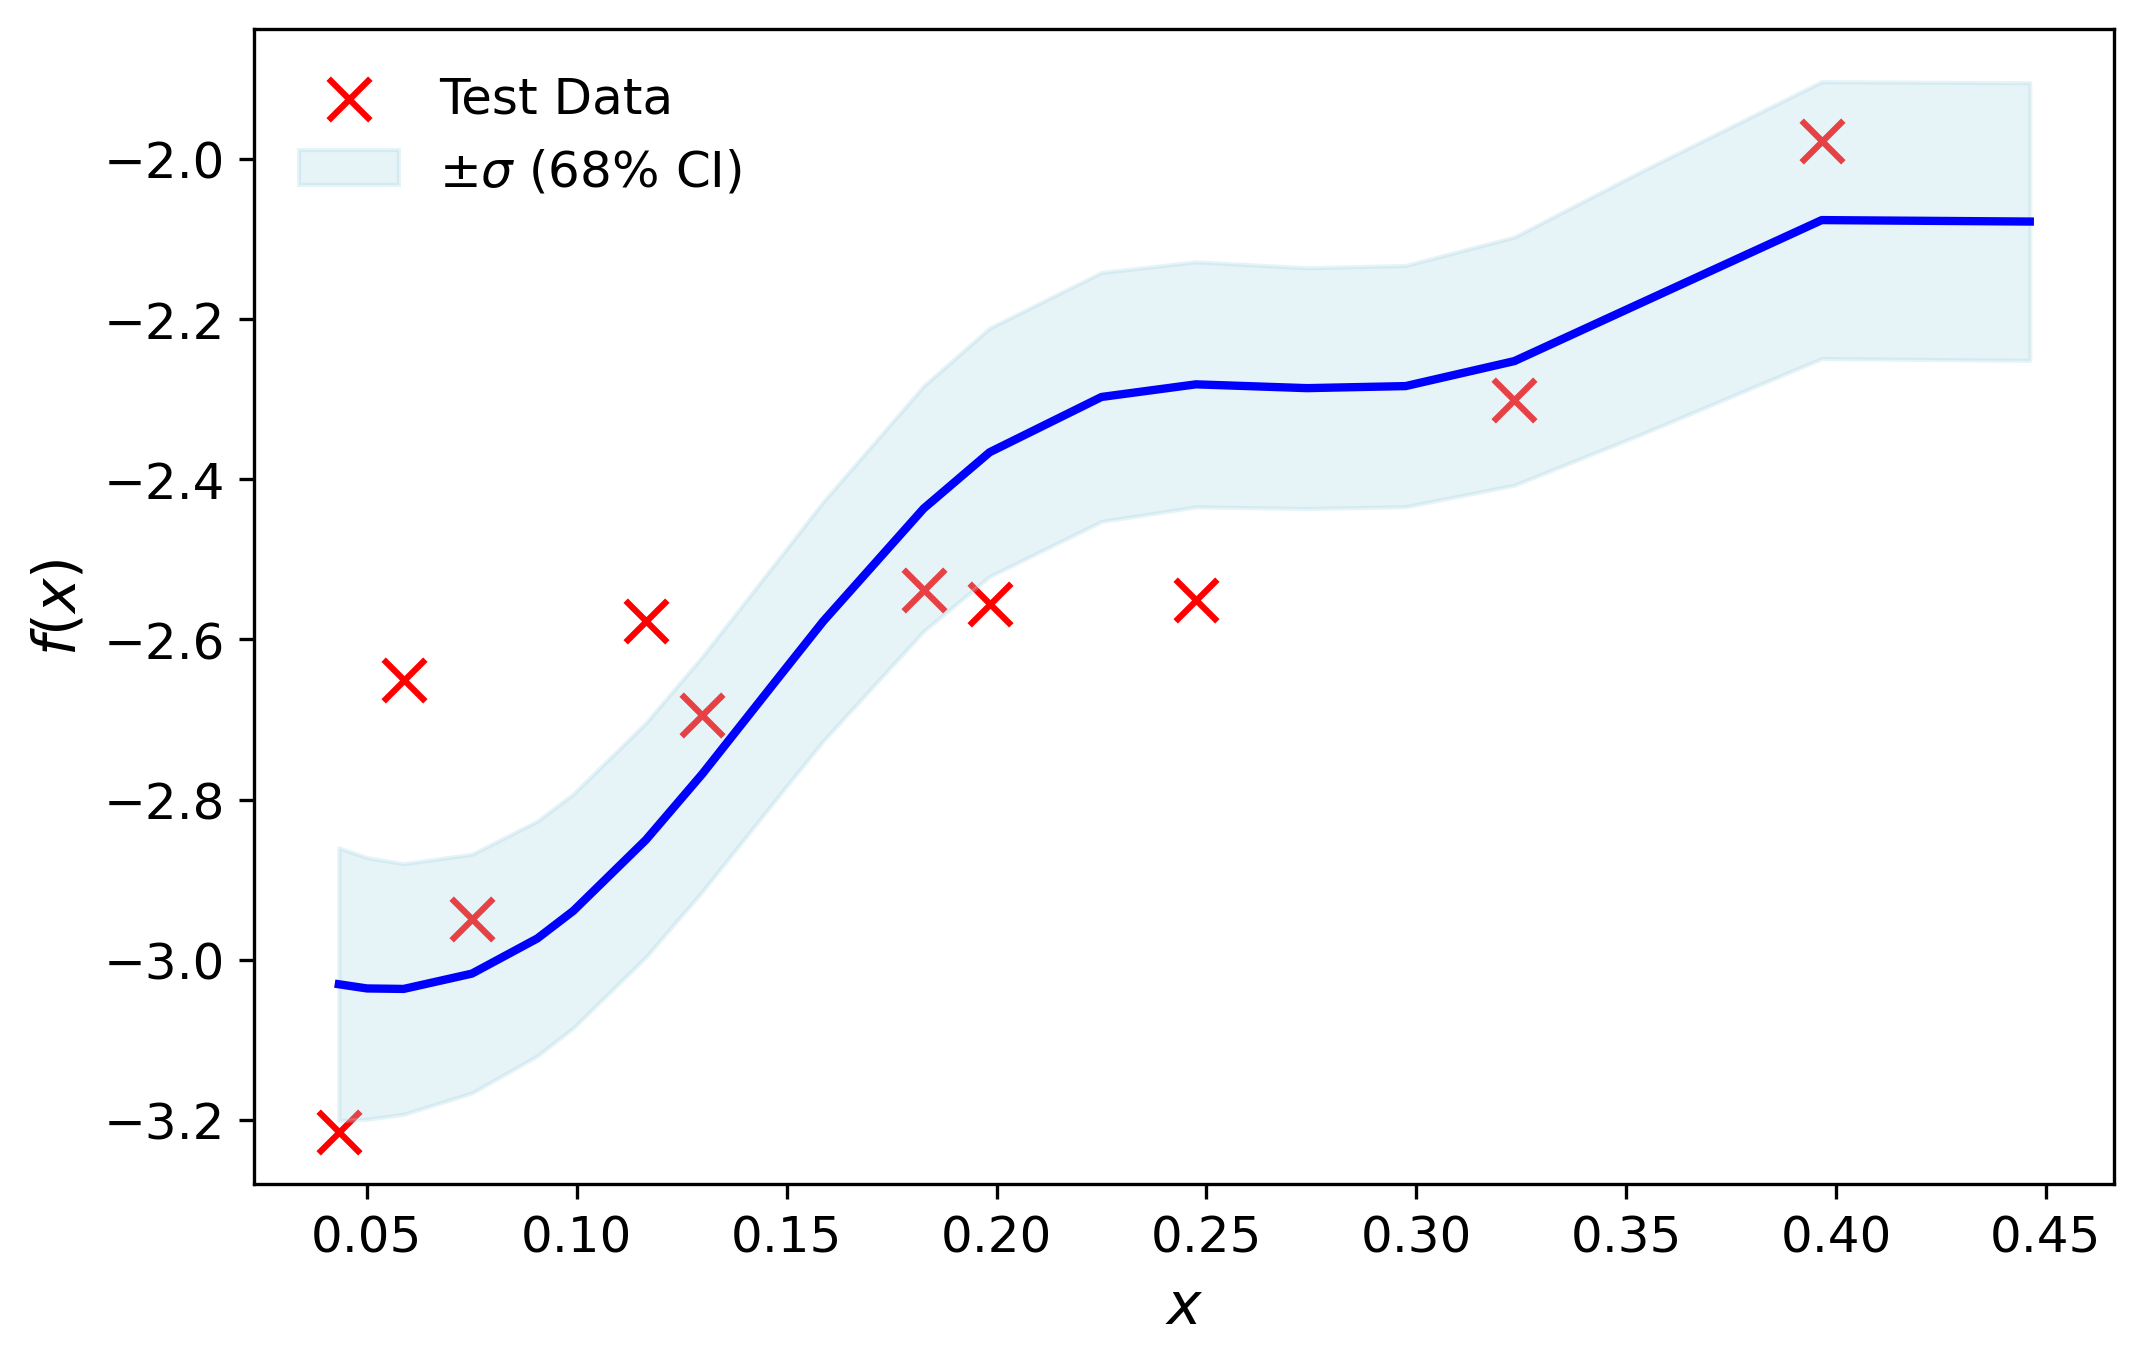
\includegraphics[width=3cm]{LatexPlots/1dplots/fom.png}} &  
        \adjustbox{valign=c}{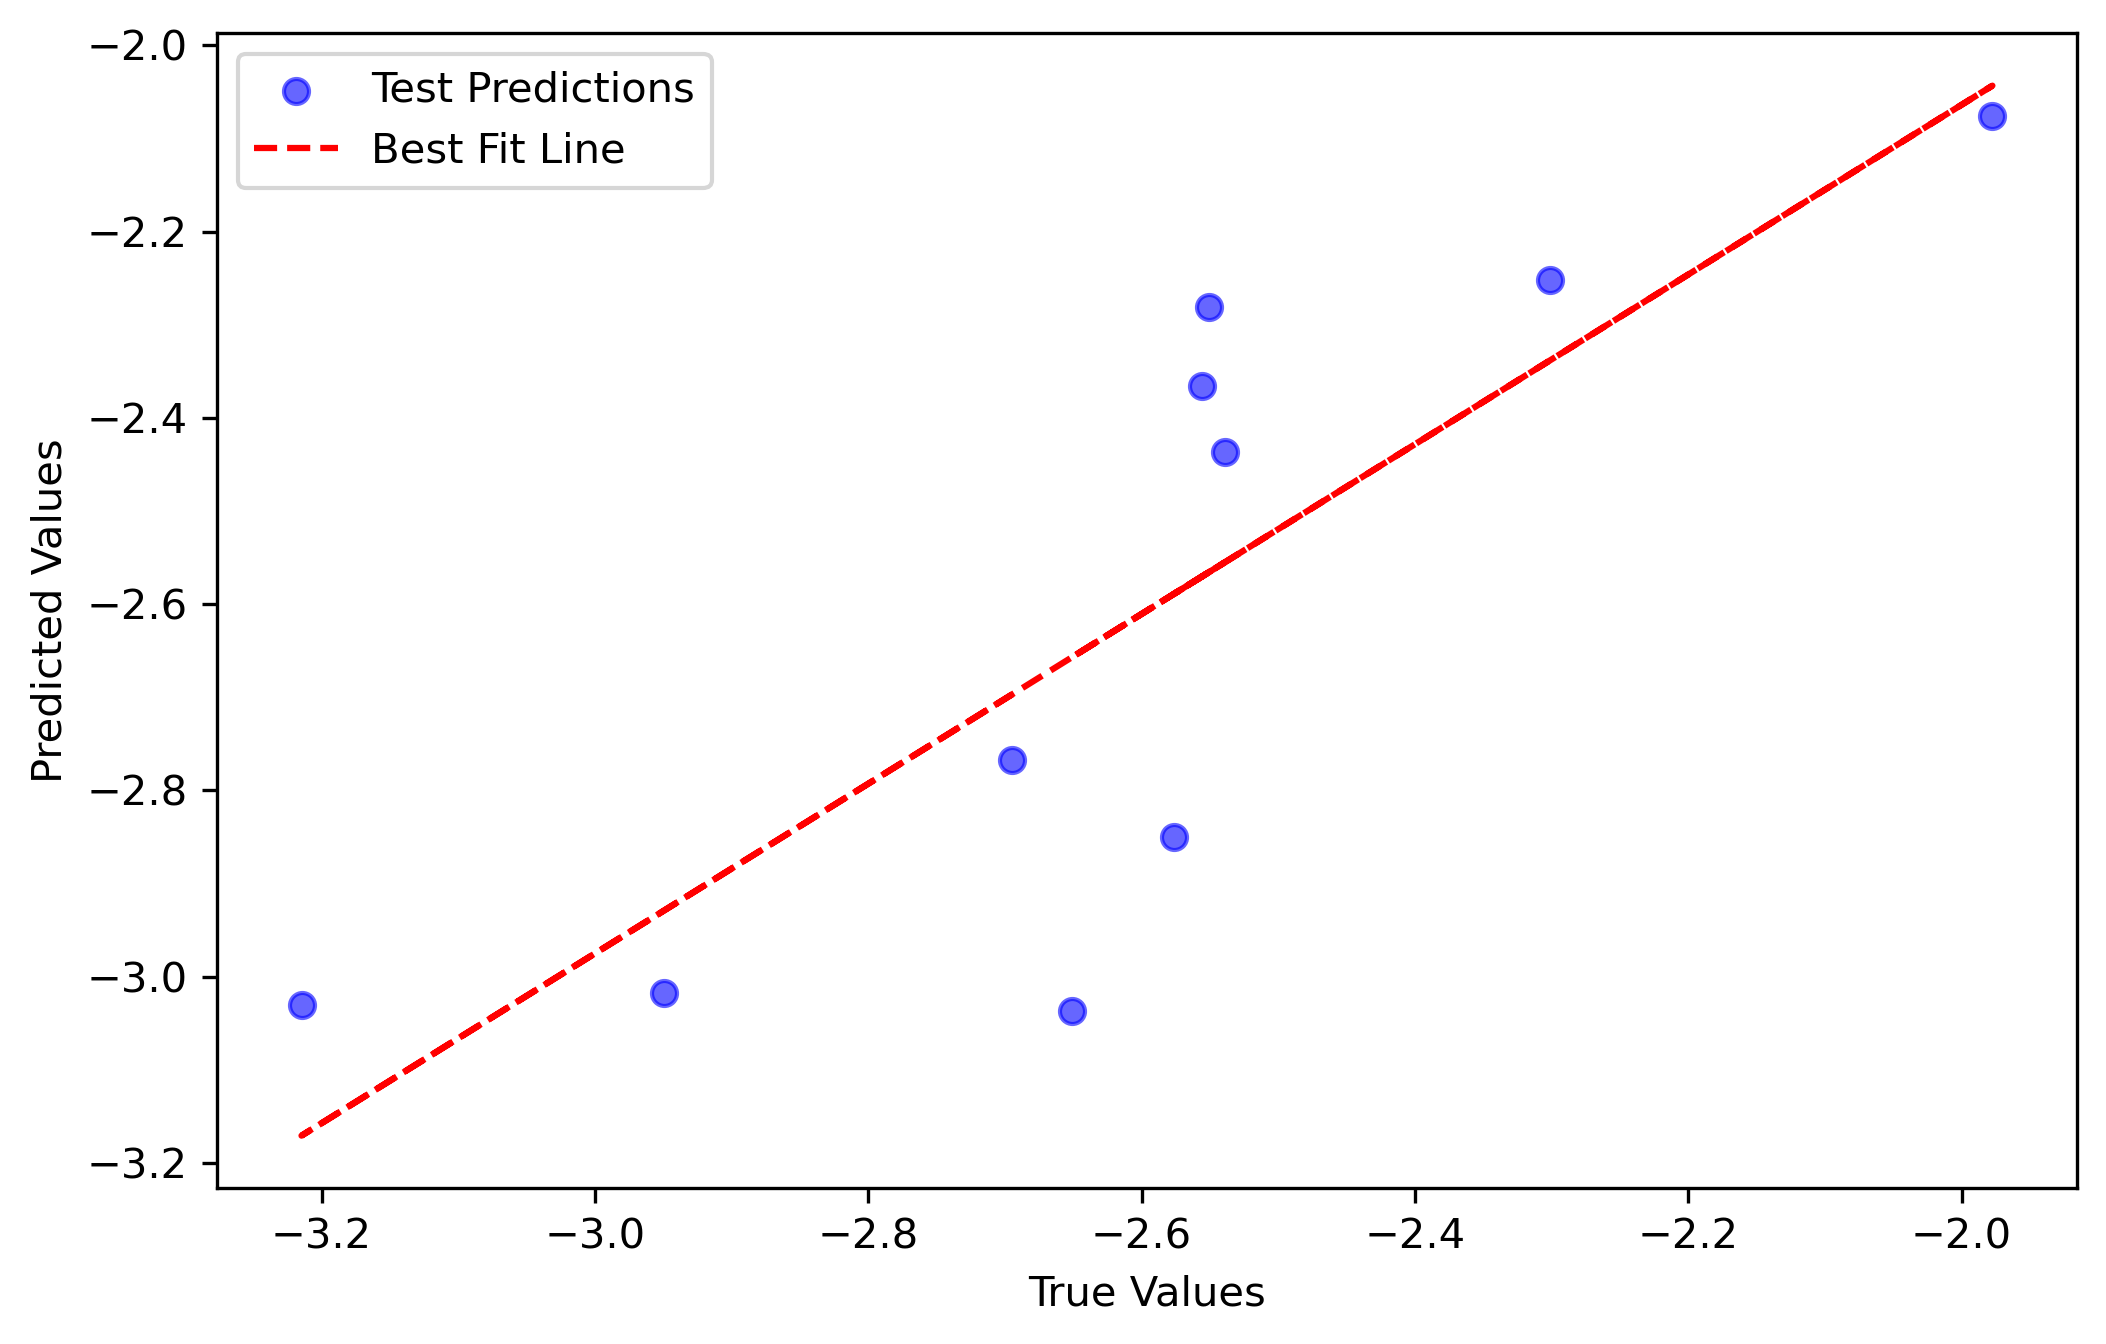
\includegraphics[width=3cm]{LatexPlots/1dplots/pearson.png}} \\  
        \hline
    \end{tabular}
    
    \caption{Comparison of different performance metrics used in evaluating models.  
    RMSE, \( R^2 \), FOM, and the Pearson Coefficient are included.  
    MAE is similar to RMSE but without squaring errors.  
    Adjusted \( R^2 \) accounts for the number of predictors and is slightly modified from \( R^2 \).
    The actual metrics for each graph are: RMSE = 0.2, \( R^2 \) = 0.6, FOM = 1.09, Pearson correlation = 0.8.}
    
    \label{tab:metrics-comparison}
\end{table}

\section{Multi-Dimensional Gaussian Process Regression}

\begin{itemize}
    \item Here we want to bring up how we can have a different length parameter for each dimension of the data.
    \item Get a few plots to demonstrate this maybe.
    \item Important to note noise modelling for all dimensions is the same since just adding to the diagonal of the covariance matrix.
    \item Mention how hyper-parameter optimisatino changes in the larger parameter space
\end{itemize}


\section{Method}

\begin{figure}[H]
    \centering
    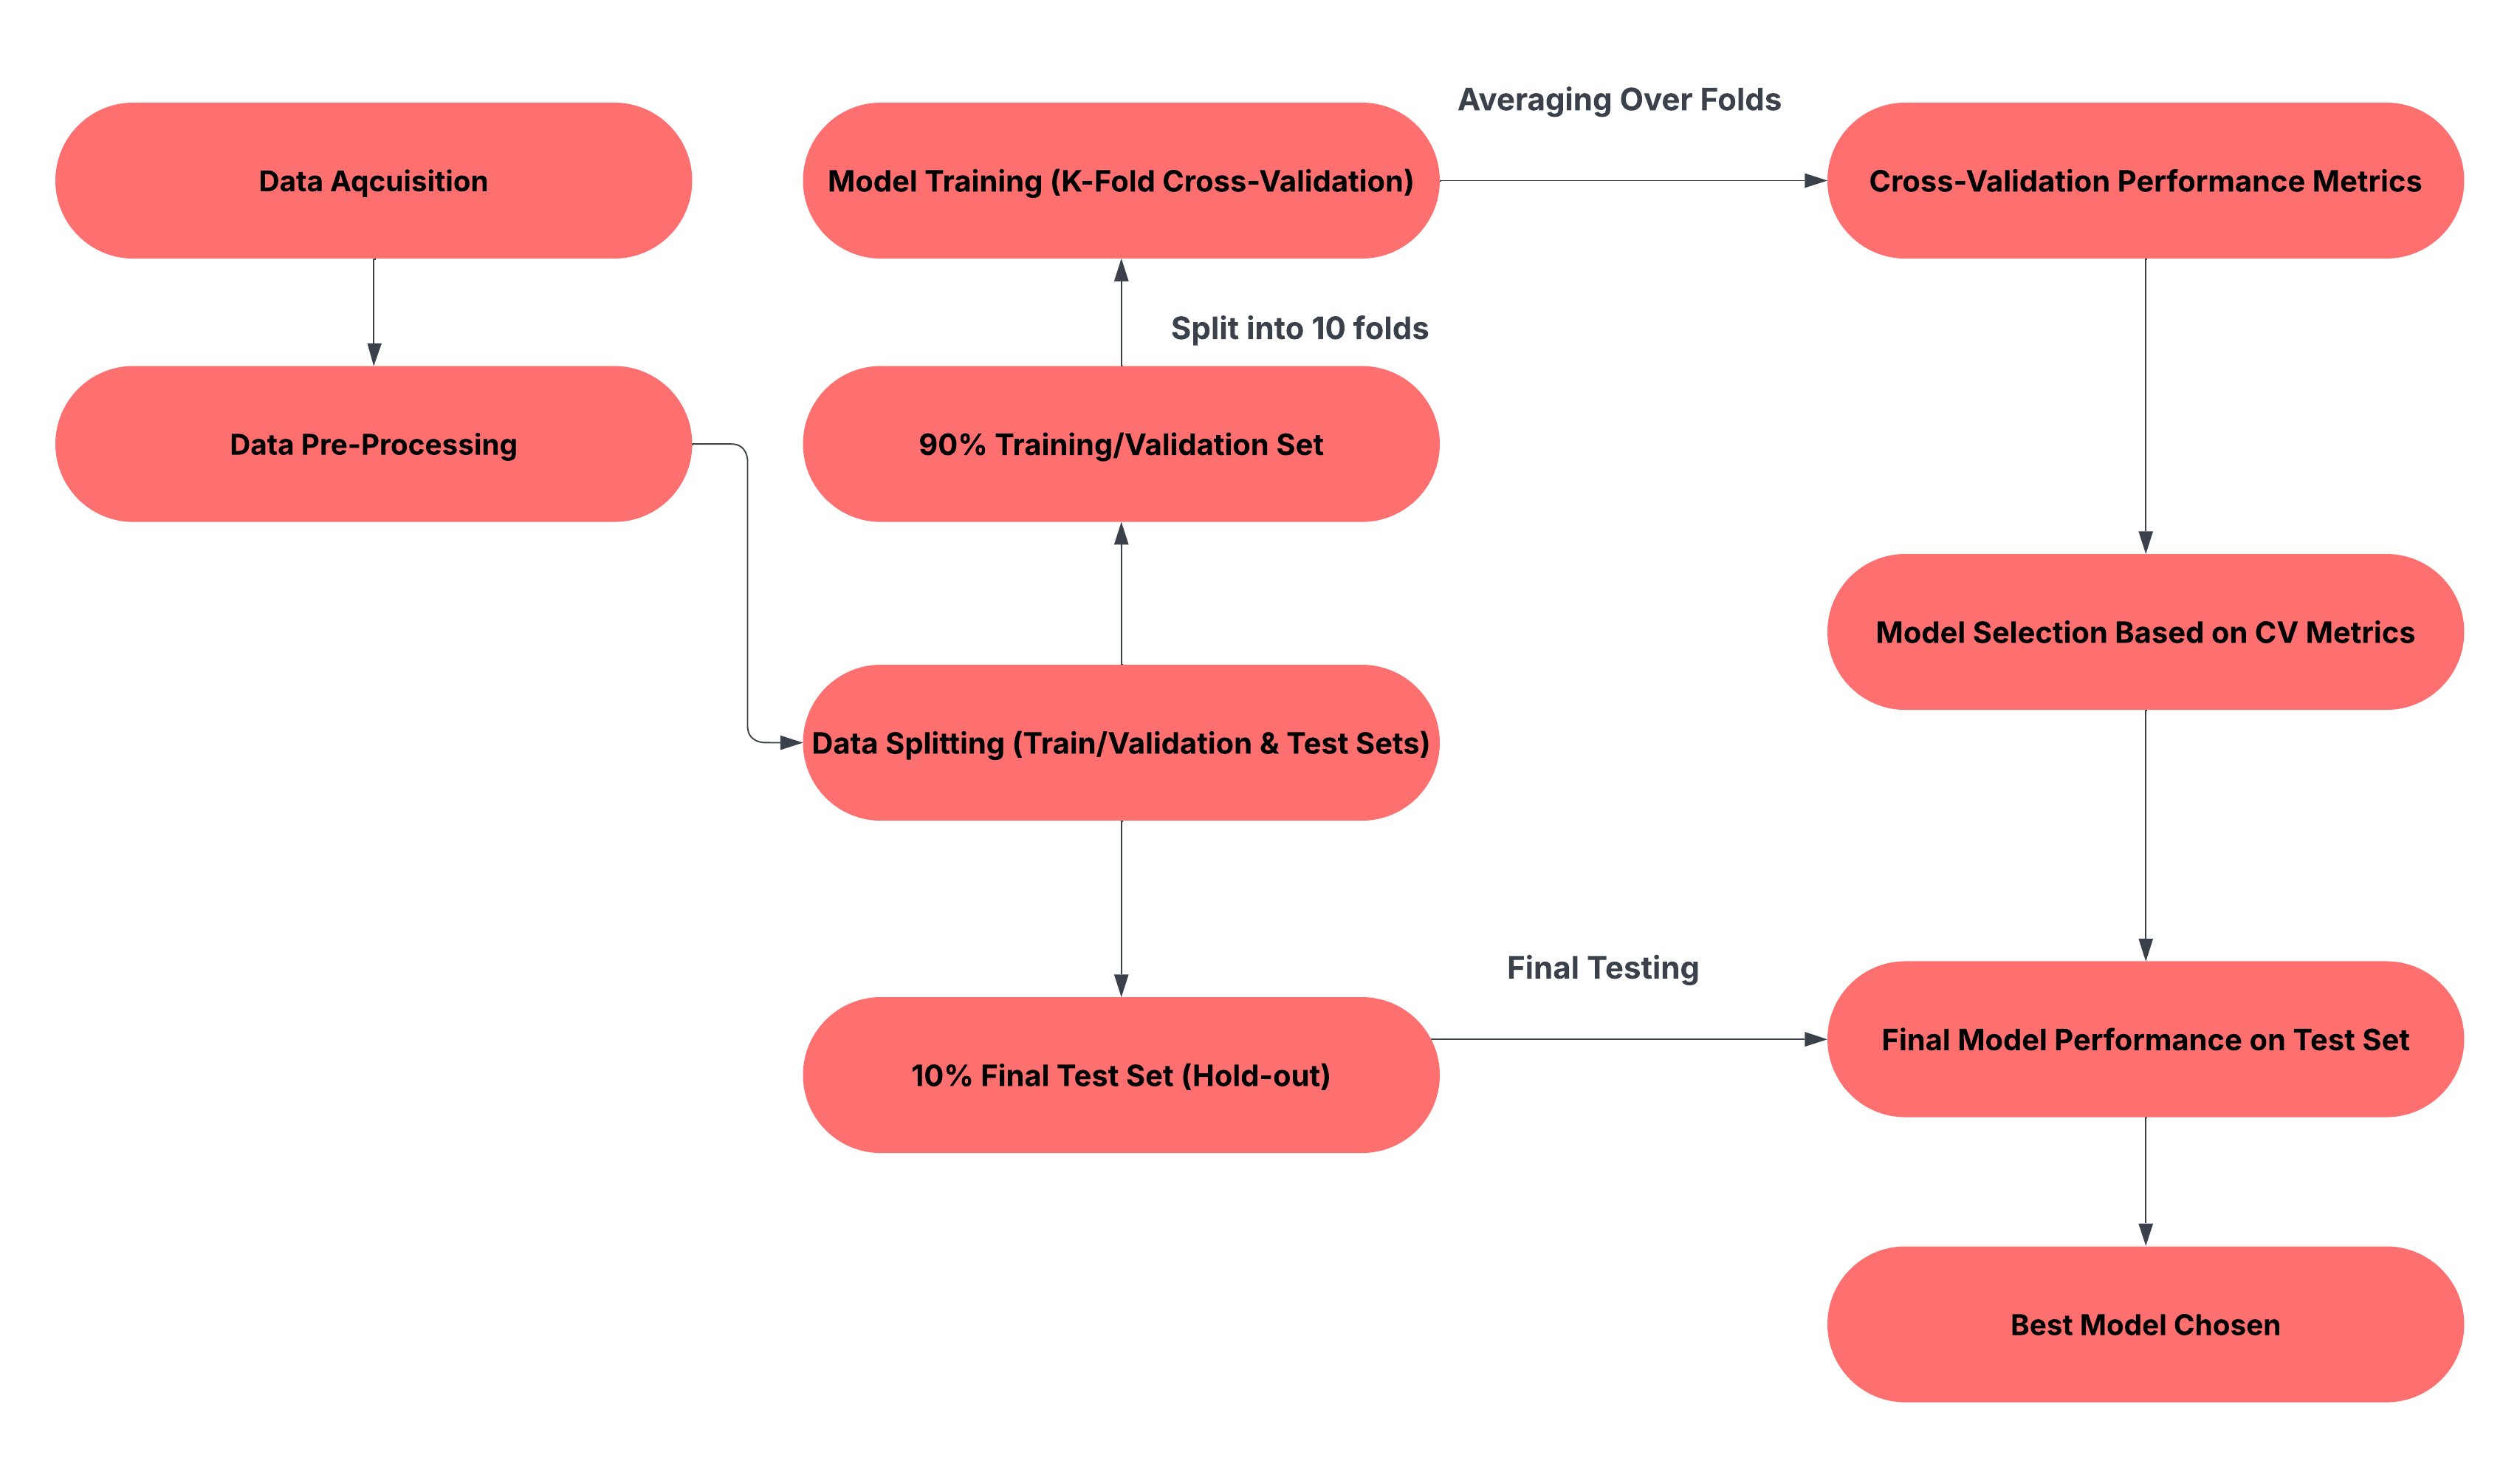
\includegraphics[width=0.8\textwidth]{LatexPlots/Flowchart.png}
    \caption{My Process Flowchart}
    \label{fig:flowchart}
\end{figure}

\subsection{Method Over-view}
Here I will refer back to my 1d examples. The three ways I have to model noise discussed in section \ref{sec: Handlingnoise} are
\begin{itemize}
    \item Using the true error associated with the data.
    \item Using a White Kernel to create a noise hyper parameter which can be optimised
    \item Using Monte Carlo Sampling to sample from the error
\end{itemize}

My different kernels are
\begin{itemize}
    \item RBF
    \item Matern
    \item Laplace
    \item Periodic
    \item Rational Quadratic
\end{itemize}

\subsection{My data 4D - 7D}
\textcolor{red}{Could be discussed in the intro also}
\subsection{Training and Testing Protocol}
As \ref{fig:flowchart} details I divided my data in a 90\% train and validation data set and then a final 10\% data test left untouched for testing.
I split my training and validation data into 10 folds and trained my model on each of these 10 folds. 



\begin{itemize}
    \item Different Models (handling error and optimisation)
    \item split data into 90-10. 90 train and validation and 10 test
    \item Evaluated using cross validation and multiple metrics
    \item compared and found best model
    \item built these final models on the 90\% of the data
    \item tested on the 10\% of the data
    \item Also built MCMC using the gpr methods that made to final
    \item Used this to build a posterior on the hyper-parameters
    \item Compared MCMC solutions to the optimised solutions
\end{itemize}

\section{Different Models}
\begin{itemize}
    \item White Kernel without Error Knowledge
    \item White Kenrel With Error Knowledge
    \item Using $\alpha = err^2$
    \item Using Monte Carlo Sampling, Sampling from the Error
    \item Using MCMCing to build a posterior on hyper-parameter distribution
    \item Picking values from this posterior distribution to use
\end{itemize}


%\printbibliography
\bibliography{references}

\end{document}


